% This is a template for Ph.D. dissertations in the UCI format.
% 
% All fonts, including those for sub- and superscripts, must be 10
% points or larger.  Recommended sizes are 14-point for chapter
% headings, 12-point for the main body of text and figure/table
% titles, and 10-point for footnotes, sub- and super-scripts, and text
% in figures and tables.
%
% Notes: Add short title to figures, sections, via square brackets,
% e.g. \section[short]{long}.
%
\documentclass[12pt,fleqn]{ucithesis}

% A few common packages
\usepackage{amsmath}
\usepackage{amsthm}
\usepackage{amssymb}
\usepackage{array}

\usepackage{graphicx}
\usepackage{url}

\usepackage{natbib}
\usepackage{relsize}

% Some other useful packages
\usepackage{caption}
\usepackage{subcaption}  % \begin{subfigure}...\end{subfigure} within figure
\usepackage{multirow}
\usepackage{tabularx}

\usepackage{listings}

\usepackage{color}  %to leave some notes

\makeatletter
\newif\if@restonecol
\makeatother
\let\algorithm\relax
\let\endalgorithm\relax
\usepackage[linesnumbered]{algorithm2e}

\usepackage[normalem]{ulem}

\makeatletter
\newcommand{\nosemic}{\renewcommand{\@endalgocfline}{\relax}}% Drop semi-colon ;
\newcommand{\dosemic}{\renewcommand{\@endalgocfline}{\algocf@endline}}% Reinstate semi-colon ;
\newcommand{\pushline}{\Indp}% Indent
\newcommand{\popline}{\Indm\dosemic}% Undent
\makeatother

% plainpages=false fixes the "duplicate ignored" error with page counters
% Set pdfborder to 0 0 0 to disable colored borders around PDF hyperlinks
\usepackage[plainpages=false,pdfborder={0 0 0}]{hyperref}

% Uncomment the following two lines to use the algorithm package,
% which provides an algorithm environment similar to figure and table
% ("\begin{algorithm}...\end{algorithm}"). A list of algorithms will
% automatically be added in the preliminary pages. Note that you
% probably want a package for the actual code to go with this (e.g.,
% algorithmic).
%\usepackage{algorithm}
%\renewcommand{\listalgorithmname}{\protect\centering\protect\Large LIST OF ALGORITHMS}

% Uncomment the following line to enable Unicode support. This will allow you
% to enter non-ASCII characters (such as accented characters) directly without
% having to use LaTeX's awkward escape syntax (e.g., \'{e})
% NOTE: You may have to install the ucs.sty package for this to work. See:
% http://www.unruh.de/DniQ/latex/unicode/
%\usepackage[utf8x]{inputenc}


% Modify or extend these at will.
\newtheorem{theorem}{{\sc Theorem}}[chapter]
\newtheorem{definition}{{\sc Definition}}[chapter]
\newtheorem{example}{{\sc Example}}[chapter]

% Uncomment the following to have numbered subsubsections (by default
% numbering goes only to subsections).
%\setcounter{secnumdepth}{4}


% Set this to only select a subset of the includes directives below.
% Very handy to speed up compilation if you're working on a certain
% part of your thesis. It conserves page numbers, references, etc.
% even for non-included files.
%\includeonly{chapter1}

\begin{document}

% Preliminary pages are always loaded (TOC, CV, etc.)
% \thesistitle{
%   Pruning Large Search Spaces using Context Networks
% }

\thesistitle {
  Discovering Real World Context to Tag Personal Photos
}

\degreename{Doctor of Philosophy}

% Use the wording given in the official list of degrees awarded by UCI:
% http://www.rgs.uci.edu/grad/academic/degrees_offered.htm
\degreefield{Computer Science}

% Your name as it appears on official UCI records.
\authorname{Arjun Satish}

% Use the full name of each committee member.
\committeechair{Professor Ramesh Jain}
\othercommitteemembers
{
  Dr. Amarnath Gupta\\
  Professor Nalini Venkatasubramanian\\
  Professor Deva Ramanan\\
  Professor Bill Tomlinson
}

\degreeyear{2013}

\copyrightdeclaration
{
  {\copyright} {\Degreeyear} \Authorname
}

% If you have previously published parts of your manuscript, you must list the
% copyright holders; see Section 3.2 of the UCI Thesis and Dissertation Manual.
% Otherwise, this section may be omitted.
% \prepublishedcopyrightdeclaration
% {
% 	Chapter 4 {\copyright} 2003 Springer-Verlag \\
% 	Portion of Chapter 5 {\copyright} 1999 John Wiley \& Sons, Inc. \\
% 	All other materials {\copyright} {\Degreeyear} \Authorname
% }

% The dedication page is optional.
\dedications
{
  \textit{And it's whispered that soon, if we all call the tune,} \\
  \textit{Then the piper will lead us to reason} \\
  \textit{And a new day will dawn for those who stand long} \\
  \textit{And the forest will echo with laughter} \\ 
  \textit{} \\
  \setlength{\parindent}{6.3cm} \texttt{Jimmy Page \& Robert Plant, } \\
  \setlength{\parindent}{7cm} \texttt{from Stairway to Heaven, 1970} \\
}

\acknowledgments
{

I would like to thank my advisors, Ramesh Jain and Amarnath Gupta for teaching me the values and fundamental principles of the scientific method. Without their continuing support, a project like CueNet would have barely made this far. The many technical and personal discussions I had with them during the last few years are going to be greatly missed. I owe a lot to Ramesh for accepting me as a graduate student, and introducing me to his beloved projects and ideas and letting me play with them as I seemed fit.

Special thanks to my committee members, Deva Ramanan, Nalini Venakatasubramian and Bill Tomlinson to take the time out to provide feedback on my work and suggesting very interesting experiments which helped me gain some major insights into it. My fellow graduate students at ISG were always a source of inspiration and encouragement to work on challenging cross-domain problems. 

My friends at the Experiential Systems Laboratory: Setareh, Hamed, Laleh and Siripen deserve a huge reward for putting up with me these past few years. They have always been extremely supportive and took the time to provide enormous amounts of feedback and ideas to improve all the projects I have worked on. Many thanks to them for helping shape the ideas presented in the following pages.

A special thanks to Alex Thornton, Chen Li and Mike Carey to help me understand the teacher's side of the table at universities. Working with them has helped me understand how I can change the world in small steps by guiding students the right way. Big thanks to the students whom I worked with during the last five years here. 

I owe my best friends Shekhar and Karthik for patiently bearing my tantrums for the last decade. Without Shekhar’s persistent pushes, I would have never applied to graduate school. Big thanks to them for introducing me to the world of music, which colors many of the gray days.

Hearty thanks to Amrish, Ronen and Liat to introducing me to various events during my first days at the USA. They helped me explore various aspects of life in UCI, which I would have never been exposed to otherwise.

A big thanks to my dear friends Alex, Nick, Stephanie, Vinnie, Joel, Ashley, Sameer, Alegria and Reuben for all the barbecues, wine nights, dessert parties, concerts and all the other kinds of activities which made the last few years so memorable. A small apology to Alex and Nick for stopping them halfway each time we decided to run a few miles together.

Sincerest thanks to my family, and friends, Shweta, Sidharth and Natasha for helping me through the ups and downs of life. This dissertation would have been impossible without your help. 

}


% Some custom commands for your list of publications and software.
\newcommand{\mypubentry}[3]{
  \begin{tabular*}{1\textwidth}{@{\extracolsep{\fill}}p{4.5in}r}
    \textbf{#1} & \textbf{#2} \\ 
    \multicolumn{2}{@{\extracolsep{\fill}}p{.95\textwidth}}{#3}\vspace{6pt} \\
  \end{tabular*}
}
\newcommand{\mysoftentry}[3]{
  \begin{tabular*}{1\textwidth}{@{\extracolsep{\fill}}lr}
    \textbf{#1} & \url{#2} \\
    \multicolumn{2}{@{\extracolsep{\fill}}p{.95\textwidth}}
    {\emph{#3}}\vspace{-6pt} \\
  \end{tabular*}
}

% Include, at minimum, a listing of your degrees and educational
% achievements with dates and the school where the degrees were
% earned. This should include the degree currently being
% attained. Other than that it's mostly up to you what to include here
% and how to format it, below is just an example.
\curriculumvitae
{

\textbf{EDUCATION}
  
  \begin{tabular*}{1\textwidth}{@{\extracolsep{\fill}}lr}
    \textbf{Doctor of Philosophy in Computer Science} & \textbf{2013} \\
    \vspace{6pt}
    University of California, Irvine & \emph{Irvine, CA} \\
    \textbf{MS in Computer Science} & \textbf{2011} \\
    \vspace{6pt}
    University of California, Irvine & \emph{Irvine, CA} \\
    \textbf{BE in Electronics and Communications} & \textbf{2002-2006} \\
    \vspace{6pt}
    Sir MV Institute of Technology & \emph{Bangalore, Karnataka, India} \\
  \end{tabular*}

\vspace{12pt}
\textbf{RESEARCH EXPERIENCE}

  \begin{tabular*}{1\textwidth}{@{\extracolsep{\fill}}lr}
    \textbf{Graduate Research Assistant} & \textbf{2007--2013} \\
    \vspace{6pt}
    University of California, Irvine & \emph{Irvine, California} \\
    \textbf{Research Intern} & \textbf{2010} \\
    \vspace{6pt}
    Microsoft Research & \emph{Mountain View, California} \\
  \end{tabular*}

\vspace{12pt}
\textbf{TEACHING EXPERIENCE}

  \begin{tabular*}{1\textwidth}{@{\extracolsep{\fill}}lr}
    \textbf{Teaching Assistant} & \textbf{2007--2013} \\
    \vspace{6pt}
    University of California, Irvine & \emph{Irvine, California} \\
  \end{tabular*}

\vspace{12pt}
\textbf{SELECTED HONORS AND AWARDS}

  \begin{tabular*}{1\textwidth}{@{\extracolsep{\fill}}lr}
    \textbf{Google, Ph.D. Fellowship} & \textbf{2012} \\
    \vspace{6pt}
    Google, Inc.\\

    \textbf{Hitec Octane Entrepreneurship Competition} & \textbf{2008} \\
    \vspace{6pt}
    Second Prize & \emph{Irvine, California} \\
  \end{tabular*}

\pagebreak

\textbf{REFEREED CONFERENCE PUBLICATIONS}

  \mypubentry{CueNet: a Context Discovery Framework to Tag Personal Photos}{Mar 2013}{ICMR 2013}  
  \mypubentry{Visualizing Progressive Discovery}{Mar 2013}{ICMR 2013}  
  \mypubentry{Tolkien: An Event Based Storytelling System}{Aug 2009}{VLDB 2009}
  \mypubentry{A New Approach for Adding Browser Functionality}{Jun 2008}{Hypertext 2008}

\vspace{12pt}
\textbf{TECHNICAL REPORTS}

  \mypubentry{Context Networks for Annotating Personal Media}{May 2013}{ESL.UCI.EDU-TR 2013-May/01}
  \mypubentry{Tagging Personal Photos Using Contextual Information}{Aug 2012}{Whitepaper}
  \mypubentry{Lives: A System for Creating Families of Multimedia Stories}{Aug 2010}{MSR-TR-2011-65}
  \mypubentry{Tolkien: Weaving Stories from Personal Media}{Jun 2010}{ESL.UCI.EDU-TR 2010/04/11}

\vspace{12pt}
\textbf{SOFTWARE}

  \mysoftentry{CueNet}{https://github.com/wicknicks/cuenet/}
  {Polyglot implementation of the CueNet ecosystem to tag faces in photos.}

}

% The abstract should not be over 350 words, although that's
% somewhat of a soft constraint.
\thesisabstract
{
Automatic annotation algorithms assign one or more labels from a candidate search space to a given input object. The collection of these labels is either constructed manually, or derived from a set of sources. It is known that the accuracy of annotation algorithms is typically a decreasing function of the number of labels in the search space. In annotating real-world multimedia objects, this search space quickly explodes if not carefully curated. In this work, we present a technique to prune search spaces yet retain a very large number of correct tags for a multimedia object. Specifically, we shall address pruning of search spaces for the problem of tagging faces in the photo media.

Photos capture the momentary state of real-world entities. Any knowledge of the state of entities in the real world at the time of photos capture provides useful context to eliminate candidates in the search space. For example, people in Japan cannot appear in photos taken at Paris, and photos taken at an academic conference will largely contain people who work in the same field. 

In the real world, relations between entities change rapidly. It is not possible to use a static model of entity relationships to reason over faces in photo instances taken across a wide range of time. Thus, it is imperative that any system first \textit{discover} the set of relationships which are true at the time of photo capture before pruning the search space.

In this dissertation, we adopt a \textbf{relation-centric view} of real-world contextual information to design and implement a framework, \textbf{CueNet} to discover real-world context. The primary contribution of this dissertation is a \textbf{progressive discovery algorithm} to identify relationships between real-world events and objects. CueNet uses these relationships to reason which objects could appear in a given photos, and uses image features to confirm its hypotheses. People often co-occur across photos. We present a method to \textbf{propagate} objects from neighboring photos to a new untagged photo. We shall extend the concepts behind the PageRank algorithm, used to rank web pages, to order real-world objects, and design score propagation techniques based on event semantics. We present \textbf{experiments} on both real-world photos and simulated events. We implement a system using CueNet to tag thousands of personal photos captured by multiple users, to study the efficacy of using context discovery in pruning search spaces. We also present simulation experiments to measure the time and space complexity of large scale discovery operations. We present the convergence characteristics and results on our real-world datasets to show the utility of the propagation algorithm. 

Finally, we conclude the dissertation by presenting challenging problems for future research and ideas for new applications which can be designed using the foundations of context discovery techniques.
}


%%% Local Variables: ***
%%% mode: latex ***
%%% TeX-master: "thesis.tex" ***
%%% End: ***

\preliminarypages

% Include the different components of your thesis, in separate files.
% Using \include allows you to set \includeonly above.
\chapter{Introduction}

This dissertation introduces a new approach to discovering context for photo annotation problems. The primary complexity of photo annotation problems lie in their large search spacesand the diversity of feature-based representations of images. Contextual information is used to prune this large search spaces with reduced dependency on image features. Once the search space has been reduced, the image features are used to select from the \textit{remaining} tags. For example, people with weak social ties do not co-occur often in photos, and by identifying one we can eliminate the other. In this case, we would say that social context is used to prune candidates in a face annotation problem.

Recently, there have been two changes in the scientific community which motivates us to take a fresh look at context. First, with mobile phones becoming the primary mode of photo taking, the nature of context has evolved from providing cues about tags, to the description of the world around a photo taking moment when a person was taking the photo. With the ever increasing amount of personal, social and public information, it is becoming harder to specify which subset of these would constitute the most interesting context for a given picture. Thus, it is not clear what data to consider context, and how do we combine them to form models of the real world which will allow photo annotation algorithms to reason what tags to assign various regions in a given photo.

More specifically, we address the problem of constructing computational representations of real world events from various heterogeneous data sources, to reason which parts of the search space can be pruned without hurting the overall performance of the annotation algorithm. We refer to such a representation as the \textbf{Context Network} of the photo. The network describes real-world events occurring in the environment, the entities participating in them, and their semantic inter-relationships.

\begin{figure}[t]
\centering
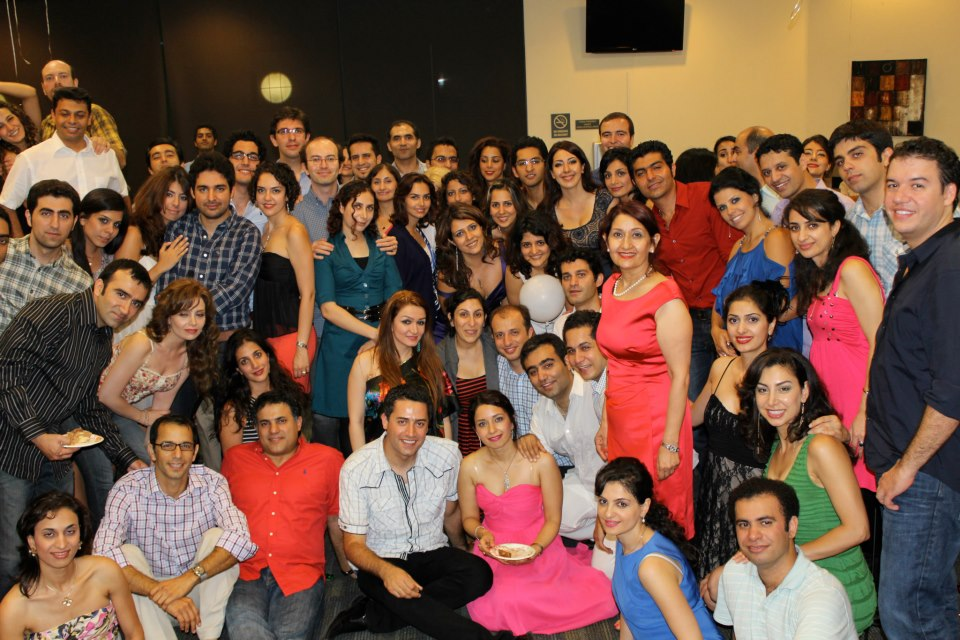
\includegraphics[width=0.8\textwidth]{media/chapter1/setarehetal}
\caption{Face tagging problems could be challenged by very large search spaces.}
\label{fig:people}
\end{figure}

\section{Importance of Context Discovery}

Computer science is moving towards solving real world problems. Social network analysis, medical diagnosis prediction, philanthropic engineering, monitoring public interests through real time communication networks, and situation-based advertising are some of the emerging applications in our area. The common requirement for all of them is to construct models of the real world events occurring in the world, who is participating in them and their attributes and relationships. A technology to construct such a model from various data sources currently available today can play a key role in the effective functioning of such systems.

For the purposes of this dissertation, we propose context discovery techniques in the light of photo annotation problems alone, but the technology and ideas are not tightly coupled with any singly media, and can be easily migrated to assist in solving any problem which requires models of real world events.

\section{Novelty}

Context has been used to address many multimedia problems \cite{henter2012tag, li2012fusing, naaman2005identity, o2009context,stone2008autotagging}. For example, time and location information or social network information from Facebook to solve the face recognition problem. We refer to such a direct dependency between the search space and a data source as \textbf{static linking}. Although these systems are meritorious in their own right, they suffer from the following drawbacks: they are tightly coupled with a few data sources, the unavailability of which would reduce the efficiency of the system, do not employ multiple sources, and therefore the \textbf{relations} between them. 

\begin{figure}[t]
\centering
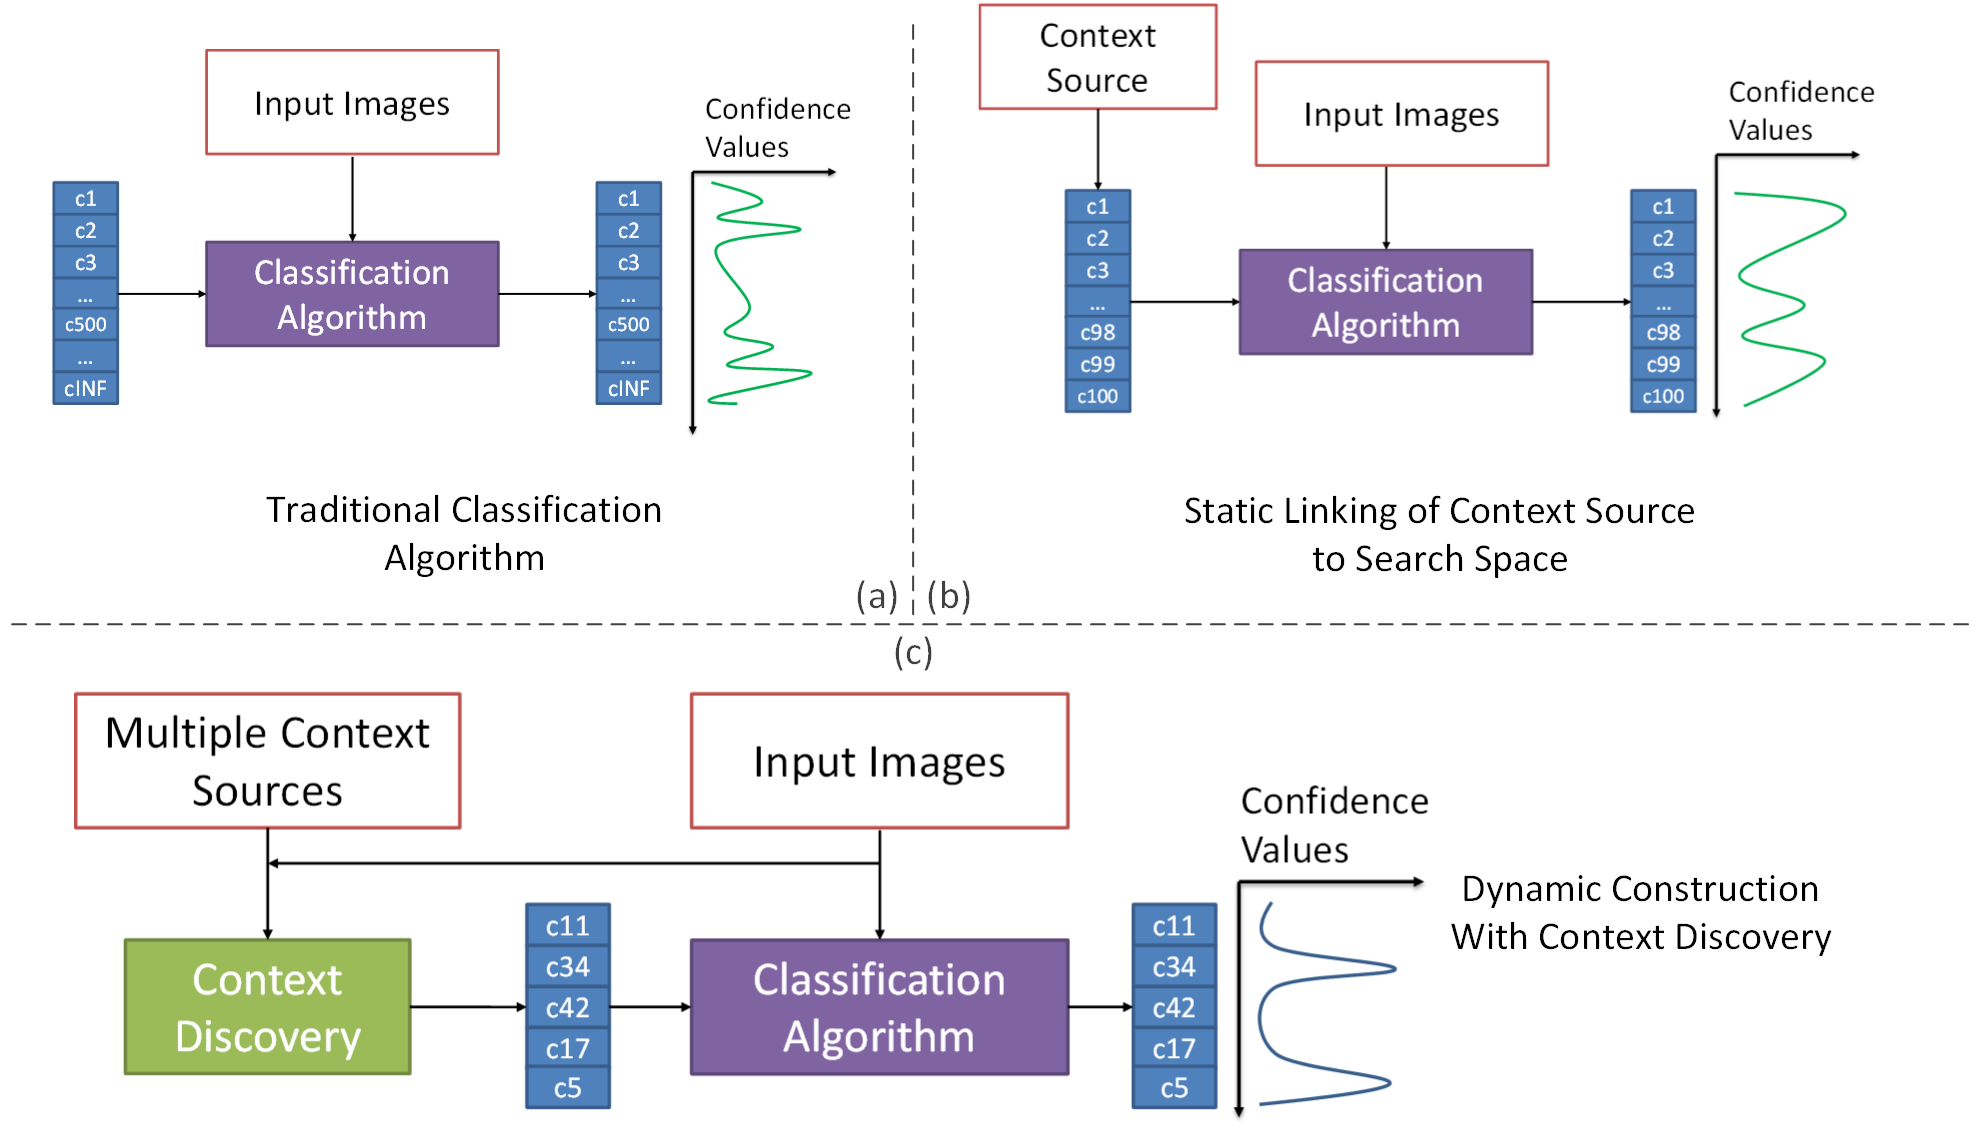
\includegraphics[width=0.85\textwidth]{media/with-without-cuenet-2.png}
\caption{The different approaches in search space construction for a multimedia annotation problem.}
\label{fig:with-without-cuenet}
\end{figure}

Figure \ref{fig:with-without-cuenet} shows the three major ways to prune search spaces in annotation systems. Figure \ref{fig:with-without-cuenet}(a) is one of the earliest system setups where the search spaces were manually constructed, and the focus was mainly on constructing smarter features to correctly classify feature sets \cite{turk1991eigenfaces, belhumeur1997eigenfaces}. Systems like \cite{stone2008autotagging} use a single source like Facebook to populate their search space based on some attributes of the input problem (in this case, the identity of the user). This restricted the search space but it is assumes that all relevant tags will be supplied from the context source, which is usually not correct.

This primary \uline{contribution} of this dissertation is a \textbf{\textit{progressive discovery}} algorithm to ingest information from various real world data sources to construct context networks containing the most relevant information for pruning the search space for the system. Examples of data sources include social media web services to provide information about events and entities like Facebook, Twitter; services which can be queried to find information about places like Yelp; Sensors on personal mobile phones, for example GPS which inform applications of the location of a person is present at any given point in time.

\section{Approach}

\textbf{What is progressive discovery?} Progressive discovery is an incremental process where knowledge of real world events and entities can be added to a given context network. Given a context network and multiple data sources describing events and entities, a progressive discovery algorithm will obtain new information from the sources and relate it to context network. By iteratively executing this algorithm, we can grow a context network until the data sources can provide no further information or the information in the network prunes the search space well enough for the AI problem to be fully solved.

The discussion in the following chapters on context networks and their discovery from various data sources will be presented in conjunction with an application to \textbf{tag faces in personal photos}. The face tagging algorithm, whose search space contains a few million entities attempts to solve a very hard problem. But if a real world model of the world existed, the search space which is relevant to this photo contains just the entities who are present within the field of view of the camera at the time the photo was captured. 

\section{Examples}
Here are two examples of dynamic linking. Figure \ref{fig:example-icmr-hidden} shows a photo of a person about to starting his presentation. Dynamic linking is done in three steps. First, the discovery algorithm proceeds to find the EXIF parameters of the photo, and associates the user with the photo. We call such an event where a photo is associated with its spatio-temporal attributes, a \texttt{photo-capture-event}. It signifies an event where the user is capturing an image with his camera. Second, these attributes are used to discover \textit{what is other events is the owner part of at this time}? Only those data sources are queried which can provide answers to this, and we obtain a response from a conference database saying that the owner was attending the ICMR conference at Dallas, Texas. Third, given this new conference event, the algorithm discovers what were the conference subevents (like keynotes, talks or break sessions) were occurring at this time. Finally, it finds that Mor Naaman and John Smith were speaker and host for the keynote talk going on that time. Given the two candidates, the face tagging algorithm proceeds to identify the correct tag, figure \ref{fig:example-icmr-show}.


\begin{figure}[ht]
\begin{minipage}[b]{0.45\linewidth}
\centering
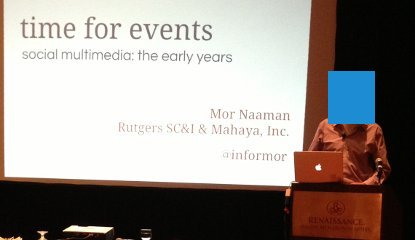
\includegraphics[width=\textwidth]{media/chapter1/icmr-keynote-2-hidden.jpg}
\caption{Who is in this photo?}
\label{fig:example-icmr-hidden}
\end{minipage}
\hspace{0.5cm}
\begin{minipage}[b]{0.45\linewidth}
\centering
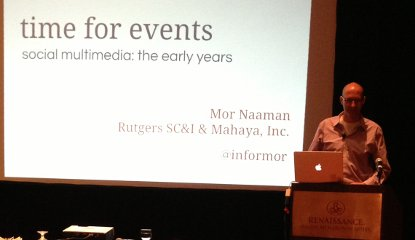
\includegraphics[width=\textwidth]{media/chapter1/icmr-keynote-2-show.jpg}
\caption{Mor Naaman at ICMR.}
\label{fig:example-icmr-show}
\end{minipage}
\end{figure}

Now, lets look at in photo in figure \ref{fig:example-kasturi-hidden}. Context discovery initiates the same way as in the above example, but after searching for events related to the owner in data sources, finds nothing. It proceeds to rank all known contacts according to location, and given that this photo was taken to the owner's workplace ranks colleagues higher than friends. The top 20 (an arbitrary constant) ranked candidates are passed to the face tagging algorithm which finds Ramesh Jain in the photo. But not the person to his right in the photo. But now, the \texttt{photo-capture-event} has an additional participant, Ramesh, whose calendar can be queried to find events in which he was participating. The calendar returns the entry ``Kasturi". The algorithm uses this term to find all Ramesh's contacts to find all people with first or last name ``Kasturi'', and finds his long time friend and colleague ``Rangachar Kasturi''. The face tagging algorithm is invoked with one candidate.

\begin{figure}[ht]
\begin{minipage}[b]{0.45\linewidth}
\centering
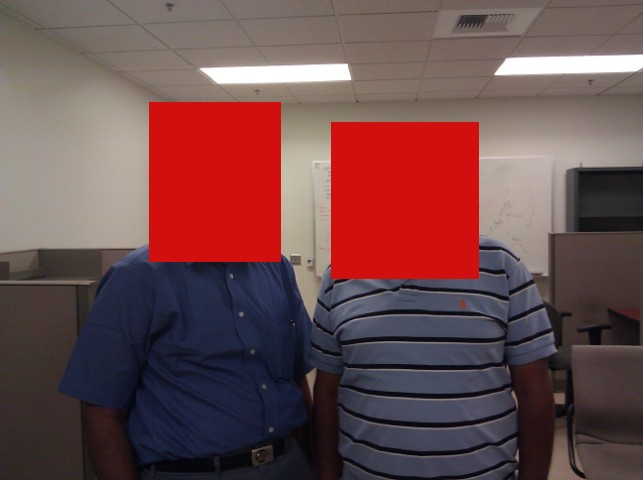
\includegraphics[width=\textwidth]{media/chapter1/kasturi-hidden.jpg}
\caption{Who is in this photo?}
\label{fig:example-kasturi-hidden}
\end{minipage}
\hspace{0.5cm}
\begin{minipage}[b]{0.45\linewidth}
\centering
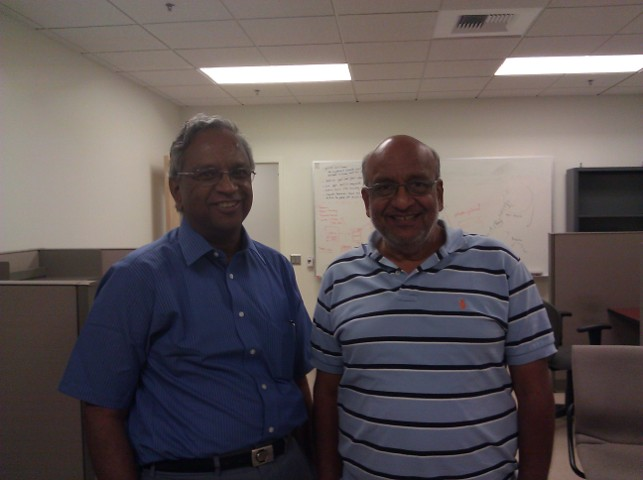
\includegraphics[width=\textwidth]{media/chapter1/kasturi-show.jpg}
\caption{Kasturi and Jain.}
\label{fig:example-kasturi-show}
\end{minipage}
\end{figure}

In this first run, the algorithm linked only to a conference database, whereas in the second case, it used spatial information, personal calendar and contact information. In the later chapters, we will present techniques to represent and link context in a systematic manner.

\section{Overview}
This dissertation is organized into the following chapters. Chapter 2 provides an overview of context, how context has been used to address problems in various scientific disciplines and how we use context in our specific personal photo tagging application. Chapter 3 describes the related work in computer science, and how this work is informed by them. Chapter 4 describes our context discovery framework, how it models various data sources, and how our progressive discovery algorithm constructs models for real world problems. We facilitate this discussion with an example real world application to tag faces of people in personal photos. Chapter 5 analyzes the algorithmic complexity of different parts of the system, and provides experiments to verify the competence and performance of the system. We also present experiments to confirm the efficacy of our approach in the light of the real world application. Finally, chapter 6 attempts to describe the future possibilities of using context discovery in computer science.

% Chapters 6 and 7 describe two extensions to the CueNet framework to solve problems of missing context and that of source selection. 

%% \section{Terminology}
%% Before starting the discussion on Context Networks, it is necessary to include a short note on terminology to avoid any ambiguities. We use the word `Object' to collectively refer to events and entities. An entity includes persons, places in the world, for example `Starbucks, UC Irvine', `The Eiffel Tower, Paris, France', or organizations, for example `Google Inc', `Royal Society of London'. The term `object' has been used in literature to refer to things which have no temporal properties. But, in our discussion, an `object' could imply an event which exhibits temporal properties.

% \begin{figure}[h]
% \centering
% 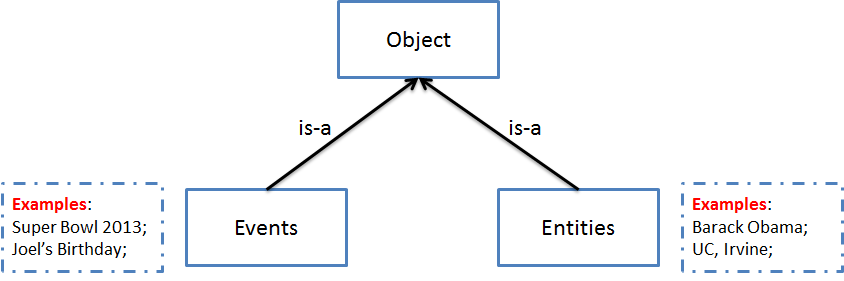
\includegraphics[width=0.75\textwidth]{media/chapter1/terminology.png}
% \caption{Objects, Events and Entities.}
% \label{fig:terminology}
% \end{figure}


% \begin{figure}[ht]
% \begin{minipage}[b]{0.45\linewidth}
% \centering
% 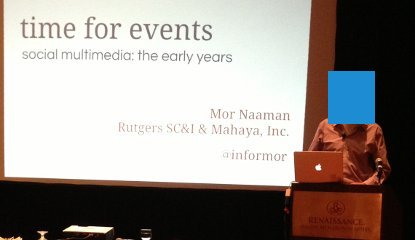
\includegraphics[width=\textwidth]{media/chapter1/icmr-keynote-2-hidden.jpg}
% \caption{Who is in this photo?}
% \label{fig:example-icmr-hidden}
% \end{minipage}
% \hspace{0.5cm}
% \begin{minipage}[b]{0.45\linewidth}
% \centering
% 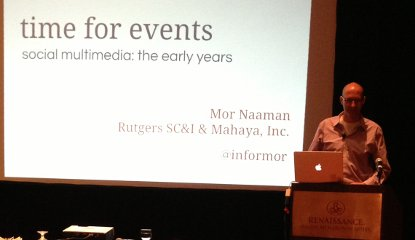
\includegraphics[width=\textwidth]{media/chapter1/icmr-keynote-2-show.jpg}
% \caption{Mor Naaman at ICMR.}
% \label{fig:example-icmr-show}
% \end{minipage}
% \end{figure}

\chapter{What is Context?}

This chapter describes what we mean by `Context' and `Context-Awareness'. We look at the previous definitions and usages of these terms, and propose why these are lacking for the purposes of this dissertation. As we go through each definition, we will pick out the most relevant parts to form the ground for the context framework introduced in this and developed in later chapters.

\section{Previous Definitons}

The earliest study on context was done by Bill Schilit in 1994, and reported in their paper [CITE]. The focus in this study was how to build software in dynamic environments. The dynamics of the environments were largely due to people requiring computational services, the modality of request (through a mobile device or through a workstation), and the environment of the device (are there cameras and projectors nearby if the task requires video conferencing?). This software-centric view of context highlights the importance of two things. One, context is always described with respect to an object. In this case it is the software which runs on processors distributed in a real world environment. Second, context is used to determine how this object interacts with events and entities near it? For example, Schilit uses the example that a workstation should automatically load his favorite text editor when he approaches it; and an rooster music sample must be played whenever fresh coffee is prepared. Both very different and precise interactions even though they might share common background (environment or participating entities). We would not expect a text editor to be shown when coffee is prepared, and the rooster music to be played when an employee walks to a workstation.

In his seminal paper, Anind Dey [CITE] describes context \textit{as any information that can be used to characterize the situation of an entity. An entity is a person, place or object that is considered relevant to the interaction between a user and an application, including the user and applications themselves.} He proceeds to explain this definition with the example of an ``indoor mobile tour", arguing that there are there are two additional pieces of information which can be used: \textit{weather} and \textit{presence of other people}. if the user is present with his friends, they might visist sites that are of interest to everybody. There the presence of other people is important context. Because the tour is indoor, weather does not affect the application. It is true that the weather has no direct affect on the application but what about the following scenarios:

\begin{itemize}
\item Could we use the weather information to serve different drinks in the cafeteria? On a cold day, placing the hot chocolate kiosk next to the entrance and the ice cream kiosk closer on a warmer day might boost some sales? And add to the overall experience of the tourists?
\item If the tour is similar to Alcatraz, where a ferry ride takes people to the island, and back from it, a storm brewing in the ocean could lead to disrputed ferry services. Should the application warn its users who are liesurely touring at this time? Or should they continue the tour at the same pace, miss the last ferry and spend the night at Alcatraz? After all, accommodation is not a problem.
\end{itemize}

They then proceed to define Context-Aware computing as follows: \textit{A system is context-aware if it uses context to provide relevant information and/or services to the user, where relevancy depends on the user's tasks}. But, we need to ask ourselves why a system which uses this ``additional information" should be considered a context-aware system. There are numerous system which simply would consider these ``additional information" as regular inputs. What is the different between a system which takes in these inputs as processes them as regular data, and one which processes them as context?

Karen Henricksen [CITE] makes the following interesting observation about context: Context information exhibits a range of temporal characteristics. Some context information can be static, for example the attributes of people using a system (for example, the sex of a person). But a large amount of information is dynamic. For example, relations change between people, location and events progress between moments. There is no straightforward way to obtain this dynamic information other than through sensors. But, such a approach tightly couples the application logic to the types of sensors used, and requires the system to convert the input data to usable representations. For example, the application might explicit modules to convert GPS coordinates to readable addresses. The problem with such an approach is that there are many ad-hoc modules built to tackle the sensors, and therefore causing the context-awareness to be tied to a specific application.

More recently, Vaninha Vieira [CITE] uses a knowledge centric view of context to design their context sensitive system, Cemantika. Vaninha defines a contextual element as any piece of data or information which can be used to characterize an entity in an application domain, whereas the context of an interaction between an agent and an application is the set of instantiated contextual elements that are necessary to support the task at hand. Context awareness, for them, is to explicitly change the task which the system is carrying out. For this they explictly model the \textit{context sources} which includes heterogenous and  external sources like sensors, user dialog interfaces and databases. This allows the various processes to operate independently of the type of sources. It should be noted that the use of ontologies is describing knowledge and context sources is becoming increasingly popular. A more listing of relevant work is provided in chapter 3. \textbf{This paves the way for us to bring in the notion of types of information}.

Let us extend the tour guide example to demonstrate the different properties of context. In this extension, we assume that this is the tour guide software to manage a visitor's experience at the Alcatraz Island, San Francisco. The visitor is allowed to walk through the exhibits as s/he pleases, with the tour guide headset providing explanations on the current exhibit, by sensing the current location. The explanations provided are such that they take into consideration what the visitor has already seen at the prison. For example, if the current location requires knowledge of an event which happened at a different section of the prison, then it must not be told. The application must also ensure that all visitors make it to a ferry ride before the last one departs for the day. If there is any problem in that respect, it must present the appropriate data which informs the visitor on the reason for the problem. Since this application knows where every visitor is at a given time, it must ensure that some sections of the Island do not get more crowded that the others. It should either slow down or move the visitors faster if the number of people in a section are increased beyond a particular threshold.

Let's assume that the Island is divided into sections, each of which contains a person counter sensor. The counter sensor can be queried to determine how many people are present in the section. Each visitor carries a handheld device which is capable of sensing its location, and proximity to an exhibit. The ferry maintains a schedule, which is read by the system to make decisions. If there is a problem with the ferry, a maintenance schedule which can be queried to check for any damages to the ferry. We also assume we have access to a local weather channel to check for sudden changes in the weather which might affect the ferry.

When a visitors enters the museum, all sensors are contributing towards the context of the visitor. The person counters are being queried to decide which section the user should move to next, the previous locations are used to form coherent explanations at each new stop. The ferry schedule is checked to make sure there are no disruptions along the way. But what happens when the visitor has finished seeing all the exhibits? We can now ignore all the previous locations, and traffic situation at the different sections. Even though these sensors are in the proximity of the visitor, they are no longer needed. And therefore, contribute no useful context. We can also say \textbf{that the relationships between the visitor, and his environment has changed through time}. Thus, it holds to say that the exact configuration of relationships, at that instant of time, is pivotal in deciding what real world information contributes to context, and what is unecessary.

Relationships can be of different types. They can be simple labels like \texttt{friend-of} signifying a social relationship. Or they can more actionable like \texttt{located-at}, which relates a person to a particular location, and therefore causes a particular audio stream to play through the handheld device. This relation is not just a label, it imposes constraints on the properties of objects which it relates. Here, the spatial attributes of the the person and the exhibit must match if they are being related through a \texttt{located-at} attribute. In this dissertation, we will see that such relations, which impose such property constraints are critical in algorithmically determining which information is relevant context.

We define context of a given object at a particular time as \textbf{``the real world information which can be related to the object directly or indirectly through a known set of relationships''}. Context-awareness of a system is its \textbf{``ability to explore different types of information to identify context relevant to the objects in its ecosystem, and using this additional knowledge to reduce the complexity of a given task''}.

\section{Properties of Context}

\subsection{Object Specificity}
Context is always specified with respect to a real world object. This object must be uniquely identifiable in the computational system, and must be an instance of one of the known classes. This object must have some real world attributes. For example, if the object is an event, then the interval during which it occurs, and location of occurence are two real world attributes.

\subsection{Relation Centric View}
We believe that any context is any event or entity which can be \textit{related} to the variables in a problem. It must be noted that focus has now shifted from finding objects which are of a specific type, and that to objects (of any type), but related to the problem variables through specific relationship types.

\subsection{Temporal Relevance}
The relations between problem variables and the context objects must be temporal in nature. There are two advantages to this. First, this allows us to associate different context objects (possibly of different types) to different instances of the problem. Second, real world relations are always temporal in nature. By explicitly modeling time in our definition of context, we are able to incorporate a majority of real world relations, which are very crucial in real world applications.

\subsection{Dynamic Linking}
When a problem uses a fixed set of context objects for all instances, we refer to it as static linking. But here argument would be -- why call it context? and not just a problem which uses an additional set of variables. In this dissertation, we believe that context must be \textbf{dynamically linked} to the problem variables. This follows from the above two points. For example, tagging faces in photos cannot restrict the search space to be just friends of the user on Facebook. 

In summary, we can say that context is any information which can be dynamically related to information present in the given problem, under the accepted spatio-temporal constraints.

\subsection{Context-Awareness}
Given the above properties of context, we define a system which is context aware as one, which when given access to different sources of additional information, has the capability to select information to reduce the complexity of the original problem.

In this dissertation, we will see one such way of selecting such information for a specific face tagging application. In this work, we use event semantics and sources to specify our relations and context respectively.

Also, context has been used in many non-real world problems. For instance, in natural language processing [CITE], ranking pages of the web [CITE-pagerank], entity resolution [CITE], face clustering [CITE] and therefore it must not mean that contextual techniques must apply only to real world problems. For the purposes of this dissertation, we ignore the application of context in such problems.

\section{Parallels}
In this section, we look at how context awareness has explained many of the long standing problems in different communities. We will start with an anecdotal example, and move to more elaborate examples which demonstrate how to reason in real world problems. The reason for this section is to justify the need for modeling many different types of real world information, which is a pre-requisite for employing context in the way it is justified above. Do we really need such large models? The sections below 

\subsection{Black Swans}
In his widely acclaimed book, The Black Swan, Nassim Nicholas Taleb presents many arguments against solely relying on prediction based techniques. Citing examples from stock markets to clinical psychology trials he presents the case that historical evidence is insufficient to position oneself in the future. 

His example of a turkey brings to light an interesting point ``Consider a turkey that is fed every day. Every single feeding will firm up the bird's belief that it is the general rule of life to be fed every day by friendly members of the human race ``looking out for its best interest''. On the afternoon of the Wednesday before Thanksgiving, something unexpected will happen to the turkey. It will incur a revision of belief.''

Any amount of prediction is futile in this case. Taleb shows the graph showing the belief of the turkey in mankind. How could the turkey protect itself, yet reaping the benefits of the food given to it? 

From the standpoint of the turkey, the Wednesday event is a Black Swan event. But from the standpoint of the butcher, it is not, since its occurrence is not unexpected.

The simple example shows how new objects bring with them different semantics. And highlights that object relations can be disrupted heavily with even the slight change in relations. The second thing it shows is the need for awareness in the turkey to ``look-out'' for potential causes of harm. This action of being context-awareness is criticial in any real world systems.

Figure shows how the turkey can navigate to various sources to learn how human beings behave. humans ..to.. festivals ..to.. thanksgiving ..to.. role of turkey in thanksgiving ..to.. butcher's profession.

\subsection{Context in History}
Historians love context. Almost all their works heavily rely on finding interesting events in a particular timeframe which can explain the reasons. In his book, Guns, Germs and Steel, Jared Diamond argues the need to understand specific environmental diversities, and use them to reason why history happened the way it did. We are familiar with the conquest story of the Inca emperor Atahuallpa by the Spanish conquistador Francisco Pizzaro at Cajamarca, Peru in 1532. Historians attribute the success of Pizzaro to better Spanish ammunition and warfare techniques. But the more interesting question is \textit{Why was Pizzaro at Cajamarca conquering the Incas, and not Atahuallpa crossing the Atlantic conquering Spain?}. How did South Americans evolve so different from Europeans? The answer, it turns out, lies in the environment.

Diamond shows the various steps in a flowchart similar to [FIGURE]. Lets see how he arrived at this. For a conquest of the Americans, the Europeans needed strong political and economic and  structure, which means separate organizations devoted to monitoring these. The South Americans lacked a political structure. The society consisted of the high ranking chiefs who were treated as Gods, and were the only people permitted to read and write. Everyone else was engaged in food production. In a war, the ability of the Europeans to communicate precise information through the written word was a crucial advantage.

\textbf{Why did the Europeans form such a stratified society, and not the South Americans?} The majority of the south americans were concerned about procuring food for the next day. Food production systems in Europe reached a critical peak, because of which they developed technology for storing food. Because day-to-day food was no longer a concern, a significant section of the population now was ``free'' to indulge in other activities. This led to development of art, policital, military units, economic systems, which in turn evolved each.

\textbf{Why did food production reach an all time high in Europe and not in South America?} The reason lies in three environmental factors: the soil, flora and fauna of the area and over a larger time span. Europe and Asia has been home to a more diverse set of animals and plans. Since 6000B.C., farmers and animals of the area were able to choose from this bigger variety of plants, and evolve them over thousands of years to form better crops. Big mammals like Cows, Bulls were found in plenty in Europe and Asia. This led to much higher yields than tilling the soil by hand or manually. The role of a larger set of animals in the area is interesting too. Over the years, Europeans have domesticated most of the animals than people from any part of the world (owing to the diversity, animal behavior and the abilities of the animal). For example, there is no point in domesticating an elephant, as it takes 14-15 years to reach adulthood and be of use. Animals like Rhinos can be excellent farm animals owing to their strengths, but are very hard to tame. Areas like Africa were rich in elephants and rhinos but America lacked those too, and both these continents lacked important livestock like cows, bulls and sheep.

\textbf{Finally, why did biodiversity emerge in Europe/Asia, and not in the Americas or Africa?} Thousands of years ago, the biggest deterrent in sustaining life was the climate. People lived nomadic lifestyles which came in contact with different weather, and acclimatizing to it required almost a reboot of their knowledge, environmental know-how and customs. Now, lets take a look at the map of the world, shown in [FIGURE] -- what do we see? Europe and Asia span longitudinally, whereas Americas and Africa extend along Earth's latitude. What is the biggest advantage this offers Eurasians? When they moved from place to place, the structure of their continent allowed them to move to places with \textbf{similar weather}. This allowed them to move to different regions and enjoy the same weather, grow similar crops and domesticate the same animals. But people in Africa or America had to move out of their comfort zone, and move to area containing different weather and biodiversity, and had to redo everything from scratch. 

There is also this idea that frequent learning cultures had to deal with more complexities of the world, and could rely less on objective knowledge, and therefore led to creation of religious following. The colored map shows the amount of religion in different countries:

% http://pocketcultures.com/topicsoftheworld/files/2009/06/map-importance-of-religion-by-country.png

% http://en.wikipedia.org/wiki/File:Religion_in_the_world.PNG

Diamond's book is an exploration of the broadest pattern of history. What it tells us is that explicit modeling of real world objects with their native properties is extremely important in reasoning about the world.

\subsection{The Gaia Hypothesis}
Charles Darwin's work describes how living being have evolved over billions on years. But it does not answer the question -- how does life sustain itself on Earth? It turns out that the few billion years of life we have had is too little to let life have grown randomly, and just let natural selection determine who succeeds. There had to be bigger factors which let life sustain and grow in specific ways.

One of the theories proposed in the 1970s is commonly known as the Gaia Theory. Proposed by James Lovelock and Lynn Margulis, it proposes the presence of feedback loops to explain the sustanence of life. Their argument is that for life to sustain, the amount of carbon dioxide in the atmosphere must not exceed a certain threshold. But who keeps this in check? How has the amount of CO2 in the atmosphere been almost constant for the last millions of years. Their reasoning is as follows:

The Earth's volcanoes have spewed out huge amounts of carbon dioxide for millions of years. Plant and animals recycle massive amounts of CO2 in the process of photosynthesis, respiration and decay. According to the Gaia theory, the excess of CO2 is recycled is removed and recycled by a vast feedback loop, which involves rock weathering as a key ingredient. In the process of rock weathering, rocks, rainwater and CO2 form chemicals known as carbonates which are taken out of the atomosphere and bound in liquid solutions. It turns out that soil bacteria vastly increases the rate of rock weathering. The carbonates are then washed down where tiny algae invisble to the naked eye, absorb them and use them to make shells of chalk. So the CO2 that was in the atmosphere has now ended up in the shells of those minute algae. In addition, ocean algae also absorb $CO_2$ from the ocean.  

When the algae die their shells are then washed down into the ocean, where they form sediments of limestone. Limestone is very heavy, and gradually sinks into the mantle of the earth. Eventually, some of the CO2 is released back to the atomsphere by volcanoes. The entire cycle -- linking volcanoes to rock weathering, to soil bacteria, to oceanic algae, to limestone sediments, and back to volcanoes -- acts as a feedback loop which regulates the Earth's temperature. As the sun gets hotter, the bacteria in the soil get hotter, and more CO2 is removed from the atmosphere and sent to the ocean, thus cooling the planet.

This remarkable explanation involves rocks, bacteria and ocean dynamics and the even the sun to explain how the earth's temperature is regulated. By studying one or more objects in isolation makes the analysis far from complete. More interestingly, the relations between the objects are very precise, involving biochemical reactions and have very precise definitions.

\subsection{Significance}

\section{Context for Personal Photos}
Our justification for the use of context begins with the statement: \textit{For a given user, the correctness of face tags for a photograph containing people she has never met is undefined}. This observation prepares us to understand what context is, and how contextual reasoning assists in tagging photos. The description of any problem domain requires a set of abstract data types, and a model of how these types are related to each other. We \textbf{define} contextual types as those which are semantically different from these data types, but can be directly or indirectly related to them via an extended model which encapsulates the original one. Contextual reasoning assists in the following two ways. \textbf{First}, contextual data restricts the number of people who might appear in the photographs. We can also argue that all the personal data of a user (her profile on Facebook, LinkedIn, email exchanges, phone call logs) provides a reasonable estimate of all these people who might appear in her photos. \textbf{Second}, by reasoning on abstractions in the contextual domain, we can infer conclusions on the original problem. We exploit this property to develop our algorithm in the later sections. Though CueNet can be applied to a variety of recognition problems, we focus on tagging people in personal photos for concreteness, where, the image and person tag form the abstractions in the problem domain. The types used in the contextual domain, but not limited to, are the following:

\begin{itemize}
\item \textbf{Events}: includes description of events like conferences, parties, trips or weddings, and their structure (for example, what kind of sessions, talks and keynotes are occurring within a particular conference).
\item \textbf{Social Relationships}: information about a user's social graph, people whom she corresponds with using email and other messaging services.
\item \textbf{Geographical Proximity}: various tools like Facebook Places, Google Latitude or Foursquare provide information about where people are at a given time.
\end{itemize}

The above classes of contextual data can be obtained from a variety of data sources. Examples of data sources range from mobile phone call logs and email conversations to Facebook messages to a listing of public events at upcoming.com. We classify sources into the following types:

\begin{itemize}
\item \textbf{Personal Data Sources}: include all sources which provide details about the particular user whose photo is to be tagged. Some common examples of personal data sources include Google Calendar, Email and Facebook profile and social graph.
\item \textbf{Social Data Sources}: include all sources which provide contextual information about a user's friends and colleagues. For example, LinkedIn, Facebook and DBLP are some of the commonly used websites with different types of social graphs.
\item \textbf{Public Data Sources}: include all sources which provide information about public organizations (like restaurants, points of interest or football stadiums) or about public events (like fairs, concerts or sports games).
\end{itemize}

Social and public data sources are enormous in size, containing information about billions of events and entities. Trying to use them directly will lead to scalability problems faced by face recognition and verification techniques. But, by using personal data, we can discover which parts of social and public sources are more relevant. For example, if a photo was taken at San Francisco, CA (where the user lives) his family in China is less relevant. Thus, the role of personal information is twofold. \textbf{Firstly}, it provides contextual information regarding the photo. \textbf{Secondly}, it acts as a bridge to connect to social and public data sources to discover interesting people connected to the user who might be present in the event and therefore, the photo.

At this point we will mention the \textbf{temporal relevance} property of a data source. Given a stream of photos taken during a time interval, the source which contributed interesting context for a photo might not be equally useful for the one appearing next. This is because sources tend to focus on a specific set of event types or relationship types, and the two photos might be captured in different events or contains persons with whom the user maintains relations through different sources. For example, two photos taken at a conference might contain a user's friends in the first, but with advisers of these friends in the next. The friends might interact with the user through a social network, but their advisers might not. By using a source like DBLP, the relations between the adviser and friends can be discovered. We say that the temporal relevance of these context sources is \textbf{\textit{low}}. This requirement will play an important role in the design of our framework, as now, sources are not hardwired to photo, but instead need to be discovered gradually.

conclusion: by using events we get dynamic linking, temporal relevance and real world integration.



%\subsection{Zeno's Paradox}
% \textit{In the paradox of Achilles and the Tortoise, Achilles is in a footrace with the tortoise. Achilles allows the tortoise a head start of 100 metres, for example. If we suppose that each racer starts running at some constant speed (one very fast and one very slow), then after some finite time, Achilles will have run 100 metres, bringing him to the tortoise's starting point. During this time, the tortoise has run a much shorter distance, say, 10 metres. It will then take Achilles some further time to run that distance, by which time the tortoise will have advanced farther; and then more time still to reach this third point, while the tortoise moves ahead. Thus, whenever Achilles reaches somewhere the tortoise has been, he still has farther to go. Therefore, because there are an infinite number of points Achilles must reach where the tortoise has already been, he can never overtake the tortoise.}

% How can achilles win? Idea: Ignoring a variable can make a process very hard to explain. Different variables work together holistically. In this case, it is time. Just by bringing it into the same picture the problem becomes tractable.

\chapter{Related Work}

In this chapter, we will look at the state-of-the-art understanding of different topics presented in a variety of areas, which context relies on. These include techniques to annotate photos using image features, techniques to represent knowledge in ontologies, techniques to query data from a variety of sources.

\section{Photos and Annotation}

Kindberg \cite{kindberg2005ubiquitous} conducted a study on multiple subjects to analyze photo capture behavior. Specifically, they were trying to understand the different motivations for people to take photos. They found two main motivations -- \textit{affective} and \textit{functional}. A significant number of photos are captured to enrich a shared experience, or to share an experience with absent members like friends or family. Much lower, but a significant amount of photos were taken to share photos who were present at the event. Their study shows that photos are mostly used in social context, and lesser in personal context. Ames \cite{ames2007we} and Frohlich \cite{frohlich2002requirements} independently describe a survey conducted to study motivations for people to tag their photos. They noticed two broad motivations: Organization of photos and Communication with photos. Almost orthogonal to the applications observed by Kindberg, Ames and Frolich are brave new world applications for photography described in \cite{gemmell2002mylifebits, dumais2003stuff}, where life logs were collected in the form of photos, emails, document scans and stored in SQL Server database, and photos were retrieved using SQL queries. The photo content was tagged by the user in this case. The annotated photos are used exclusively for personal \textit{feedback} to improve quality of life. The medical advantages of collecting photos to log personal health are becoming very well known \cite{bell2010total}.

\subsection{Spatio-Temporal Annotation}
Ever since its release in 1995, EXIF metadata, contained in JPEG photos, has been exploited to organize pictures. Almost all photo management applications use timestamps to order photos in an album, a concept which has also been studied in academia \cite{graham2002time, hailpern2011youpivot}. Apple's iPhoto is the most common example of using both time and space to organize personal photos. Naaman et al.\ have exploited GPS attributes to extract place and person information \cite{naaman2005leveraging, naaman2005identity}. Rattenbury \cite{rattenbury2009methods} devised techniques to find tags which describe events or places by analyzing their spatiotemporal usage patterns. Sinha \cite{sinha2008concept} and Boutell \cite{boutell2005beyond} have used EXIF metadata to predict concepts such as (Indoor, Outdoor, Portrait, Landscape) to further organize these photos. Boll \cite{boll2007semantics} is a very interesting work which aggregates textual and experiential content from web 2.0 communities about places using a set of predefined rules. These works motivate the need for adding annotations to improve the overall experience of viewing a collection of photos.

\subsection{Computer Vision}

The Computer Vision community has contributed extensive work in the area of detecting scenes \cite{xiao2010sun}, humans \cite{dalal2005histograms} or geo localization \cite{hays2008im2gps}. Here we will specifically look at the part of the computer vision research which is relevant to face tagging.

\textbf{Face Recognition}
The face recognition problem is one of the primary problems taken on by the computer vision community, the others being action, pose, gesture recognition and human detection. One of the earliest works on recognizing people in faces was attempted by Turk and Pentland in \cite{turk1991eigenfaces}. The essence of the technique put forward here was to extract useful features which can be represented mathematically and compared using some distance measures (such as euclidean, mahalanobis or cosine distance) to features in an image database. This contribution sparked a large interest in the community to find more meaningful and powerful features, which led to Fisherfaces \cite{belhumeur1997eigenfaces} and more recently, local binary pattern \cite{ahonen2006face} features. SIFT features have also been used to identify faces \cite{bicego2006use, geng2009sift, luo2007person}. One of the big difficulties of such feature-based representation is the scalability of the technique. It is now well known that with the increasing number of candidates, these distance based techniques provide in lower performance \cite{wu2004probability}. A quick alternative is to increase the dimensions in the features to allow for more diversity, but it has been proven that as the number of dimensions increase, the maximum distance between the two points reduces, and if the number of dimensions is as less as 32, the distance is almost negligible \cite{beyer1999nearest}. Effectively, for dimensions more than 32, the distance between all points can be considered very small, and the concept of `nearest-neighbour' loses its meaning. Thus, an pure feature based technique cannot be used to build large scale real world photo tagging frameworks.

\textbf{Face Verification}
More recently, face verification techniques have attracted a lot of attention in the computer vision community. One of the earliest efforts towards robust face verification was undertaken by Huang et al.\ in \cite{huang2007labeled}. They constructed and annotated a dataset of profile photos of celebrities taken in unrestricted environments. Previous datasets such as FRGC \cite{phillips2005overview}, BioID \cite{jesorsky2001robust} and the color FERET database \cite{phillips1998feret} were criticized to have photos taken at very constrained environments thereby reducing the complexity of the face tagging problem. But the techniques which worked on such photos could not duplicate their performance in real-world photos. Huang's database, commonly known as the \textit{Faces In the Wild} has allowed many researchers to implement various face verification technologies. A recent and important development on top of Huang's work is that of Neeraj Kumar et al.\ \cite{nk_attribute_classifiers}, where the confidence of presence or absence of facial attributes such as range, skin color, hair style, gender, eye color features are used to train various classifiers to ultimately test if two given faces are of the same person or not? The technique was able to achieve up to 85.29\% accuracy on the LFW dataset. More recently, Berg \cite{berg2012tom} increased this accuracy to 93\% by automatically finding distinguishing features.

The interesting perspective face verification brings forward is in its contract with co-existing components in a system. Whereas, face recognition works as a standalone component, face verification doesn't make this assumption, and allows external components to filter candidates. This systemic behavior of face verification will prove to be very useful in future systems.

\textbf{Probabilistic Techniques}
Both face verification and recognition techniques seen so far assume that none of the input photos contain any annotation. But what if this assumption could be relaxed? A large number of photos on Facebook, Flickr or Google+ are annotated. If we further assume that these partial annotations are mostly true, the label propagation technique by Cao et al.\ \cite{cao2008annotating} can be applied to annotate the rest of the dataset. This technique was tested on propagating concept based tags (such as beach, fun, dinner, yard) on personal photo datasets. Also, Barthelmess et al.\ extract semantic tags from noisy datasets containing discussions, speeches about a set of photos in question\cite{barthelmess2007toward}. 

\textbf{Miscellaneous Techniques}
Collaborative games also have been evaluated as a possible way to tag photos\cite{diakopoulos2007photoplay}. Systems like Picasa, iPhoto and \cite{graham2002time} organize photos based on time, GPS coordinates and sometimes faces in the photo. These attributes of the photo do not capture event semantics \cite{sawant2011automatic}. Events are a natural way of categorizing photo media. Events also allow large number of photos captured during a single event be organized hierarchically using subevents.

\section{Context}
The use of context in the sciences has been continuously increasing. It finds applications in various fields, starting from its use in holistic thinking to better understand biological and ecological phenomenon in \cite{capra1997web}, to associating the right external data to form coherent stories about economic phenomenon \cite{levitt2006freakonomics}, to associating plausible connections between history and geography in \cite{diamond1997guns}. The advances proposed in these works can be loosely characterized as ``utilizing external information" or ``out-of-the-box thinking". The reason they are included in this section is because of their common trait of relating multiple pieces of external data, to create coherent stories which allows the scientists to gain valuable insights into the problem they are solving.

\subsection{Uses in Computing}
In Computer Sciences, the main interest towards context has been largely from the Pervasive Computing community and the Human-Computer Interaction community. Their interpretation of the word context is mainly inspired from the definition set by Anind Dey \cite{dey2001understanding}, i.e. \emph{Context is any information which describes the situation of an entity}. The role of context in mobile computing has been studied in \cite{chen2000survey}. It shows the growing importance of contextual thinking in reasoning about networking problems in the mobile computing era. 

More recently, information retrieval communities are showing interest in context based representation of data and context-based techniques. One of the most important works in information retrieval is the PageRank algorithm \cite{page1999pagerank} developed by Google co-founders Larry Page and Sergey Brin in 1996. In this work, Page and Brin define context as the links between different web pages, and the anchor text of these links, and argued that this context is more descriptive of a page than the contents of the page itself. PageRank was derived by combining this insight with Jon Kleinberg's HITS \cite{kleinberg1999authoritative} algorithm.

\subsection{Definitions}
There are many definitions of the word context in academic works. Notable among them are those of Schilit \cite{schilit1994context}, Dey \cite{dey2001understanding}, Viera \cite{vieira2011designing}, Zimmermann \cite{zimmermann2007operational} and the work of Patrick Brezillon, a summary of which can be found in \cite{mostefaoui2004context}. One of the problems with the term Context is the overloaded use of it \cite{henricksen2002modeling}. To this effect, Brezillon compiled a list of 150 definitions, and did to this list what lots of scientists do with large collections of text -- text analysis using natural language processing techniques, and derived the essential components which should make up a holistic definition of context. Their conclusion as described in \cite{bazire2005understanding} was that \textit{context acts like a set of constraints that influence the behavior of a system (a user or a computer) embedded in a given task}. In spite of this promising ``big-data" analysis, many questions are unanswered. For example, is context internal or external? Is it a phenomenon or an organized network? To the best of my knowledge, there is no consensus on what is a good definition of this word, and what are the general principles that one can be find a context-aware system.

\subsection{Role in Photo Annotation}
In \cite{dumitrescu2009context} Dumitrescu and Santini argue that ``images are a node in a complex network of signification that goes beyond their content and includes other form of textuality that go around them, as well as the cultural practices of the community that creates or receives images". Such philosophies became more commonplace after the web went contextual with PageRank. Image retrieval, specifically, obtained a remarkable opportunity to index and rank images on the web by using the textual content which accompanies it \cite{chen2001web, frankel1996webseer}. Later, with Flickr the amount of user contributed tags has resulted in gigantic datasets which allow researchers to train sophisticated machine learning models to produce one or more relevant tags \cite{brachmann2013feature, li2013geo, liu2013heterogeneous}. Some of early advocates of using external context to annotate photos are \cite{datta2008image, jain2010content}. Context information and image features are used in conjunction by \cite{o2009context, cao2008annotating, boutell2005beyond, cao2008eventscene} identify tags. The semantic web community is using linked data technologies to annotate and query photographs \cite{monaghan2006automating, nowack2006confoto}. 

\subsection{Modeling Context}
Context is represented using three components: knowledge, external context and proceduralized context by \cite{brezillon2003context}. These ideas are represented using a contextual graph (CxG) representation of knowledge and reasoning. Henricksen et al.\ also use a graphical notation to represent their context. The former approach uses the graph to model the flow of reasoning between different objects within an environment, whereas the latter approach uses graph to only represent the various objects and their inter-relationships. Their modeling framework allows representation of static and dynamic associations, which is very critical in modeling real world relationships. For our work, we rely on primitives like the one mentioned in this framework as well as event relations mentioned in \cite{gupta2011managing}. \cite{reignier2007context} presents a technique to transform contextual graphs similar to concrete situation handling implementation using Petri Nets. \cite{hong2009context} presents a detail survey of various other context-aware systems.

Probabilistic and statistical frameworks are used to incorporate context in problem solving too. One example of using a probabilistic framework is \cite{cao2008annotating}, where high confidence tags from a few contextual images are propagated to other images which were taken during the same event. \cite{stone2008autotagging} uses potential functions in conditional random fields to model social relations and photo co-occurrence strengths. More recently, Zhang \cite{zhang2013unified} used cues from photos like clothing, human attributes like face complexion or gender, people co-occurrence and scene annotations to cluster similar faces in photos together.

\subsection{Industrial Momentum}
The tech industry is immersed in the so-called ``big-data" revolution. In order to make sense of such large collections of data, context is becoming increasingly popular. One of the biggest works in this area is the blog and upcoming book ``Age of Context" by Robert Scoble and Shel Israel\footnote{http://scobleizer.com/2013/02/12/a-new-way-to-fund-a-books-development-sponsors-heres-ours/}. The reasons for this interest is cited on the increasing number of smartphones and sensors, personal and public. The increasing number of wearable devices like Google Glass, Oakley AirWave Goggles, Plantronics, Smith I/O Recon Heads-up Display, FitBit, Basis Watches, Nike FuelBand  and Jawbone Up's personal health/activity monitoring gadget. The continuously increasing social data from companies like Facebook, Twitter, Flickr, Instagram and Pinterest, and information about locations through services like Foursquare, Google/Bing Maps, Waze and Factual. Lesser known startups like Tempo and Cueup (formerly Greplin) which are entirely focused on using personal contextual information to simplify otherwise very hard problems.

\section{Knowledge Representation}

\begin{figure}[ht]
\begin{minipage}[b]{0.45\linewidth}
\centering
\frame{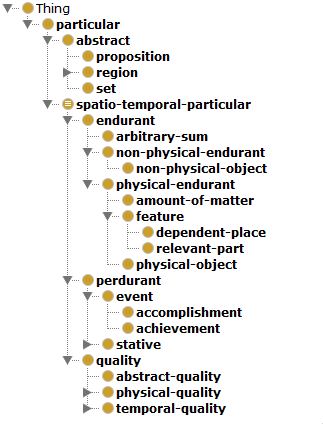
\includegraphics[width=\textwidth]{media/chapter3/dolce-taxonomy}}
\end{minipage}
\hspace{0.5cm}
\begin{minipage}[b]{0.45\linewidth}
\centering
\frame{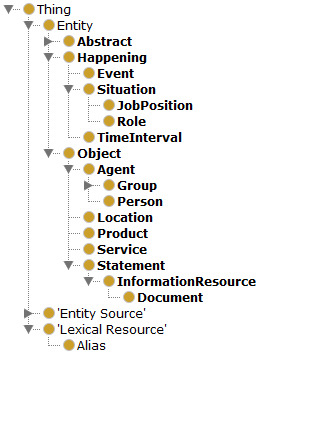
\includegraphics[width=\textwidth]{media/chapter3/proton-taxonomy}}
\end{minipage}
\caption{Dolce and Proton Class Hierarchies}
\label{fig:ontology-hierarchies}
\end{figure}

In our work, we use ontologies to model key pieces of knowledge. This includes the type of objects and relationships they are expected to have. OWL is the current standard language in authoring ontologies. The current standard being OWL 2.0. The majority of work, related to this dissertation, is in utilizing ontologies have been in the data integration domain \cite{smith2007obo, noy2004semantic, astakhov2005data}. We utilize some of the features of the declarative mapping language \cite{dou2005ontology} to express the structure of relations stored in various data sources. Specifically, we use the s-expression like syntax to declare the relations and the mapping axioms which relate items in the expression to objects in our ontology. SPARQL \cite{prud2008sparql} is the current standard for querying RDF documents. The event and entity discover queries generated by the discovery algorithm in the next chapter are generated using SPARQL templates.

We use the terminologies followed in upper level ontologies. Figure \ref{fig:ontology-hierarchies} shows the class hierarchies for the Dolce Upper Ontology (on the left) and the Proton Top Level Ontology (on the right). Similar to these taxonomies, we will use the term `entities' to collectively refer to all real-world events and objects. Events, are perdurants, and have temporal or spatial parts. Events in our context discovery will include Academic Conferences, Concerts, Photo-Capture Events or Meetings. Objects, such as Persons, on the other hand, are uniquely identifiable wholes. They do not need temporal or spatial attributes for their description. It must be noted that we extend the DOLCE-Lite upper ontology to construct our knowledge base for CueNet.

% Before looking at the different views on context, its advisable to distinguish between `objects' and `entities'. We use the word `Object' to collectively refer to events and entities. The term `object' has been used in literature to refer to things which have no temporal properties. But, in our discussion, an `object' could imply an event which exhibits temporal properties. An entity includes persons, places or organizations present in the world which do not temporal descriptors for their unique representation, for example `Starbucks, UC Irvine', `The Eiffel Tower, Paris, France', or organizations, for example `Google Inc', `Royal Society of London'. Effectively, they are objects which do not need temporal descriptors. Events, on the other hand, are objects which rely on temporal attributes.

% \begin{figure}[h]
% \centering
% 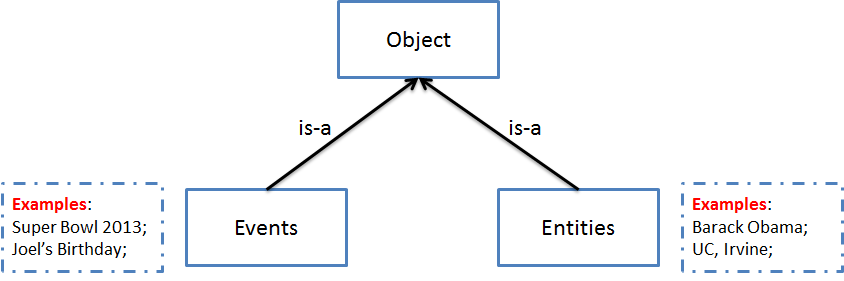
\includegraphics[width=0.6\textwidth]{media/chapter1/terminology.png}
% \caption{Objects, Events and Entities.}
% \label{fig:terminology}
% \end{figure}

\chapter{Context Discovery Framework}

In this chapter, we shall look at the functional parts of the CueNet framework: a \textit{data integration module} to model and query the various data sources and sensors, a \textit{discovery algorithm} to construct queries agnostic to what to the sources themselves, a \textit{knowledge representation module} to store relationships about the various real world objects, and finally how these parts integrate with a \textit{face verification algorithm}, which predicts if a person is present in a photo or not.

\section{Pruning Search Spaces with CueNet}

Automatic media annotation algorithms essentially assign one or more labels from a search space to a given input image. Figure \ref{fig:with-without-cuenet} shows the various approaches of constructing such a search space for such an algorithm. The traditional approach is shown in \ref{fig:with-without-cuenet}(a). These spaces were limited to a set of labels chosen by an expert, with no way of pruning the search space in case it got very large. The focus was instead on extracting the best features from images, to obtain high overall classification accuracy\cite{turk1991eigenfaces}.

\begin{figure}[t]
\centering
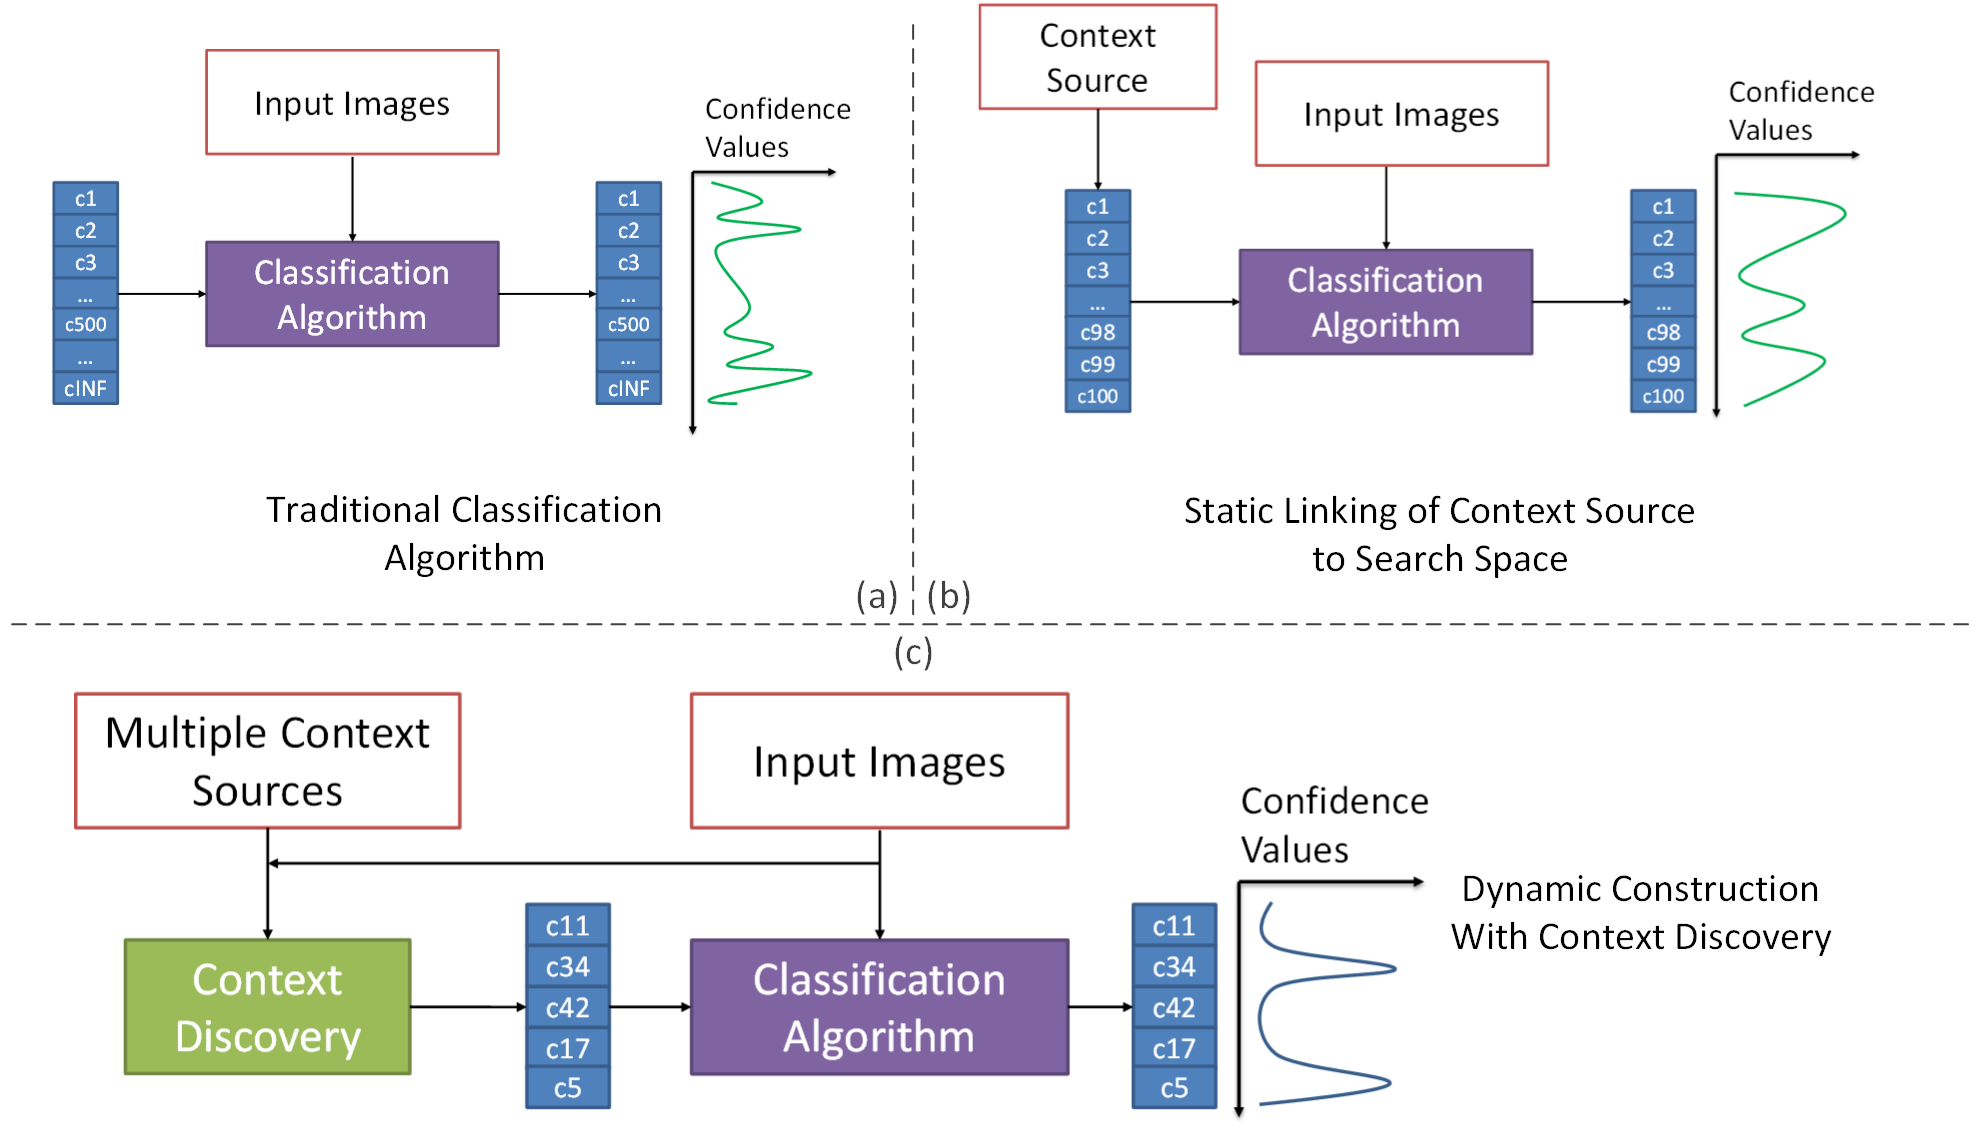
\includegraphics[width=0.95\textwidth]{media/with-without-cuenet-2.png}
\caption{The different approaches in search space construction for a multimedia annotation problem. A traditional classifier setup is shown in (a) where the search space candidates are manually specified. Context is used to generate large static search spaces in (b). The desired framework is shown in (c), which aims to produce small search spaces with many correct annotations.}
\label{fig:with-without-cuenet}
\end{figure}

With the popularity of global social networks and proliferation of mobile phones, information about people, their social connections and day-to-day activities are becoming available at a very large scale. The web provides an open platform for documenting many real world events like conferences, weather events and sports games. With such context sources, the search space construction is being delegated to one or a few sources \cite{henter2012tag, li2012fusing, naaman2005identity, o2009context,  stone2008autotagging} (figure \ref{fig:with-without-cuenet}(b)). These approaches rely on a single \textit{type} of context. For example, time and location information or social network information from Facebook to solve the face recognition problem. We refer to such a direct dependency between the search space and a data source as \textbf{static linking}. Although these systems are meritorious in their own right, they suffer from the following drawbacks: they do not employ multiple sources, and therefore the \textbf{relations} between them. By realizing that these sources are interconnected in their own way, we are able to treat the entire source topology as a network. Our intuition in this work is to navigate this network to progressively discover the search space for a given media annotation problem. Figure \ref{fig:with-without-cuenet}(c) shows how context discovery can provide substantially smaller search spaces for a set of images, which contain a large number of correct tags. A small search space with large number of true positives provides the ideal ground for a classification algorithm to exhibit superior performance.

\textbf{The CueNet framework}, provides access to multiple data sources containing event, social, and geographical information through a unified query interface to extract information from them. CueNet encapsulates our \textbf{Context Discovery Algorithm}, which utilizes the query interface to discover the most relevant search space for a media annotation problem. To ensure a hands-on discussion, we show the use of context discovery in a real world application: face tagging in personal photos. As a case study, we will attempt to tag photos taken at conference events by different users. These photos could contain friends, colleagues, speakers giving very interesting talks, or newly found acquaintances (who are not yet connected to the user through any social network). This makes the conference photos particularly interesting because no single source can provide all the necessary information. It emphasizes the need to utilize multiple sources in a meaningful way.

\begin{figure}[t]
\centering
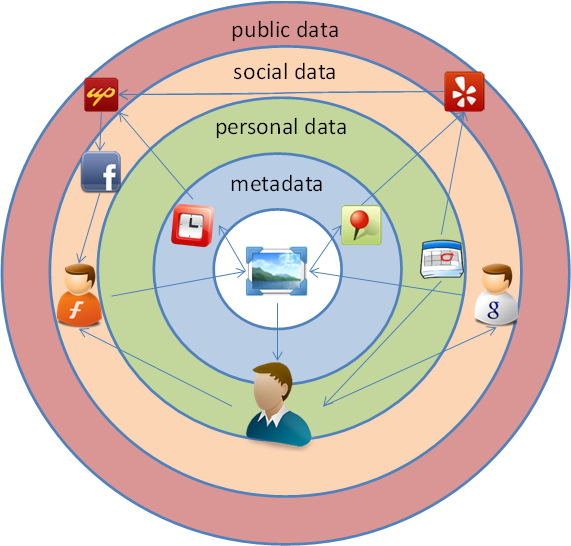
\includegraphics[width=0.65\textwidth]{media/prog-discovery.png}
\caption{Navigation of a discovery algorithm between various data sources.}
\label{fig:prog-discovery}
\end{figure}

Here is an \textbf{example} to illustrate CueNet's discovery process. Let's suppose that Joe takes a photo with a camera that records time and GPS in the photo's EXIF header. Additionally, Joe has two friends. One with whom he interacts on Google+, and the other using Facebook. The framework checks if either of them have any interesting event information pertaining to this time and location. We find that the friend on Google+ left a calendar entry describing an event (a title, time interval and name of the place). The entry also marks Joe as a participant. In order to determine the category of the place, the framework uses Yelp.com with the name and GPS location to find whether it is a restaurant, sports stadium or an apartment complex. If the location of the event was a sports stadium, it navigates to upcoming.com to check what event was occurring here at this time. If a football game or a music concert was taking place at the stadium, we look at Facebook to see if the friend ``Likes" the sports team or music band. By traversing the different data sources in this fashion, the number of people, who could potentially appear in Joe's photograph, was incrementally built up, rather than simply reverting to everyone on his social network or people who could be in the area where the photograph was taken. We refer to such navigation between different data sources to identify relevant contextual information as \textbf{progressive discovery}. The salient feature of CueNet is to be able to progressively discover events, and their associated properties, from the different data sources and relate them to the photo capture event. We argue that given this structure and relations between the various events, CueNet can make assertions about the presence of a person in the photograph. Once candidates have been identified by CueNet, they are passed to the face tagging algorithm (as in \cite{facever_pami2010}), which can perform very well as their search space is limited to two candidates.

Figure \ref{fig:cuenet-arch} shows the different components of the CueNet framework. The Ontological \textbf{Event Models} specify various event and entity classes, and the different relations between them. These declared types are used to define the \textbf{Data Sources} which provides access to different types of contextual data. The \textbf{Person Verification Tools} consist of a database of people, their profile information and photos containing these people. When this module is presented with a candidate and the input photograph, it compares the features extracted from the candidate's photos and the input photo to find the confidence threshold. In this section, we describe each module, and how the context discovery algorithm utilizes them to accomplish its task.

\begin{figure}[t]
\centering
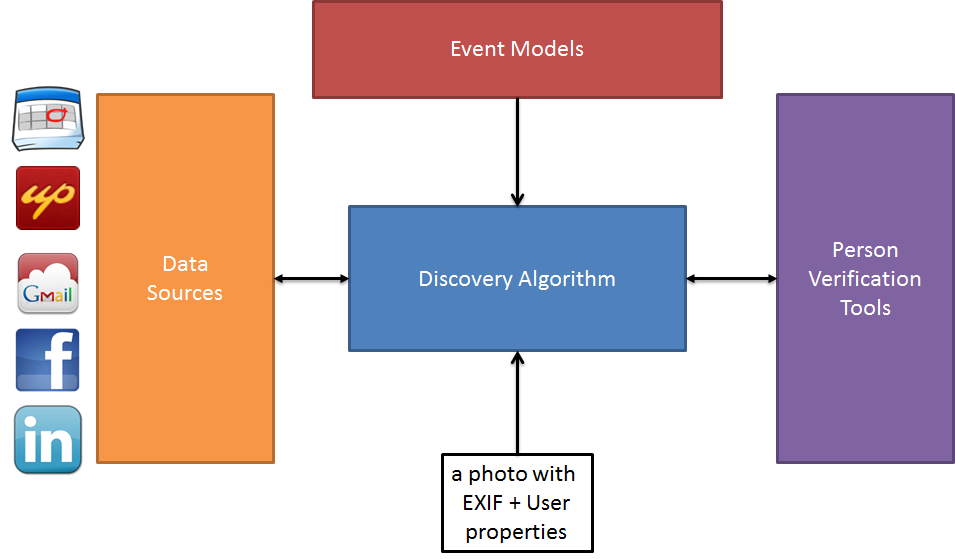
\includegraphics[width=0.9\textwidth]{media/cuenet-high-level-arch.png}
\caption{The Conceptual Architecture of CueNet.}
\label{fig:cuenet-arch}
\end{figure}

\section{General Approach}
Figure \ref{fig:cuenet-arch} shows a high level architecture of CueNet. The major functional blocks consist of a data integration system (left), which provides a uniform query interface to a multitude of autonomous data sources, which may reside within an enterprise or on the World-Wide Web \cite{halevy2001answering}; a specification of model describing real-world knowledge in terms of objects and their relations, along with any axioms and constraints to be imposed on instance graphs (top); since we are assisting face tagging application, the final block (right) consists of a set of hooks to invoke appropriate face tagging algorithms by providing a set of candidate for the input photo. In this work, we shall assume verification semantics in such a tagging algorithm, where given an input photo and a candidate person, the algorithm returns true or false (with a confidence score). Face recognition models would have to be retrained when the candidate set changes. Also, as described in chapter 3, the state-of-the-art techniques for face verification perform much more reliably than their recognition counterparts. At the heart of CueNet, lies the context discovery algorithm. Given a photo the algorithm constructs a context network with all the known information. Using the knowlege base, the algorithm constructs queries to be executed on the interface provided by the data integration layer. Objects which are returned are merged into existing context network. New entities in the network are passed to the face tagging algorithm to check for their presence in the photo. If they are present, the context network is altered to reflect this fact. The execute-merge cycle is iteratively performed until all the faces are tagged, or the data integration module is unable to furnish any new data.

\section{Execution Trace}
In this section, we will trace the execution on two different photos, to see how the different modules interact to produce context networks, and how they are used to tag faces. The first example will be a relatively simpler one, requiring only 2 data sources, whereas the second photo will require multiple sources to sucessfully tag all photos.

\subsection{Simple Case}

Consider the photo shown in figure \ref{fig:stacktrace-simple-torsten-hidden}. For the purposes of this trace, we assume that we have access to the sources shown in figure \ref{fig:stacktrace-simple-sources} through the data integration module. Given, an input photo, the knowledge base is queried to find what other objects can be associated with an photo object. The KB stores the information that every photo consists of an EXIF header, which stores timestamp and location coordinates and a fact which states that every photo is owned by a user object, where \textbf{owner-of} is a relationship described in the KB. This knowledge is used to construct the context network shown in figure \ref{fig:exif-network}.

\begin{figure}[ht]
\begin{minipage}[b]{0.45\linewidth}
\centering
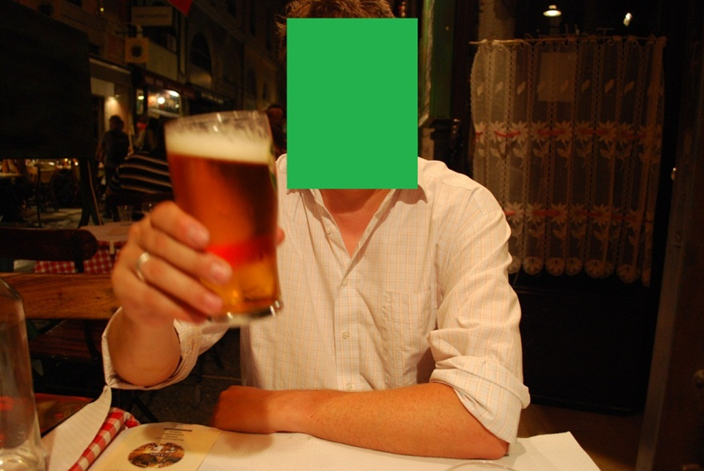
\includegraphics[width=\textwidth]{media/chapter4/stacktrace/torsten-hidden.png}
\caption{Input Photo.}
\label{fig:stacktrace-simple-torsten-hidden}
\end{minipage}
\hspace{0.5cm}
\begin{minipage}[b]{0.45\linewidth}
\centering

\includegraphics[width=\textwidth]{media/chapter4/stacktrace/sources.png}
\caption{Available Data Sources.}
\label{fig:stacktrace-simple-sources}
\end{minipage}
\end{figure}

\begin{figure}[h]
\centering
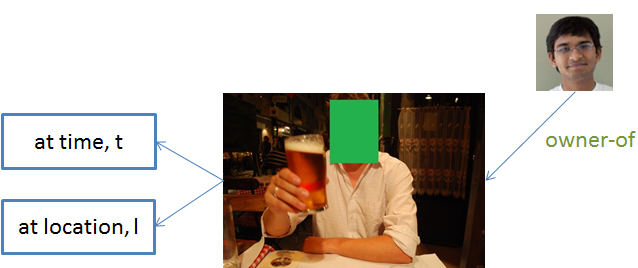
\includegraphics[width=0.75\textwidth]{media/chapter4/stacktrace/init-network.png}
\caption{Context Network built after User Information and EXIF sources are queried and merged.}
\label{fig:exif-network}
\end{figure}

Now, the algorithm traverses the graph to list all the possible queries it can execute on the data integration layer. Given the knowledge that entities participate in events, and events can contain participants, it generates the following queries:

\begin{itemize}
\item Does any data source contain participant information related to the photo capture event?
\item What events is the owner (entity:ArjunSatish) participating at time, t and location, l?
\end{itemize}

The data integration system looks at the different sources and says that none of them store information about photo capture events, and skips executing the first query. But many sources describe events, and store their participants too (Google Calendar, Facebook, Conference Calendar). These query is converted to their native formats (API calls or relational database queries) and results, are sent back to the data integration module. We see that there was a calendar entry returned be the Google Calendar source, as shown in \ref{fig:stacktrace-simple-calendar}. This information is now merged with the existing context graph to produce a context graph similar to that shown in \ref{fig:stacktrace-simple-context-network}.

\begin{figure}[h]
\centering
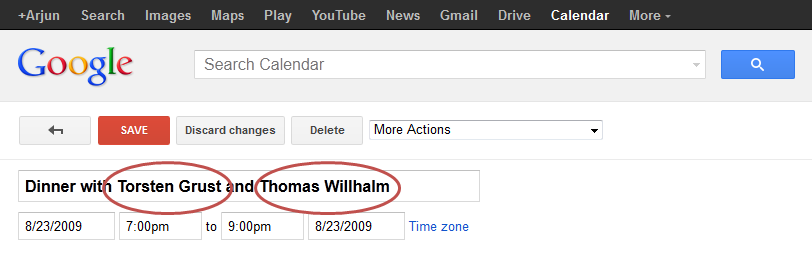
\includegraphics[width=\textwidth]{media/chapter4/stacktrace/calendar.png}
\caption{Calendar Event.}
\label{fig:stacktrace-simple-calendar}
\end{figure}

\begin{figure}[h]
\centering
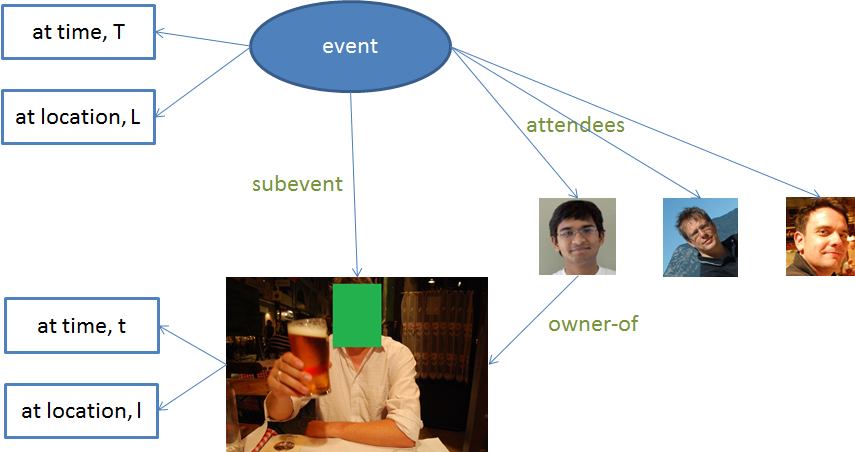
\includegraphics[width=0.75\textwidth]{media/chapter4/stacktrace/context-network-torsten.png}
\caption{Context Network after integrating calendar information.}
\label{fig:stacktrace-simple-context-network}
\end{figure}

Now, we have new entities related to the photo. The face verification algorithm is invoked with the new set of candidates. It must be noted that this verification problem is much easier than trying to verify out of many thousands of candidates. Once the correct entity is identified, the photo is annotated as shown in figure \ref{fig:stacktrace-simple-torsten-tagged}.

\begin{figure}[h]
\centering
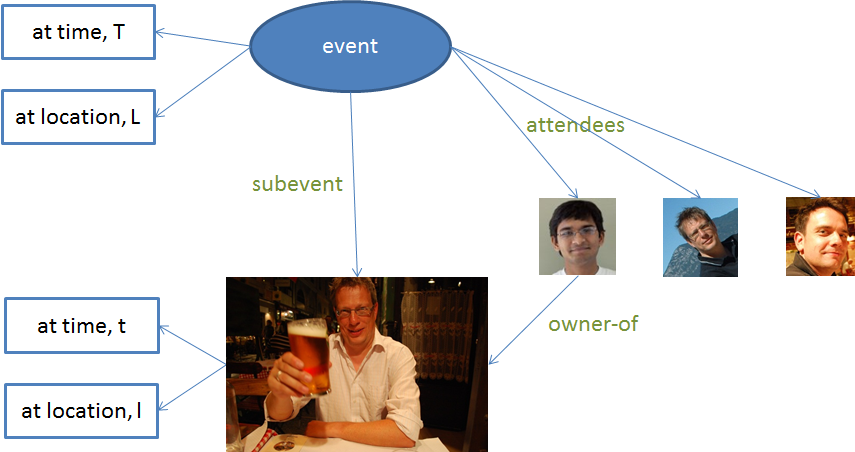
\includegraphics[width=0.9\textwidth]{media/chapter4/stacktrace/torsten-tagged.png}
\caption{The Conceptual Architecture of CueNet.}
\label{fig:stacktrace-simple-torsten-tagged}
\end{figure}

One last look at the source diagram in figure \ref{fig:stacktrace-simple-all} shows which data sources revealed interesting information related to this photo. In this case, EXIF provided some relevant context on when and where the photo was taken. The owner's personal calendar provided information on what event was occurring during the time of photo capture, and who else was involved in it.

\begin{figure}[h]
\centering

\includegraphics[width=0.75\textwidth]{media/chapter4/stacktrace/time-space-calendar-selected.png}
\caption{Sources which provided relevant context are highlighted by green circles.}
\label{fig:stacktrace-simple-all}
\end{figure}

\subsection{Complex Case}
Now, we will consider a more complex case which requires more than just metadata and personal sources for successful tagging. The photo under consideration is shown in \ref{fig:vldb-hidden}. We will use the same set of data sources, shown again in \ref{fig:vldb-sources}.

\begin{figure}[ht]
\begin{minipage}[b]{0.45\linewidth}
\centering
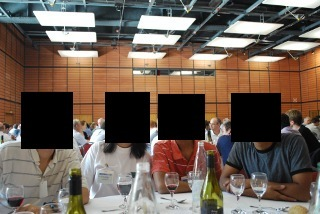
\includegraphics[width=\textwidth]{media/chapter4/stacktrace/vldb-hide-all.jpg}
\caption{Input Photo.}
\label{fig:vldb-hidden}
\end{minipage}
\hspace{0.5cm}
\begin{minipage}[b]{0.45\linewidth}
\centering

\includegraphics[width=\textwidth]{media/chapter4/stacktrace/sources.png}
\caption{Available Data Sources.}
\label{fig:vldb-sources}
\end{minipage}
\end{figure}

\begin{figure}[h]
\centering
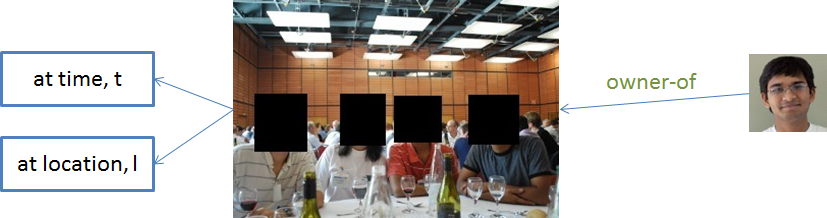
\includegraphics[width=0.9\textwidth]{media/chapter4/stacktrace/vldb-network-1.png}
\caption{Context Network built after User Information and EXIF sources are queried and merged.}
\label{fig:vldb-exif-network}
\end{figure}

Using metadata sources and personal information, we arrive at the context network shown in figure \ref{fig:vldb-exif-network}. The procedure until here is exactly same as that for the previous scenario. Now, given the known state of the world, if we invoke the face verification tools, we discover that the owner is actually present in the photo (figure \ref{fig:vldb-network-2}). In this case, the candidate set contains just one entity, and therefore reduces the complexity of the tagging algorithm.

\begin{figure}[h]
\centering
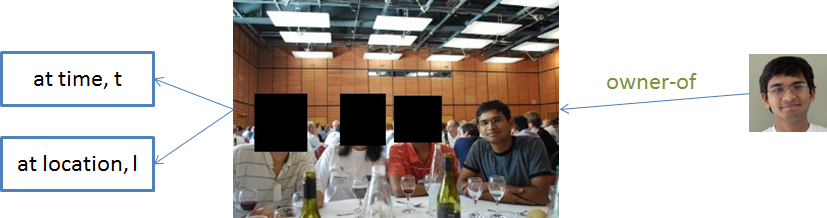
\includegraphics[width=0.9\textwidth]{media/chapter4/stacktrace/vldb-network-2.png}
\caption{Context Network built after User Information and EXIF sources are queried and merged.}
\label{fig:vldb-network-2}
\end{figure}

The next query generated by the system is to discover what the (entity:ArjunSatish) was doing at this time? But, this time we find that the conference calendar holds the answer.

\begin{figure}[h]
\centering
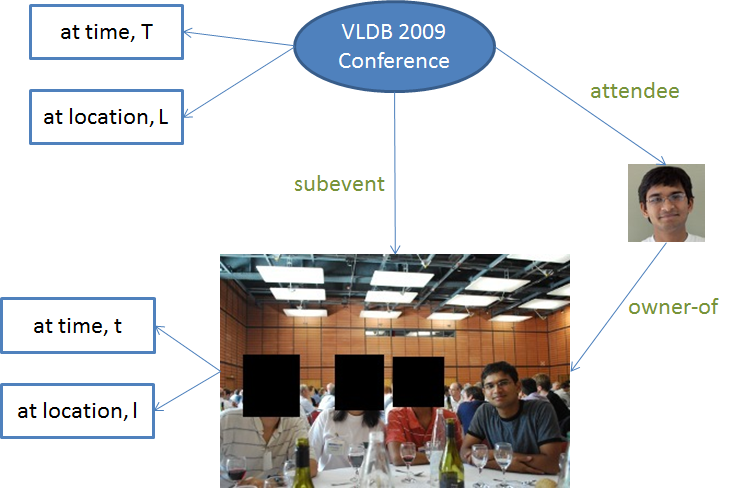
\includegraphics[width=0.75\textwidth]{media/chapter4/stacktrace/vldb-network-3.png}
\end{figure}
\begin{figure}[h]
\centering

\includegraphics[width=0.9\textwidth]{media/chapter4/stacktrace/vldb-source-1.png}
\caption{Context Network after querying conference sources.}
\label{fig:vldb-network-3}
\end{figure}

At this point, the conference event is known to our knowledge base to have a definite structure, in terms of keynote, session and talk events with lunch/coffee breaks interleaved, and having many attendees. So it immediately queries the conference source to find and merge all of these objects. It discovers that the photo was taken during a break event, and that the conference (VLDB 2009) has many hundreds of participants, as shown in figure \ref{fig:vldb-network-4}.

\begin{figure}[h]
\begin{minipage}[b]{0.5\linewidth}
\centering
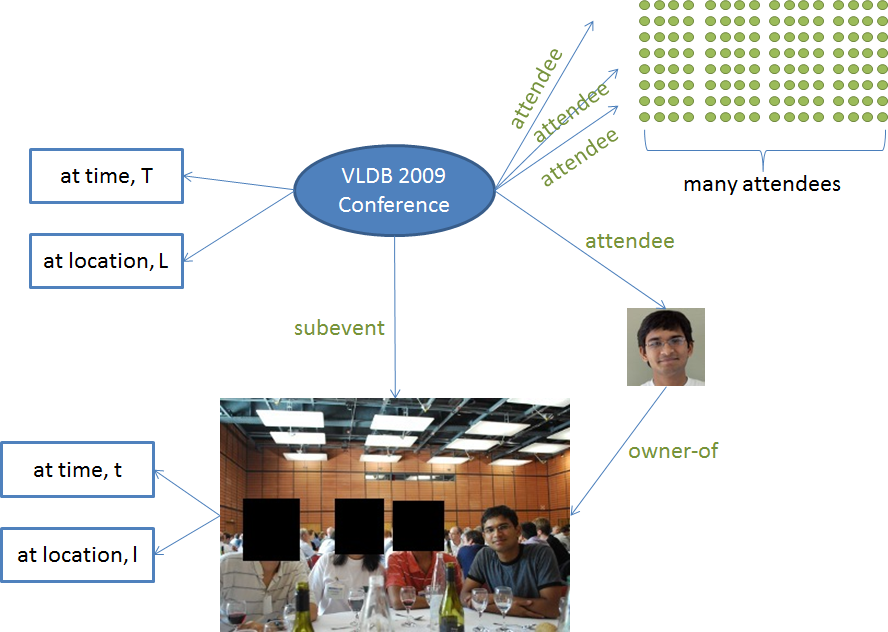
\includegraphics[width=\textwidth]{media/chapter4/stacktrace/vldb-network-4.png}
\caption{Context Network after discovering conference attendees.}
\label{fig:vldb-network-4}
\end{minipage}
\hspace{0.5cm}
\begin{minipage}[b]{0.5\linewidth}
\centering
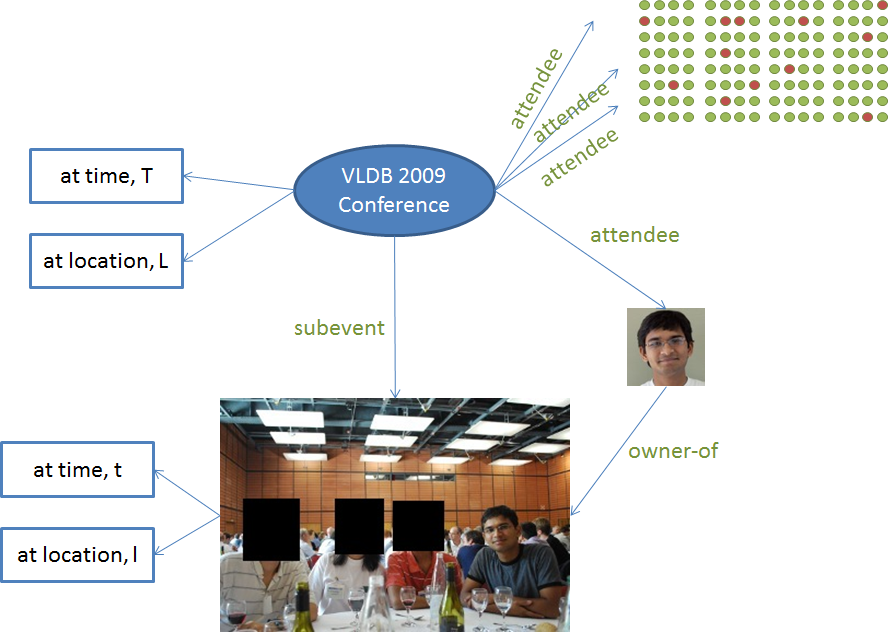
\includegraphics[width=\textwidth]{media/chapter4/stacktrace/vldb-network-5.png}
\caption{Context Network after discovering relations between attendees and owner.}
\label{fig:vldb-network-5}
\end{minipage}
\end{figure}

Figure \ref{fig:vldb-network-4} shows the various attendees discovered by the algorithm from the conference source. But finding 3 candidates from hundreds is an equally challening task. Before invoking the face tagging algorithm, we want to see if we can discover any more relations between the objects in the context network. So the discovery algorithm consults the knowledge base to find that entities can be related through a \textbf{friend-of} relation. So it queries all known sources to find friend relations, and finds that Facebook, Gmail and Twitter are sources which store data containing this relation. Querying it reveals that a few of the entities who were present at the conference were related to the user, and therefore have a bigger chance of appearing in the photo. The face verifier is invoked only with these candidates, for potential true positives. By doing this we tag two more faces in the photo. The context network is shown in the figure \ref{fig:vldb-network-6}.

\begin{figure}[h]
\centering
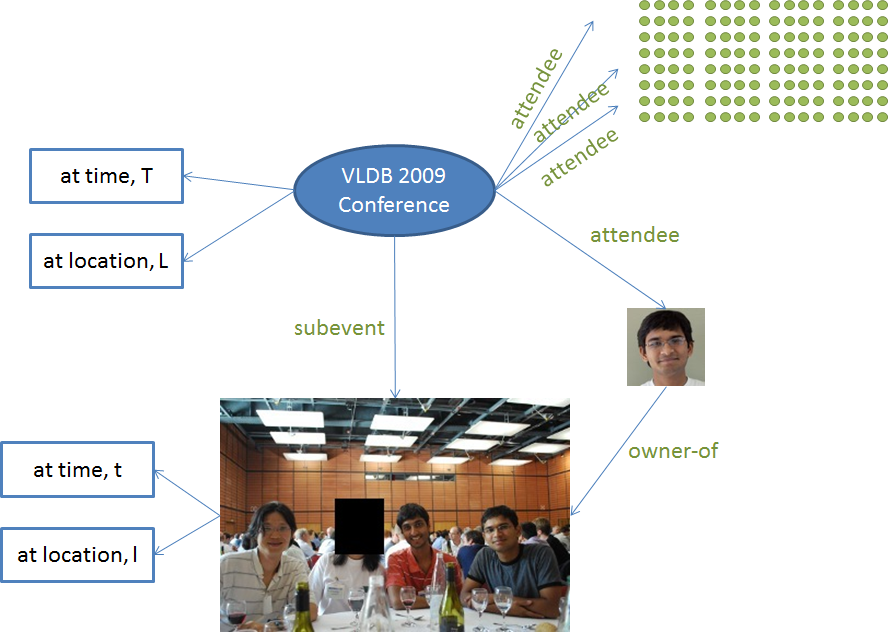
\includegraphics[width=0.75\textwidth]{media/chapter4/stacktrace/vldb-network-6.png}
\caption{Context Network after discovering social relations.}
\label{fig:vldb-network-6}
\end{figure}
\begin{figure}[h]
\centering

\includegraphics[width=0.9\textwidth]{media/chapter4/stacktrace/vldb-source-2.png}
\caption{Sources used so far.}
\label{fig:vldb-network-3}
\end{figure}

Since we have more candidates tagged in the photo, we can repeat the above procedure to discover more relation between the entites related to the photo and those who are present in the conference. This time results are returned from Gmail, and none from Facebook and Twitter (because these people had sent emails to each other during the conference, but did not connect through Facebook or Twitter). The changes in the context network are shown in \ref{fig:vldb-network-7} and \ref{fig:vldb-network-8}. Figure \ref{fig:vldb-network-3} highlights all sources which returned relevant context for this trace. 

\begin{figure}[h]
\begin{minipage}[b]{0.5\linewidth}
\centering
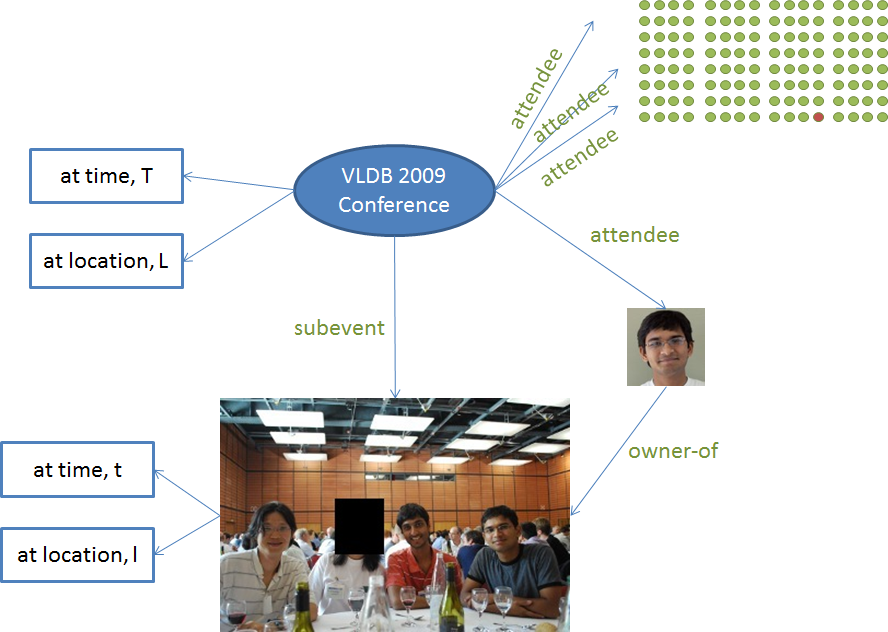
\includegraphics[width=\textwidth]{media/chapter4/stacktrace/vldb-network-7.png}
\caption{Context Network after discovering further social relations.}
\label{fig:vldb-network-7}
\end{minipage}
\hspace{0.5cm}
\begin{minipage}[b]{0.5\linewidth}
\centering
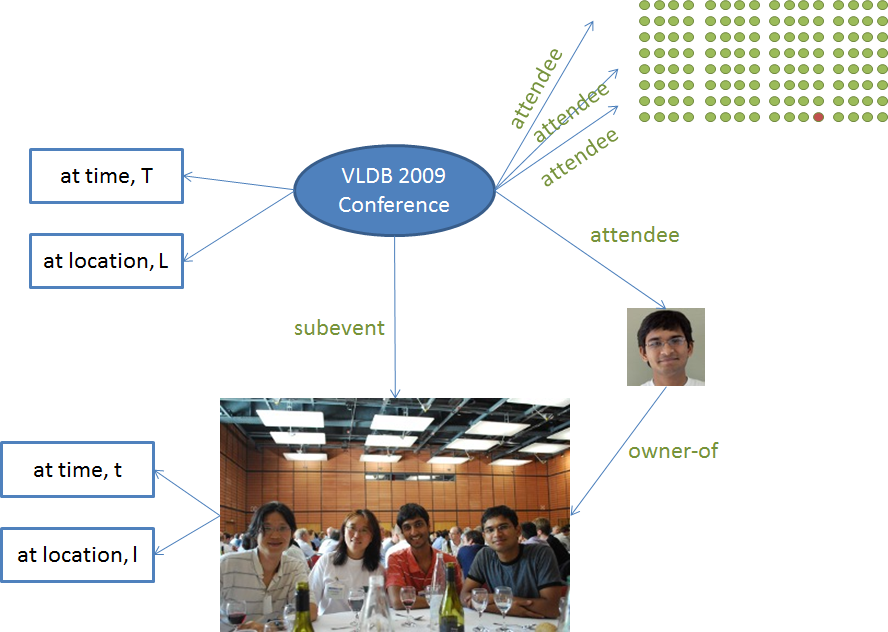
\includegraphics[width=\textwidth]{media/chapter4/stacktrace/vldb-network-8.png}
\caption{Context Network after tagging all faces.}
\label{fig:vldb-network-8}
\end{minipage}
\end{figure}

\begin{figure}[h]
\centering

\includegraphics[width=\textwidth]{media/chapter4/stacktrace/vldb-source-3.png}
\caption{Sources used to tag all faces.}
\label{fig:vldb-network-3}
\end{figure}


\section{Event Model}
Our ontologies extend the E* model\cite{gupta2011managing} to specify relationships between events and entities. Specifically, we utilize the relationships ``\textbf{subevent-of}", which specifies event containment. An event $e1$ is a subevent-of of another event $e2$, if $e1$ occurs completely within the spatiotemporal bounds of $e2$. Additionally, we utilize the relations \textbf{occurs-during} and \textbf{occurs-at}, which specify the space and time properties of an event. Also, another important relation between entities and events is the ``\textbf{participant}" property, which allows us to describe which entity is participating in which event. It must be noted that participants of a subevent are also participants of the parent event. A participation relationship between an event and person instance asserts the presence of the person within the spatiotemporal region of the event. We argue that the reverse is also true, i.e., if a participant $P$ is present in $\mathcal{L}_P$ during the time $\mathcal{T}_P$ and an event $E$ occurs within the spatiotemporal region $<\mathcal{L}_E$, $\mathcal{T}_E>$, we say $P$ is a participant of $E$ if the event's spatiotemporal span contained that of the participant.
\begin{equation}
\label{eq:participation-region}
\begin{aligned}
\text{\texttt{participant}(E, P)} \iff (\mathcal{L}_P \sqsubset_L \mathcal{L}_E) \wedge (\mathcal{T}_P \sqsubset_T \mathcal{T}_E)
\end{aligned}
\end{equation}
The symbols $\sqsubset_L$ and $\sqsubset_T$ indicate spatial and temporal containment respectively. Please refer to \cite{gupta2011managing} for more details. In later sections, we refer to the location and time of the event, $\mathcal{L}_E$ and $\mathcal{T}_E$ as $E$.\textbf{occurs-at} and $E.$\textbf{occurs-during} respectively. 

\begin{figure*}[t]
\centering
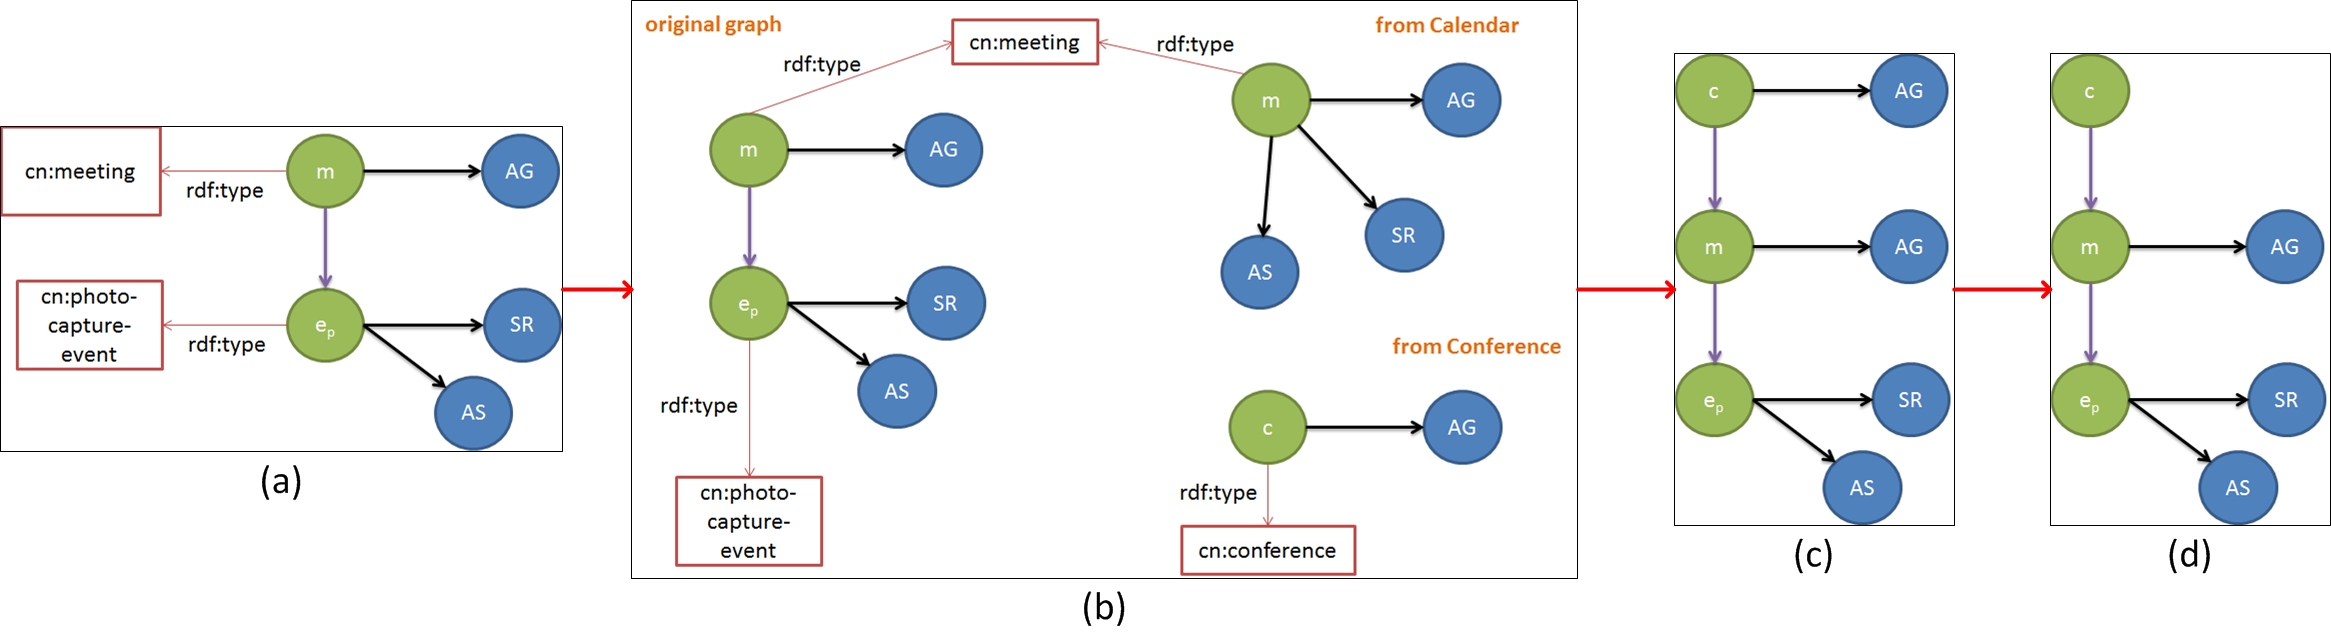
\includegraphics[width=\textwidth]{media/exec/exec-cycle-one-line.png}
\caption{The various stages in an iteration of algorithm \ref{alg:cx-alg}.}
\label{fig:exec-cycle}
\end{figure*}

\section{Data Sources}
\label{sec:data-sources}
The ontology makes available a vocabulary of classes and properties. Using this vocabulary, we can now declaratively specify the schema of each source. With these schema descriptions, CueNet can infer what data source can provide what type of data instances. For example, the framework can distinguish between a source which describes conferences and another which is a social network. We use a LISP like syntax to allow developers of the system to specify these declarations. The example below describes a source containing conference information.

\begin{verbatim}
(:source conferences
   (:attrs url name time location title)
   (:rel conf type-of conference)
   (:rel time type-of time-interval)
   (:rel loc type-of location)
   (:rel attendee type-of person)
   (:rel attendee participant-in conf)
   (:rel conf occurs-at loc)
   (:rel conf occurs-during time)
   (:axioms
      (:map time time)
      (:map loc location)
      (:map conf.title ltitle)
      (:map conf.url url)
      (:map attendee.name name)))
\end{verbatim}

% The above source declaration consists of a s-expression, where the source keyword indicates a unique name for the source. The \texttt{attrs} keyword is used to list the attributes of this source. The \texttt{rel} keyword constructs the instances conf, time, loc, attendee which are of conference, time-interval, location and person class types respectively, and relates them with relations specified in the ontology. Finally, the mapping \texttt{axioms} are used to map nodes in the relationship graph constructed above to attributes of the data source. For example, the first axiom (specified using the map keyword) maps the time node to the time attribute. 

A source declaration comprises of a single nested s-expression. We will refer to the first symbol in each expression as a keyword, and the following symbols as operands. This above declaration uses five keywords (\texttt{source}, \texttt{attrs}, \texttt{rel}, \texttt{axioms}, \texttt{map}).  The \texttt{source} keyword is the root operator, and declares a unique name of the data source. The source mapper can be queried for finding accessors using this name. The \texttt{attrs} keyword is used to list the attributes of this source. Currently we assume a tuple based representation, and each operand in the attrs expression maps to an element in the tuple. The \texttt{rel} keyword allows construction of a relationship graph where the nodes are instances of ontology concepts. And edges are the relationships described by this particular source. In the above example, we construct individuals \textit{conf}, \textit{time}, \textit{loc} and \textit{attendee} who are instances of the \textit{conference}, \textbf{time-interval}, \textbf{location} and \textbf{person} class respectively. We further say that attendee is a \textbf{\textit{participant of}} the conference, which \textbf{\textit{occurs-at}} location loc and \textbf{\textit{occurs-during}} the interval time. Finally, the \texttt{mapping axioms} are used to map nodes in the relationship graph to attributes of the data source. For example, the first axiom (specified using the map keyword) maps the time node to the time attribute. The third map expression creates a literal called title, and associates it to the conference node, whose value comes from the ltitle attribute of the conference data source.

Formally, we represent the given ontology as $O$. The various classes and properties in $O$ are represented by $C^O$ and $P^O$ respectively. Since our upper ontology consists of DOLCE and E*, we assume the inclusion of the classes \texttt{Endurant}, \texttt{Perdurant}, \texttt{Event} and \texttt{Person} in $C^O$. Each source $S$ consists of three parts, a relation graph $G^S(V^S, E^S)$ where the nodes $V^S \in C^O$, specify the various ``things'' described by the source. The edges $E^S \in P^O$ specify the relations among the nodes. Any graph retrieved from such a source is an instance of the relation graph, $G^S$. Further, the tuple $A^S_T$ consists of the attributes of the data source. Finally, the mapping $M^S: \{G^S \rightarrow A^S_T\}$ specifies how to map different nodes in the relation graph to the different attributes of the native data source.

\section{Conditions for Discovery}
CueNet is entirely based on reasoning in the event and entity (i.e., person) domain, and the relationships between them. These relationships include participation (event-entity relation), social relations (entity-entity relation) and subevent relation (event-event). For the sake of simplicity, we restrict our discussions to events whose spatiotemporal spans either completely overlap or do not intersect at all. We do not consider events which partially overlap. In order to develop the necessary conditions for context discovery, we consider the following two axioms:

\textbf{Entity Existence Axiom}: Entities can be present in one place at a time only. The entity cannot exist outside a spatiotemporal boundary containing it.

\textbf{Participation Semantics Axiom}: If an entity is participating in two events at the same time, then one is the subevent of the other. 

% Before we provide an overview of the discovery algorithm, we must make a note of set of conditions required for its correct execution. 

Given, the ontology $O$, we can construct event instance graph $G^I(V^I, E^I)$, whose nodes are instances of classes in $C^O$ and edges are instances of the properties in $P^O$. The context discovery algorithm relies on the notion that given an instance graph, \textit{queries} to the different sources can be automatically constructed. A query is a set of predicates, with one or more unknown variables. For the instance graph $G^I (V^I, E^I)$, we construct a query $Q(D, U)$ where $D$ is a set of predicates, and $U$ is a set of unknown variables.

\textbf{Query Construction Condition:} Given an instance graph $G^I (V^I, E^I)$ and ontology $O(C^O, P^O)$, a query $Q(D, U)$ can be constructed, such that $D$ is a set of predicates which represent a subset of relationships specified in $G^I$. In other words, $D$ is a subgraph induced by $G^I$. $U$ is a class, which has a relationship $r \in P^O$, with a node $n \in D$. Essentially, the ontology must prescribe a relation between some node $n$ through the relationship $r$. In our case, the relation $r$ will be either a \textbf{participant} or \textbf{subevent} relation. If the relationship with the instances does not violate any object property assertions specified in the ontology, we can create the query $Q(D, U)$.

\textbf{Identity Condition:} Given an instance graph $G^I(V^I, E^I)$, and a result graph $G^R(V^R, E^R)$ obtained from querying a source, we can merge two events only if they are identical. Two nodes $v^I_i \in V^I$ and $v^R_r \in V^R$ are identical if they meet the following two conditions \textbf{(i)} Both $v^I_i$ and $v^R_r$ are of the same class type, and \textbf{(ii)} Both $v^I_i$ and $v^R_r$ have exactly overlapping spatiotemporal spans, indicated by the $=_L$ and $=_T$. Mathematically, we write: 
\begin{equation}
\label{eq:identity}
\begin{aligned}
v^I_i = v^R_r \iff (v^I_i.\text{\textbf{type-of}} = v^R_r.\text{\textbf{type-of}}) \wedge \\ 
(v^I_i.\text{\textbf{occurs-at}} =_L v^R_r.\text{\textbf{occurs-at}}) \wedge \\
(v^I_i.\text{\textbf{occurs-during}} =_T v^R_r.\text{\textbf{occurs-during}})
\end{aligned}
\end{equation}
\textbf{Subevent Condition:} Given an instance graph $G^I(V^I, E^I)$, and a result graph $G^R(V^R, E^R)$ obtained from querying a source, we can construct a subevent edge between two nodes $v^I_i \in V^I$ and $v^R_r \in V^R$, if one is spatiotemporally contained within the other, and has at least one common \texttt{Endurant}.
\begin{equation}
\label{eq:sube-st-containment}
\begin{aligned}
   v^I_i \sqsubset_L v^R_r,\\
   v^I_i \sqsubset_T v^R_r
\end{aligned}
\end{equation}
\begin{equation}
\label{eq:sube-entity-containment}
\begin{aligned}
   v^I_i.\text{\textbf{Endurants}} \cap v^R_r.\text{\textbf{Endurants}} \neq \{\phi\}\\
\end{aligned}
\end{equation}
Here $v^I_i.$\textbf{Endurants} is defined as a set $\{w | w \in V^I_i \wedge w.$type-of$ = $Endurant$\}$. If equation \eqref{eq:sube-entity-containment} does not hold, we say that $v^I_i$ and $v^R_r$ co-occur.

\textbf{Merging Event Graphs}: Given the above conditions, we can now describe an important building block for the context discovery algorithm: the steps needed to merge two event graphs. An example for this is shown in figure \ref{fig:exec-cycle}(b-d). Given the event graph consisting of the photo capture event on the left of (b) and a meeting event $m$ and conference event $c$, containing their respective participants. In this example, the meeting event graph, $m$ is semantically equivalent to the original graph. But the conference event, $c$ is telling that the person $AG$ is also participating in a conference at the time the photo was taken. The result of merging is shown in (d). An event graph merge consists of two steps. The first is a \texttt{subevent hierarchy join}, and the second is a \texttt{prune-up} step. 

Given an original graph, $O_m$, and a new graph $N_m$, the join function works as follows: All nodes in $N_m$ are checked against all nodes in $O_m$ to find identical counterparts. For entities, the identity is verified through an identifier, and for events, equation \eqref{eq:identity} is used. Because of the entity existence and participation semantics axioms, all events which contain a common participant are connected to their respective super event using the subevent relation (equations \eqref{eq:sube-st-containment} and \eqref{eq:sube-entity-containment} must be satisfied by the events). Also, if two events have no common participant, then they can be still be related with the subevent edge, if the event model says it is possible. For example, if in a conference event model, keynotes, lunches and banquets are declared as known subevents of an event. Then every keynote event, or banquet event to be merged into an event graph is made a subevent of the conference event, if the equation \eqref{eq:sube-st-containment} holds between the respective events. 

It must be noted that node $AG$ occurs twice in graph (c). In order to correct this, we use the participation semantics axiom. We traverse the final event graph from the leaves to the root events, and remove every person node if it appears in a subevent. This is the \texttt{prune-up} step. Using these formalisms, we now look at the working of the context discovery algorithm. 

\restylealgo{ruled}
\SetAlgoSkip{}
\begin{algorithm}[h]
\dontprintsemicolon 
\KwData{A photograph H, with a set of detected faces F. Voting threshold, T. The owner O of the photo.}
\KwResult{For each face f $\in$ F, a set of atmost $k$ person tags.}
\Begin{
  
  $ $\;
  function discover(): \{ \;
  \Indp while (\texttt{DQ} is not empty): \{ \;
  \Indp \texttt{node} = \texttt{DQ}.deque() \;
  \texttt{results} = query (\texttt{node}) \;
  \texttt{E} $\leftarrow$ merge (\texttt{E}, \texttt{results}) \;
  if (termination\_check()): \;
  \Indp \textbf{return} prepare\_results(); \;
  \Indm
  \Indm
  \} \;
  reconstruct \texttt{DQ} $\leftarrow$ \texttt{E} \;
  discover() \;
  \Indm
  \}\;
  
  $ $\;
  
  function merge(\texttt{O}, \texttt{N}): \{ \;
    \Indp 
    remove\_duplicates() \;
    \texttt{M} $\leftarrow$ subevent\_hierarchy\_join(\texttt{O}, \texttt{N}) \;
    prune\_up(\texttt{M}) \;
    if (less than \texttt{T} new candidates were discovered): \; {
    \Indp
  	    push\_down(\texttt{M}) \;
  	\Indm
    } else: \; 
    \Indp
	    vote\_and\_verify(\texttt{M}) \;
  	\Indm
 	return \texttt{M}; \;
  \Indm
  \} 
  
  $ $ \;
  \texttt{E} $\leftarrow$ construct event graph with \texttt{H} and \texttt{O} \;
  construct discoverable nodes queue, \texttt{DQ} $\leftarrow$ \texttt{E} \;
  \textbf{return} discover() \;
  
}
\caption{The Context Discovery Algorithm}
\label{alg:cx-alg}
\end{algorithm}

\subsection{Context Discovery Algorithm}
\label{sec:discovery-algorithm}
Algorithm \ref{alg:cx-alg} below outlines the tail recursive discovery algorithm. The input to the algorithm is a photo (with EXIF tags) and an associated owner (the user). It must be noted that by seeding the graph with owner information, we bias the discovery towards his/her personal information. An event instance graph is created where each photo is modeled as a photo capture event. Each event and entity is a node in the instance graph. Each event is associated with time and space attributes. All relationships are edges in this graph. All EXIF tags are literals, related to the photo with data property edges. Figure \ref{fig:exec-cycle} graphically shows the main stages in a single iteration of the algorithm.

The event graph is traversed to produce a queue of entity and event nodes, which we shall refer to as DQ (discovery queue). The algorithm consists of two primary functions: \textbf{discover} and \textbf{merge}. The discover function is tail recursive, invoking itself until a termination condition is reached (when at most $k$ tags are obtained for all faces or no new data is obtained from all data sources for all generated queries). The behavior of the query function depends on the type of the node. If the node is an event instance, the function consults the ontology to find any known sub-events, and queries data sources to find all these subevents, its properties and participants of the input event node. On the other hand, if it is an entity instance, the function issues a query to find all the events it is participating in. 

Results from data source wrappers are returned in the form of event graphs. These event graphs are merged into the original event graph by taking the following steps. First, it identifies \textbf{duplicate} events using the conditions mentioned above. Second, it identifies subevent hierarchies using the graph merge conditions described above, and performs a \textbf{subevent hierarchy join}. Third, the function \textbf{prune-up} removes entities from an event when its subevent also lists it as a participant node. Fourth, \textbf{push-down} is the face verification step if the number of entities in the parents of the photo-capture events is small (less than $T$). Push down will try to verify if any of the newly discovered entities are present in the photo and if they are (if the tagging confidence is higher than the given threshold), the entities are removed from the super event, and linked to the photo capture event as its participant. On the other hand, if this number is larger than T, the algorithm initiates the \textbf{vote-and-verify} method, which ranks all the candidates based on social relationships with people already identified in the photo. For example, if a candidate is related to two persons present in the photo through some social networks, then its score is 2. Ranking is done by simply sorting the candidate list by descending order of score. The face verification runs only on the top ranked $T$ candidates. If there are still untagged faces after the termination of the algorithm, we vote over all the remaining people, and return the ranked list for each untagged face.

Figure \ref{fig:exec-cycle} shows the various stages in the algorithm graphically. (a) shows an example event graph describing a photo taken at a meeting. The meeting consists of three participants AG, SR and AS. The photo contains SR and AS. (b) shows two events returned from the data sources. One is a meeting event which is semantically identical to the input. The other is a conference event with AG. (c) shows the result of merging these graphs. (d) The \texttt{prune-up} function removes the duplicate reference to AG. \underline{A live visualization of these steps for different photos can be found at \href{http://cuenet.site44.com/}{http://cuenet.site44.com}}.

\section{Implementation}

\chapter{Experiments and Analysis}

In this chapter, we will present experiments to show the efficacy of the context discovery approach. Experiments will be performed on real-world data from real users using a variety of social and personal media applications, public data sources. The motivation behind these experiments is to tag faces in thousands of personal photos taken by various people at a different events. We will also perform experiments on generated data to simulate large scale use cases. Here, the motivation is to analyze the performance characteristics of the merge algorithm.

\section{Experiments on Real-World Data}
In this section, we analyze how CueNet helps tags a person's photos taken at different types of events. For a given users, we will construct a dataset consisting of photos taken at a particular event. For each of these users, we will create a candidate set by aggregating people over personal, public and social data sources. In order to evaluate CueNet, we will attempt to reduce this candidate set, and analyze how many of the faces can be correctly tagged by this reduced set. We will also compare this performance over metrics like location based ranking, where candidates are ranked according to their last known location, and (if time permits) tie strength. Our final conclusion is that, in order to rank candidates for tagging faces in photos, CueNet provides an event-agnostic platform, where as other techniques perform inconsistently across different types of events.

\subsection{Setup}
We use photos taken during three different \textbf{types of events}: Social Parties, Academic Conferences and Trips. This diversity allows for different distributions of face tags across different aspects of a user's life. Social Parties generally tend to have close friends who are spatially co-located. Conferences tend to have people from different parts of the world, but those who are affiliated with the area of the conferences. Trips, cannot always rely on location as a useful metric and can involve people from either social, personal or professional circles from a user's life. 

For each event type, we collect multiple datasets from 6 different people. A \textbf{dataset} consists of multiple photos during the event, the user's personal information, which contains information from sources like Google Calendar, personal email and profile information from social networks like Facebook and Twitter. We also collect a person's social networking information which consists of tweets written by the user or their friend during the time the event was occurring, the social network itself (friends on Facebook and Twitter, along with their profile information). Conference proceedings are downloaded from DBLP and the conference website. Facebook events are also obtained and stored in our database. Besides, location databases like Yahoo Placefinder were used to geocode addresses and reverse geocode EXIF GPS coordinates. We assume that all photos have a valid EXIF tag, especially the timestamp and GPS coordinates. This assumption is not a very hard one, as almost all photos captured in the last two years are through iPhone or Android smartphones, which add reasonably accurate GPS tags and accurate timestamps (where the phone clock is synced with the cell tower). The domination of iPhone in the photo market is shown in figure \ref{fig:flickr-camera-popularity}. The ground truth was annotated by the user with our annotation interface. For each photo, an annotation consisted of the ID of the person in the candidate set in it. Face verification was achieved initially with Face.com, but after their website was shutdown, we used the web service, Automatic Face Systems, maintained by Neeraj Kumar. After this service was terminated, we resorted to manual face verification. We use the manual verification for the experiments described below, unless otherwise mentioned.

\begin{figure}[t]
\centering
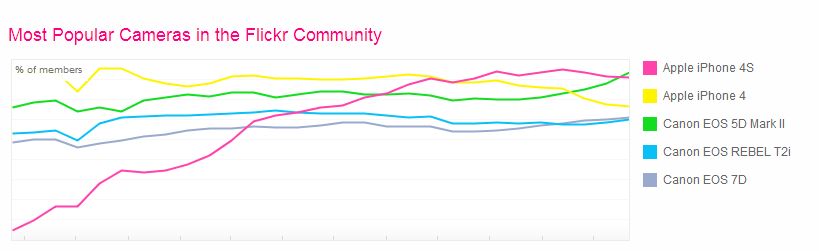
\includegraphics[width=0.9\textwidth]{media/flickr-camera-popularity.png}
\caption{Popularity of iPhone at Flickr.com (October 2011).}
\label{fig:flickr-camera-popularity}
\end{figure}

In order to construct a \textbf{candidate set} for each dataset, we construct a so-called \texttt{CandidateSet}. A \texttt{CandidateSet} data structure performs two functions. It is a persistent set of candidates each of which have a unique identifier. Second, each data source, which has its own identifier for a candidate can look up the candidate set with this identifier to obtain the candidate set identifier. Here is an example of a simple candidate set:

\begin{verbatim}
[
{csid: 1010-poqs, name: `Arjun Satish', email: `arjun@uci.edu', 
                                        email: `arjun.satish@gmail.com',
                                        facebook-id: `656563332'}
{csid: 2010-pasd, name: `Ramesh Jain', email: `jain@ics.uci.ed',
                                       name: `Dad',
                                       email: `jain49@gmail.com',
                                       facebook-id: `10004290384'}
{csid: 1255-juen, name: `Peter Boncz', confid: `cf-12-candidate-322'}
{csid: 7585-kdye, name: `Amarnath Gupta', email: `gupta@sdsc.edu',
                                          twitter: `aguptasd'}
{csid: 1111-bmel, name: `Arjun', twitter: `@wicknicks'}
]
\end{verbatim}

The above snippet is a part of the candidate set created during the tagging of my personal photos. A \texttt{CandidateSet} is a multimap where the keys are the unique IDs (shown as csid above). The values are a list of key-value attribute pairs. The key could be a global key, such as name or email address, which can be added by any data source. In the above example, different sources could contribute different names for the same entity. Same values for the same key are not duplicated. The list could contain keys which are local to a data source, for example the facebook identifier key: \texttt{facebook-id}. This primarily helps in querying the candidate set to obtain a reference to the candidate during the discovery phase. 

The construction of the \texttt{CandidateSet} happens when the system is brought up. For each user, a unique \texttt{CandidateSet} is created, or loaded if it exists on disk. In order to create it, each data source is probed individually to provide a list of unique persons. The data source mediator checks if the user already exists in the \texttt{CandidateSet} through its local primary key, and if he does, adds additional key value pairs to the attribute list. If a candidate corresponding to its primary key does not exist, a new candidate is created in the set, and the local primary key is added as an attribute pair. This technique will fail to merge different identities of people if they use multiple email addresses or do not store email information on social networks. Thus, we create a merge file, which lists a set of merges between candidates. In the above example, we will use this functionality to combine the entries with IDs \texttt{1111-bmel} and \texttt{1010-poqs} into a unified candidate. This gurantees that context discovered for one online identity is propagated to other identities of the same person.

We use 1889 photos taken at 17 different events in our face tagging experiment. Each photo contains one or more faces. We will denote each dataset as `Di' (where 1 $\leq$ $i$ $\leq$ 17 for each dataset). Table \ref{tbl:unique-persons} describes each dataset in terms of number of photos, unique annotations in ground truth, the year they were captured and the type of the event. 

\begin{table}[h]
\begin{center}
\begin{tabular}{ |c|p{1.5cm}|p{1.5cm}|c|p{2.5cm}|c| }
  \hline
  \texttt{Dataset} & \texttt{Unique People} & \texttt{No.\ of Photos} & \texttt{Year} & \texttt{CandidateSet Size} & \texttt{Event Type}\\
  \hline
     D1  &  43   &   78   &  2012  &  660   & conference \\
     D2  &  24   &   108  &  2012  &  660   & conference \\
     D3  &  6    &   16   &  2010  &  660   & conference \\
     D4  &  7    &   10   &  2010  &  660   & conference \\
     D5  &  36   &   80   &  2009  &  660   & conference \\
     D6  &  18   &   65   &  2013  &  660   & conference \\
     D7  &  7    &   11   &  2013  &  660   & conference \\
     D8  &  12   &   25   &  2009  &  1894  & conference \\
     D9  &  14   &   65   &  2011  &  215   & party \\
    D10  &  13   &   131  &  2010  &  561   & party \\
    D11  &  6    &   85   &  2008  &  656   & party \\
    D12  &  50   &   74   &  2012  &  1049  & party \\
    D13  &  19   &   330  &  2009  &  691   & party \\
    D14  &  14   &   363  &  2009  &  711   & trip \\
    D15  &  2    &   208  &  2010  &  715  & trip \\
    D16  &  4    &   217  &  2011  &  711  & trip \\
    D17  &  7    &   23   &  2011  &  584  & trip \\
  \hline
\end{tabular}
\caption{Profile of datasets used in the experiments.}
\label{tbl:unique-persons}
\end{center}
\end{table}

We divide the sources into different categories to facilitate a more general discussion. The categories are ``Personal Information" (same as Owner Information in section \ref{sec:discovery-algorithm}), ``Event sources", and ``Social Networks". Event sources include Facebook events, Yahoo Upcoming web service, our conference events database among other sources. Social networks include Facebook's social graph. Personal information contained information about the user, and a link to their personal calendars. An annotation is considered ``Out of Context Network" if it is not in any of these sources.

\begin{figure}[t]
\centering
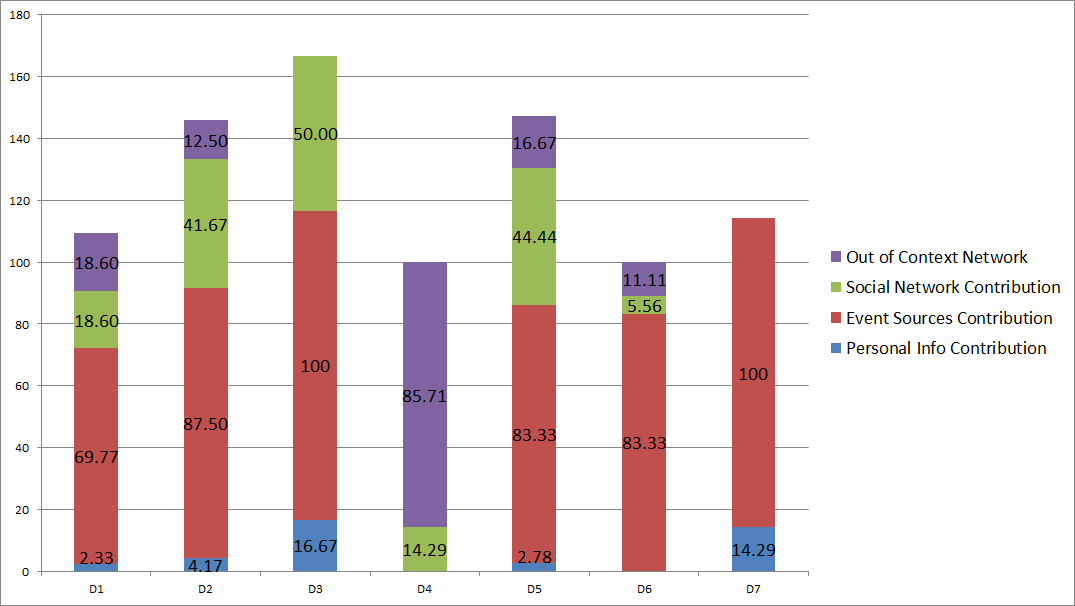
\includegraphics[width=0.9\textwidth]{media/gt-distro-stacked-2.png}
\caption{The distribution of annotations in the ground truth across various sources.}
\label{fig:src-cand-distribution}
\end{figure}

Figure \ref{fig:src-cand-distribution} shows the distribution of the ground truth annotations of the conference datasets across various sources, for each dataset. For example, the bar corresponding to D2 says that 87.5\% of ground truth annotations were found in event sources, 41.67\% in social networks, 4.17\% in personal information and 12.5\% were not found in any source, and therefore marked as ``Out of Context Network". From this graph it is clear that event sources contain a large portion of ground truth annotations. Besides D4, a minimum of 70\% of our annotations are found in event sources for all datasets, and for some datasets (D3, D7) all annotations are found in event sources. The sum total of contributions will add up to values more than 100\% because they share some annotations among each other. For example, a friend on Facebook might show up at a conference to give the keynote talk.

\subsection{Individual List Sizes in a Dataset}
First, we look at how CueNet reduces the number of possible candidates for all photos in a dataset. For this setup, the complete candidate set $L$, contained 1894 labels (total number of people present at the conference, user's emails and social graph). The figure \ref{fig:exp-vldb-all-cx} shows various statistics for each photo, which includes the maximum size of the list which was generated by the discovery algorithm, the actual number of people in the photos, the number of true positives and false positives. As it can be seen, the size of the discovered set $S$, never exceeded 12. This is 0.5\% of the original candidate list. Because the total number of possible participants (list size) was low, our False Positive rate (FP) was very low too. Most of the false positives were due to profile orientation of faces or obstructions (this was because the face detector was smart enough to pick up profile faces, but verification worked better only on frontal faces).

\begin{figure}[t]
\centering
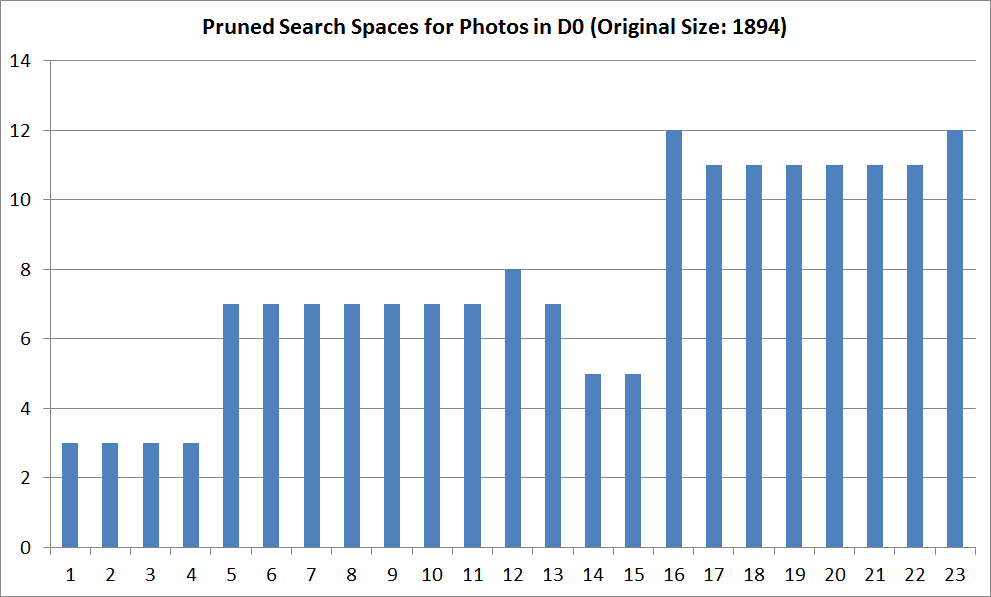
\includegraphics[width=0.9\textwidth]{media/reduced-list-sizes-d0.png}
\caption{Pruned search space for photos in conference dataset D8.}
\label{fig:exp-vldb-all-cx}
\end{figure}

\subsection{Results using Context Discovery}
In order to evaluate 17 different datasets, we perform the following modification on each dataset. For a dataset, we select the photo with all annotations, and attempt to tag it. The numbers seen below will reflect the results for such a photo. Alternatively, the numbers below can be interpreted as tagging the event itself, and not individual photos. We do this modification to reduce the number of graphs drawn per experiment. We define a \textbf{hit} as a correctly tagged face. Figure \ref{fig:exp-cx-hits} shows the hits for datasets using the context discovery algorithm. The blue bars show the number of unique faces in the dataset. As we can see the number of hits is equal to the number of unique faces, which implies that our context discovery algorithm was able to find the correct face tags for almost all datasets. Only for dataset 4, this difference is significant. This is because there was no contextual information related to the people in this dataset.

\begin{figure}[t]
\centering
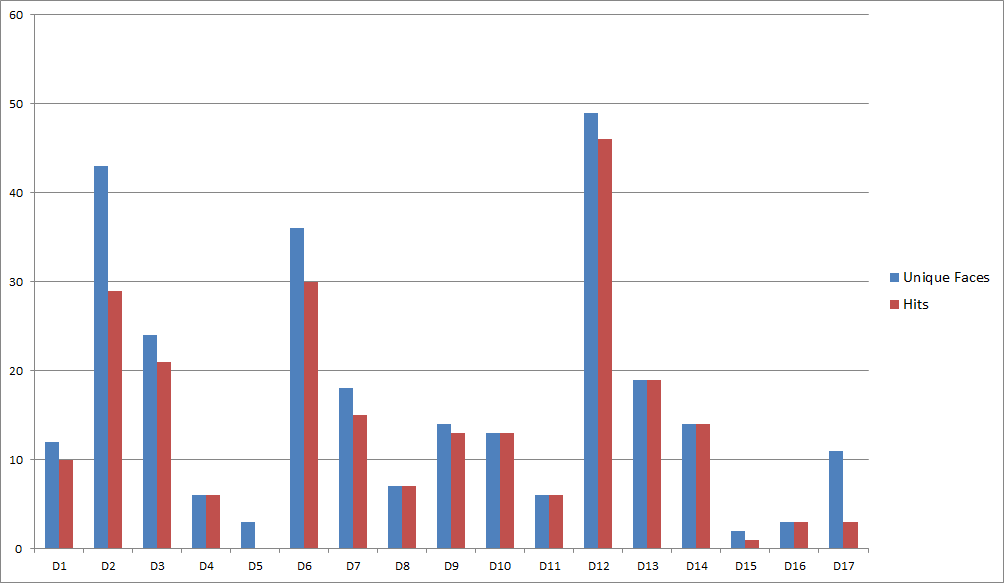
\includegraphics[width=0.9\textwidth]{media/chapter5/cx-unique-faces-hits-all-datasets.png}
\caption{Hit counts for all datasets using Context Discovery Algorithm.}
\label{fig:exp-cx-hits}
\end{figure}

Most of the datasets contain hundreds of candidates. If we have to perform face verification on all datasets, then the discovery algorithm is not performing effectively. The fewer the number of verifications, the better the accuracy of the algorithm. In order to quantify this, we introduce the metric \textit{Verification Ratio}, which is simply the number of verifications done per candidate in the \texttt{CandidateSet}. If this number is equal to 1, that means we have performed a very large number of verifications. The closer it is to 0, the fewer the number of verifications that were done. This ratio also enables us to compare the differences across dataset, where the number of candidates vary. As it can be seen in figure \ref{fig:exp-cx-verification-ratio}, the verification ratio never exceeds 19\% (the maximum value being 18.3\%).

\begin{figure}[t]
\centering
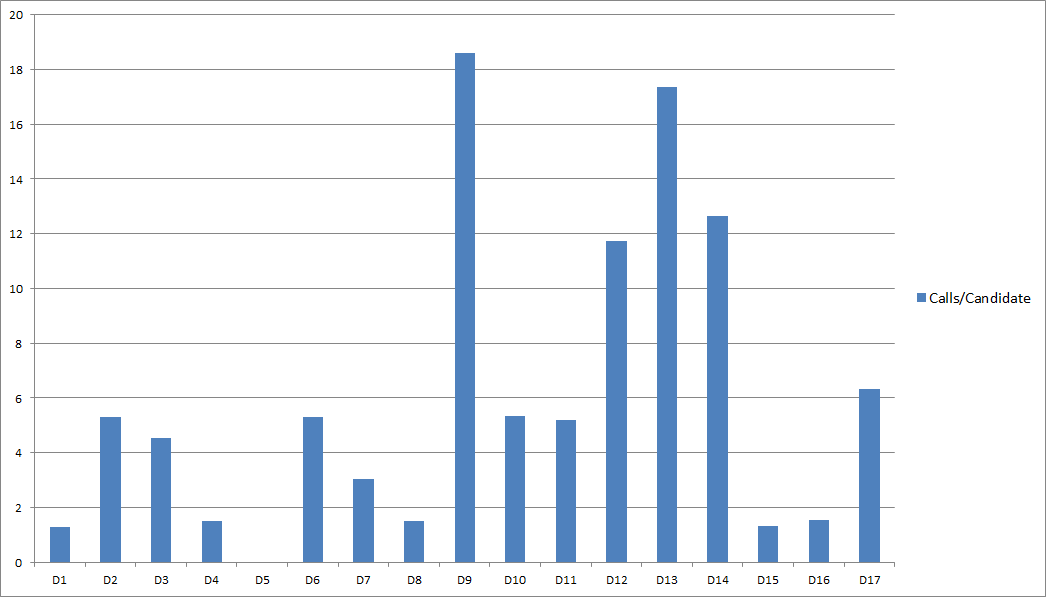
\includegraphics[width=0.9\textwidth]{media/chapter5/cx-verification-ratio-all-datasets.png}
\caption{Verification Ratio (x 100) obtained using the Context Discovery Algorithm.}
\label{fig:exp-cx-verification-ratio}
\end{figure}

In order to compare these results, we perform a tagging experiment using location information alone. Candidates are ordered according to their last known location, and presented to the user in the same style as the information presented with the context discovery algorithm. In this case, it must be noted that some users do not have location information related to them, and are excluded from the candidate set. The effect of this fact is seen in the reduced hit count seen using location information.

% \begin{figure}[ht]
% \begin{minipage}[b]{0.45\linewidth}
% \centering
% 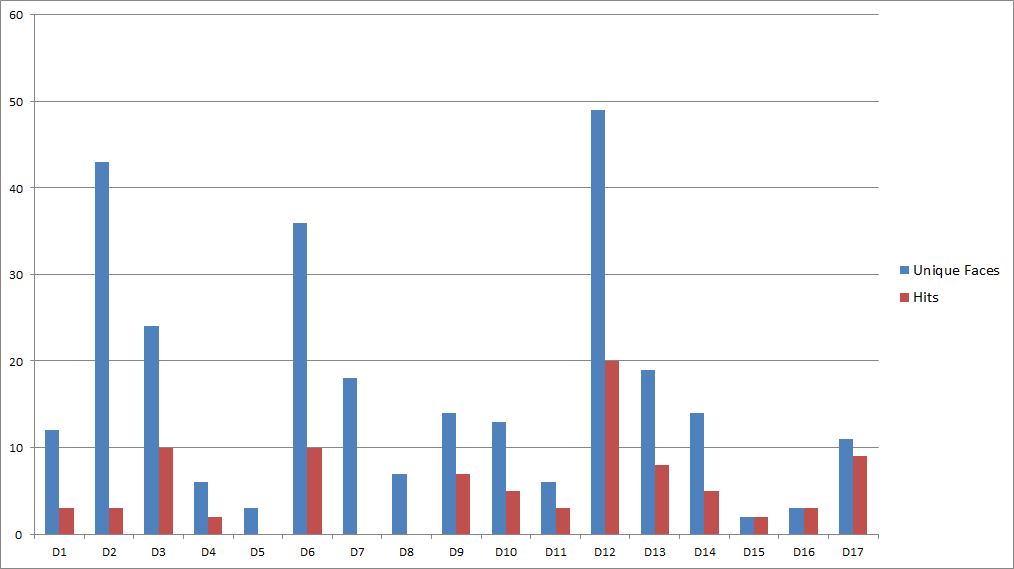
\includegraphics[width=0.9\textwidth]{media/chapter5/loc-unique-faces-hits-all-datasets.png}
% \caption{Hit counts for all datasets using Location only.}
% \label{fig:exp-loc-hits}
% \end{minipage}
% \hspace{0.5cm}
% \begin{minipage}[b]{0.45\linewidth}
% \centering
% 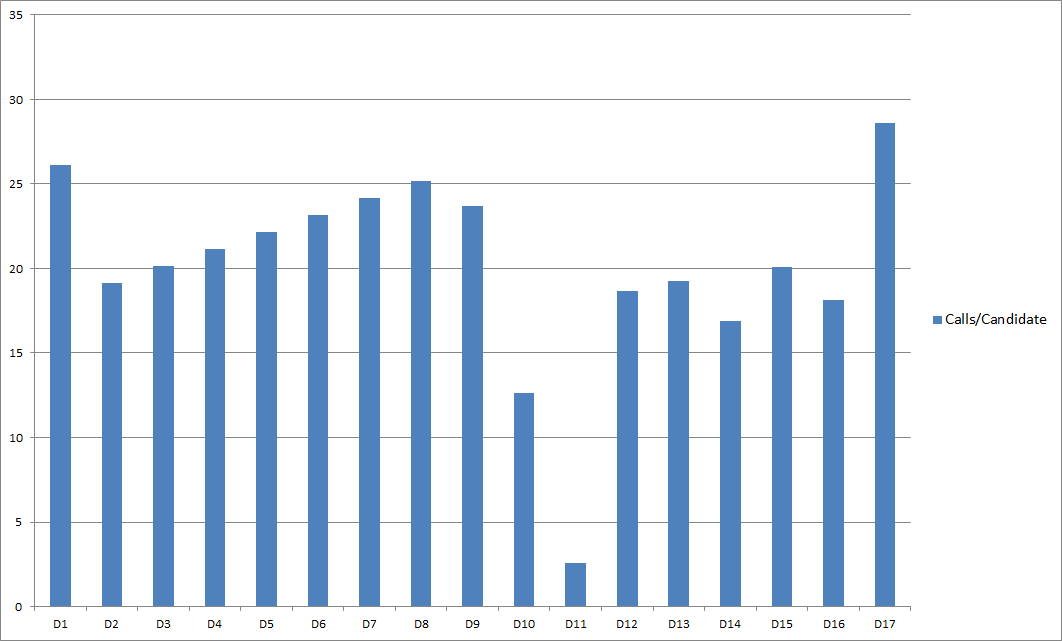
\includegraphics[width=0.9\textwidth]{media/chapter5/loc-verification-ratio-all-datasets.png}
% \caption{Verification Ratio (x 100) for all datasets obtained using Location only.}
% \label{fig:exp-loc-verification-ratio}
% \end{minipage}
% \end{figure}

\begin{figure}[ht]
\centering
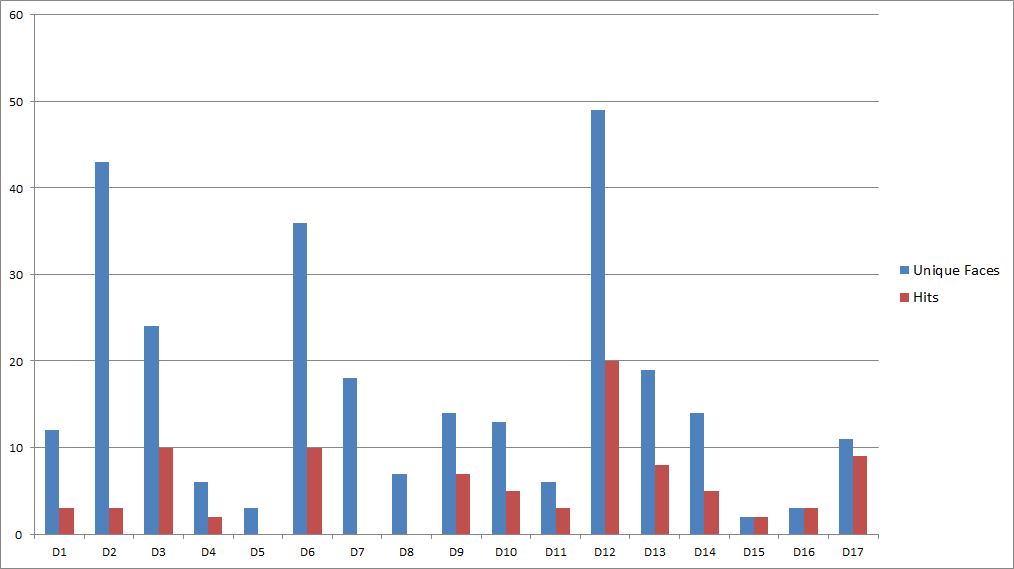
\includegraphics[width=0.9\textwidth]{media/chapter5/loc-unique-faces-hits-all-datasets.png}
\caption{Hit counts for all datasets using Location only.}
\label{fig:exp-loc-hits}
\end{figure}

Similarly, we measure the verification ratio using location only. The results in figure \ref{fig:exp-loc-verification-ratio} show that the maximum number has now increased to almost 29\%. 

\begin{figure}[h!]
\centering
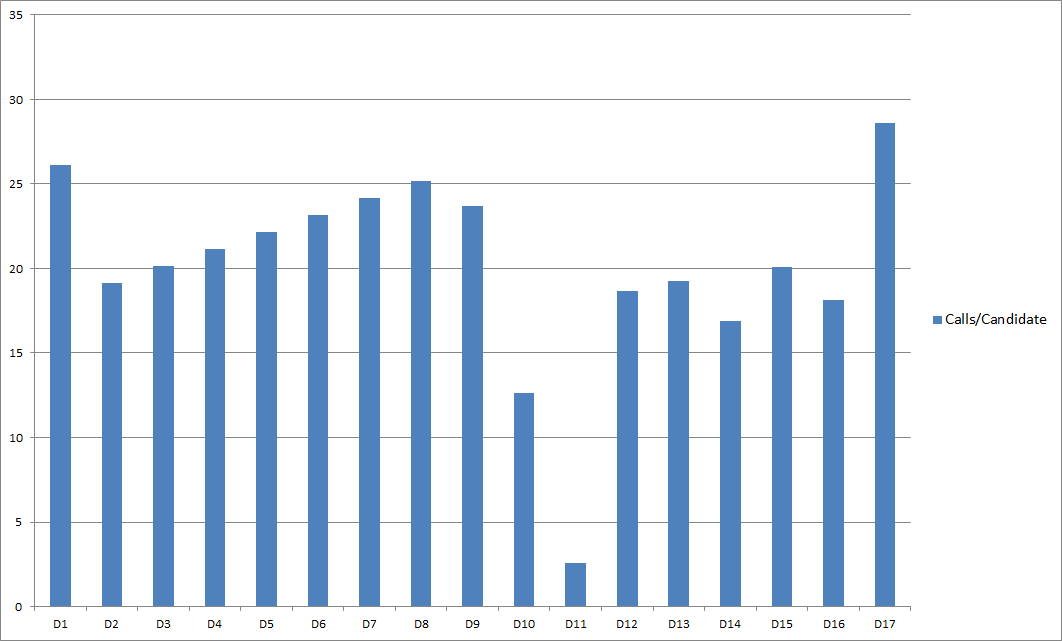
\includegraphics[width=0.9\textwidth]{media/chapter5/loc-verification-ratio-all-datasets.png}
\caption{Verification Ratio (x 100) for all datasets obtained using Location only.}
\label{fig:exp-loc-verification-ratio}
\end{figure}

\begin{figure}[t]
\centering
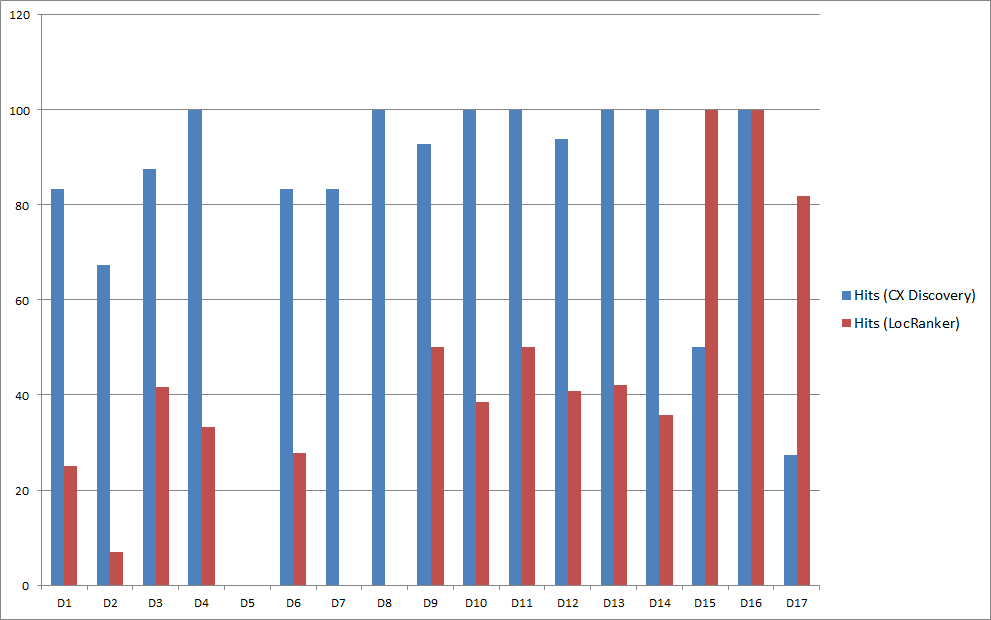
\includegraphics[width=0.9\textwidth]{media/chapter5/hits-ratio-comparison-all-datasets.png}
\caption{Comparing Hits Ratio (x 100) for all datasets.}
\label{fig:hits-ratio-comparison}
\end{figure}

In figure \ref{fig:hits-ratio-comparison}, we compare the \textbf{hits ratio} of the two algorithms. The hit ratio is the number of hits per unique face in a dataset. As it can be seen, the context discovery algorithm outperforms the simple location based ranking algorithm. The more important insight in this graph is that the context discovery algorithm performs \textbf{consistently across different types of events}, whereas the location based metric is good only for the party events. Figure \ref{fig:verification-ratio-comparison} compares the different verification ratios. The relatively lower numbers for the context discovery algorithm indicate its superior ranking over the location based algorithm. Again, the important thing is to note its \textbf{performance across event types}. 

\begin{figure}[t]
\centering
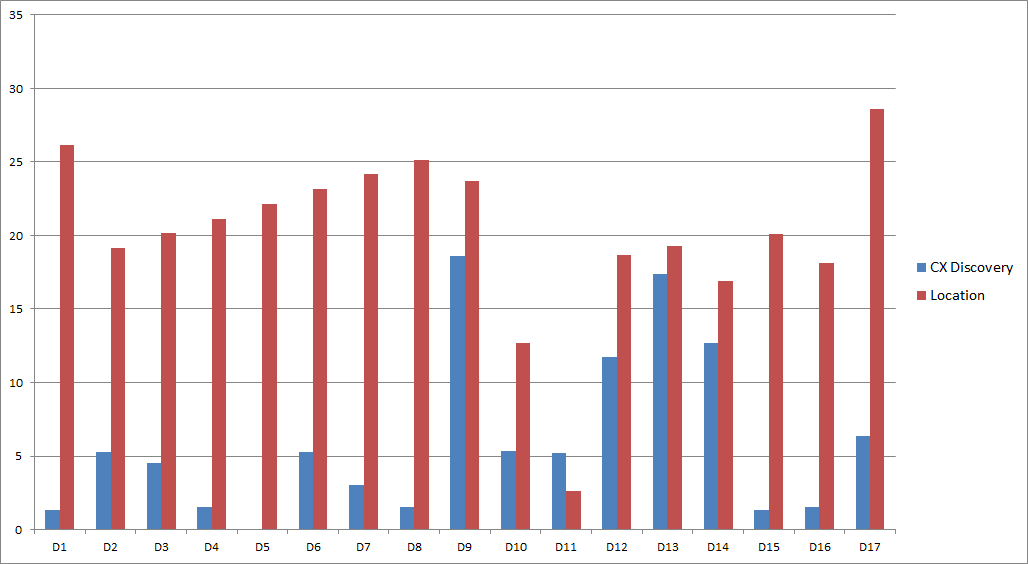
\includegraphics[width=0.9\textwidth]{media/chapter5/verification-ratio-comparison-all-datasets.png}
\caption{Comparing Verification Ratio (x 100) for all datasets.}
\label{fig:verification-ratio-comparison}
\end{figure}

\subsection{Conclusion}
We summarize the results of this experiment as follows. The context discovery algorithm performs consistently well across different types of events. Depending on the type of the event, it discovers the best data sources and ranks the candidate set in the appropriate way. For a single dataset, the ranking of candidates can significantly vary depending on who has been tagged in the photo. We have not implemented any cross-photo context propagation into our algorithm, but this is an active area of research, and there are many possible ways of introducing that technique into our context discovery algorithm.

% Now, lets look at reduction obtained in state space with the discovery algorithm. The total number of people in our experiment universe is 660. By statically linking the sources, we would expect the search space to contain 660 candidates for tagging any of the datasets. However, the context discovery algorithm reduced the size of the search space as shown in table \ref{tbl:search-spaces}. The search space varies from 7 people in D7 (1\%) to 338 people in D2 (51\%). We denote the term hit rate as the percentage of true positives in the search space. Even if our search space is small, it might contain no annotations from the ground truth, leading to poor classifier performance. The hit rates are also summarized in table \ref{tbl:search-spaces}. For D4, the algorithm found no event sources (as seen in figure \ref{fig:src-cand-distribution}), and therefore constructed a search space which was too small, thereby containing none of the ground truth. With the exception for D4, the hit rate is always above 83\%. We observe an overall reduction in the search space size, with a high hit rate for majority of the datasets. 

% \begin{table}[h]
% \begin{center}
% \begin{tabular}{ |c|p{2.5cm}|c| }
%   \hline
%   \texttt{Dataset} & \texttt{Reduced Search Space Size} & \texttt{Hit Rate}\\
%   \hline
% %  D0 & TBD & TBD \\
%   D1 & 42 & 83.72\%\\
%   D2 & 338 & 87.5\%\\
%   D3 & 231 & 100\%\\
%   D4 & 1 & 0\%\\
%   D5 & 254 & 83.33\%\\
%   D6 & 20 & 88.89\%\\
%   D7 & 7 & 100\%\\
%   \hline
% \end{tabular}
% \caption{Sizes of Search Space for each dataset.}
% \label{tbl:search-spaces}
% \end{center}
% \end{table}

% We now investigate the role of different context sources in the discovery algorithm. If an entity in the search space was merged into the event graph by an event source, they are said to be ``contributed" from it. We profiled our algorithm to log all contributions which were true positives for the classification algorithm. Figure \ref{fig:tag-distribution} shows the contribution from various sources for all datasets. For example, D1 obtained 69.77\% of true positives in its search space from event sources, 2.33\% from personal information and 11.63\% from social networks. 16.28\% of true positives for D1 were obtained from no source, and were therefore marked as ``Out of Context Network". 

% This graph brings to light our argument that most of the true positives, for all datasets, were obtained as a result of navigating the event sources. It will also be noted that the role of social networks is minimal. It was found useful for only one dataset. Relying on social networking sources would have led to a large number of false positives in the classifier performance. Even though the role of personal information is negligible, it is critical in linking in photos to the owner, and from there to different events. Without the availability of personal information, the algorithm would not have reached the context rich event sources.

% % the lower selection of candidates shows the selectivity of CueNet in extracting information from different sources. Because it constructs queries with as many predicates as possible, the availability of time and space prompts it to navigate event sources more than social networking sources.

% \begin{figure*}[t]
% \centering
% 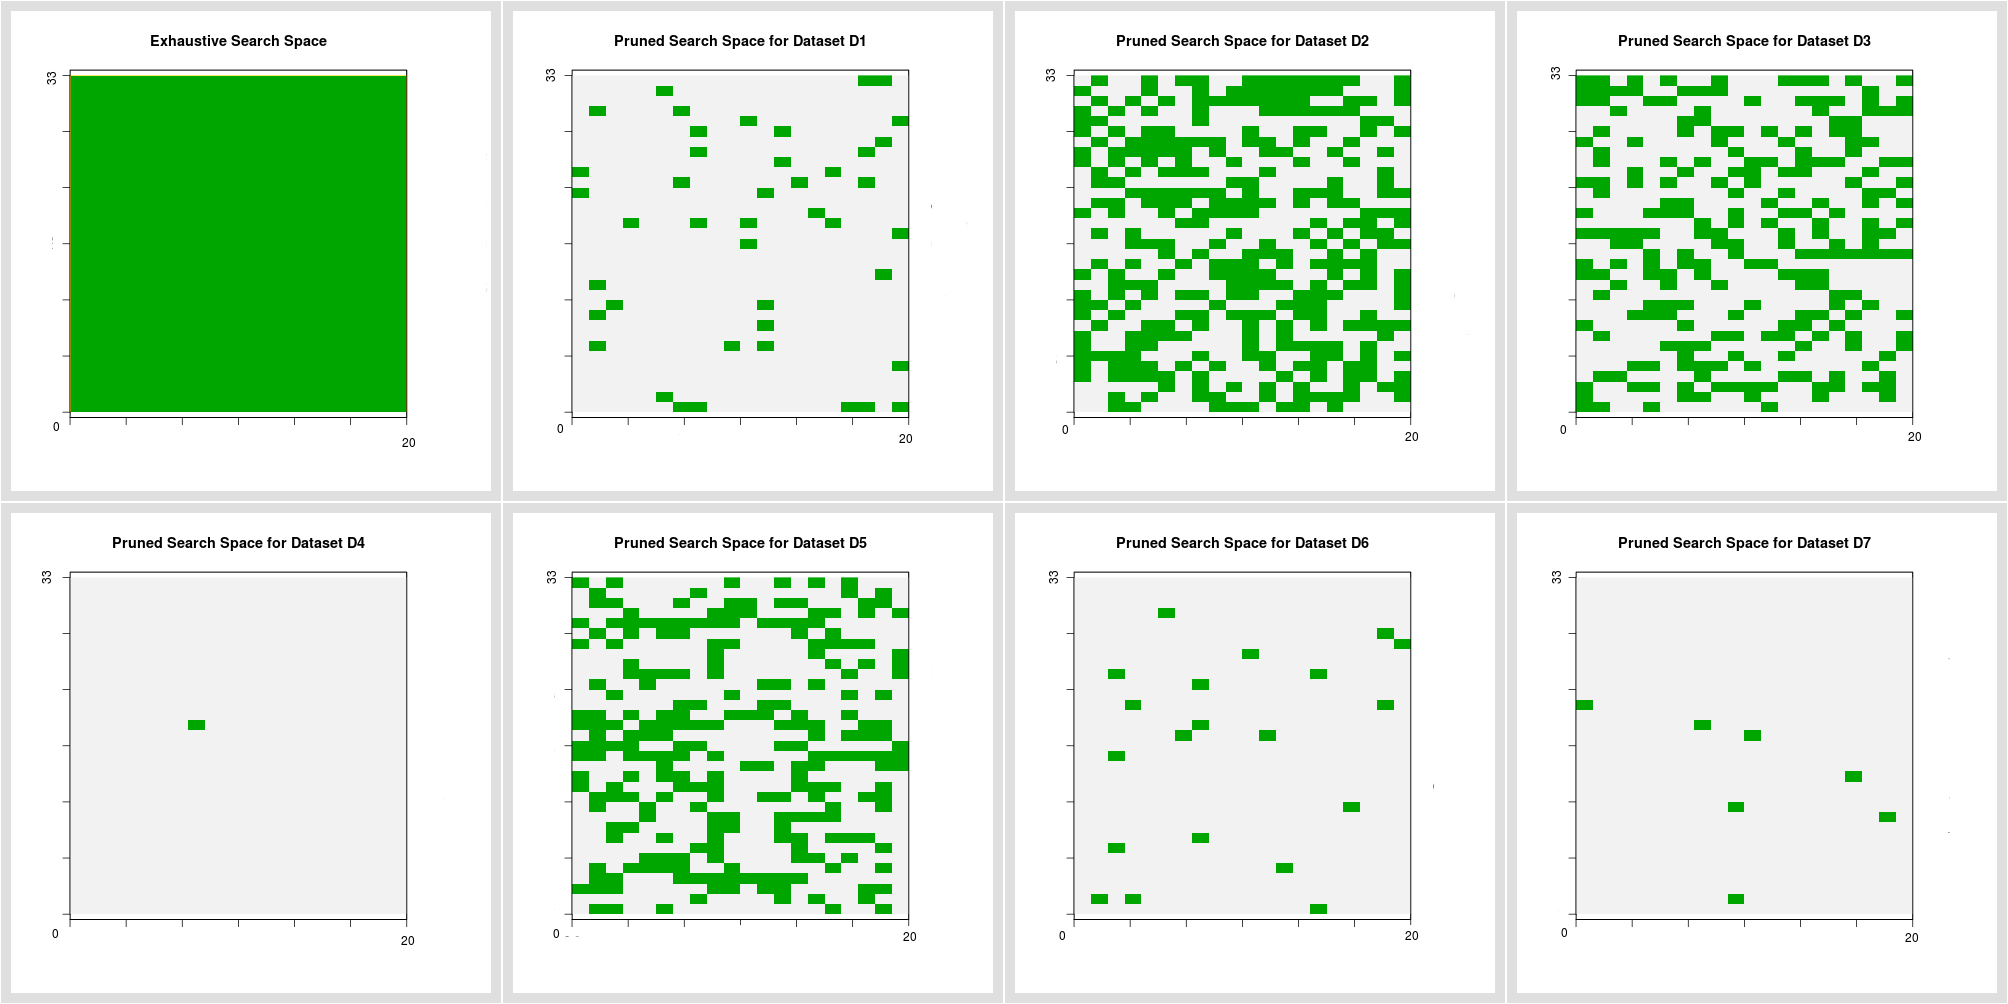
\includegraphics[width=\textwidth]{diversity/montage-clean-pruned-labelled.png}
% \caption{Grid plots showing the exhaustive search space and pruning in search space for different datasets.}
% \label{fig:diversity}
% \end{figure*}

% \subsection{Search Spaces}
% Finally, we compare the various search spaces constructed by discovery algorithm. We represent all people in our experiment universe in a color grid (with 33x20 cells for 660 people). Each cell represents the presence or absence of a person in the search space. If a person was present in the candidate list provided to the tagging algorithm, we color the corresponding cell green, otherwise it is colored white. Figure \ref{fig:diversity} shows the color grids describing search spaces for all datasets, and an exhaustive search space. The positioning of people along the grid is arbitrary, but consistent across grids. Our aim in this visualization is to see the diversity in search spaces created by the algorithm. The purpose of the exhaustive search space is to provide easy comparision to appreciate the reduction in search space. 

% It can be seen that CueNet prunes the search space very differently for different datasets. As we move from dataset to dataset, the data sources present different items of information, and therefore CueNet constructs very search spaces. Dataset D2, D4 and D5 are very large conferences hosting hundreds of people in the same field. This explains why a large portion of the grid is covered. Also, this was the same conference held in three different years, and therefore, had a lot of common attendees resulting in overlap.

% \begin{figure}[t]
% \centering
% 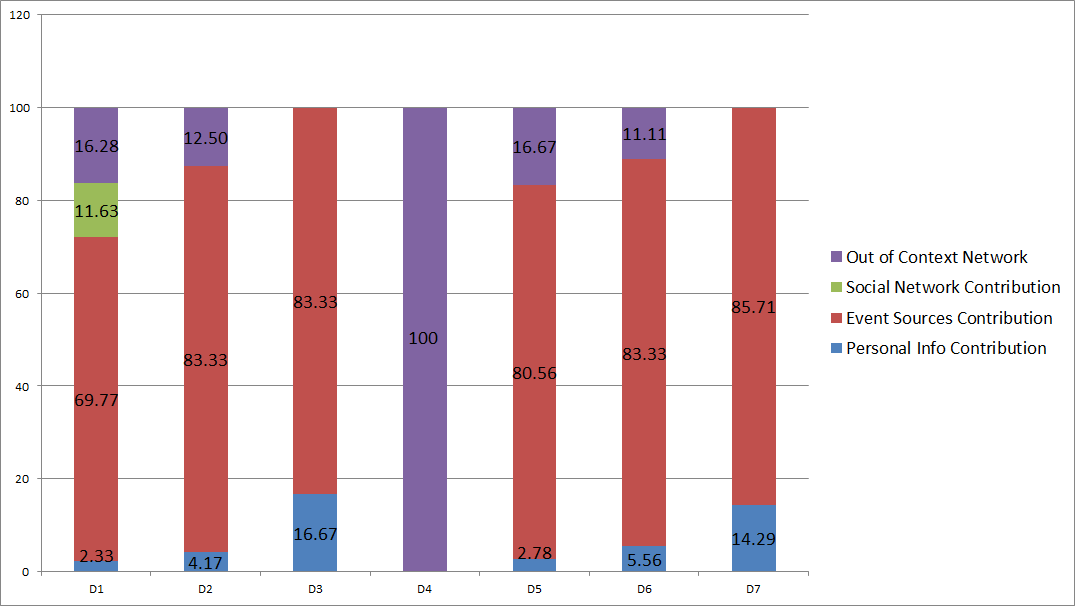
\includegraphics[width=0.9\textwidth]{media/discovery-distro-stacked-2.png}
% \caption{Graph showing the contribution of each source type in context discovery.}
% \label{fig:tag-distribution}
% \end{figure}

% \subsection{Conclusion}
% These experiments validate our three hypotheses. \textbf{First}, Event sources contain a large portion of true positives. From 70\% in D1 to 100\% in D7. There are events for which there is no documentation, and event sources are not able to contribute anything here, as in the case of D4. \textbf{Second}, the discovery algorithm is able to prune the search space using event, personal and social information. The reduction is atleast 50\% for D2 (338 candidates out of 660) but can be very large in some cases (7 candidates for D7). \textbf{Third}, The reduced search space retains a high number of true positives. The hit rate is between 83\% to 100\% (with the exception of D4, where the search space provided no true positives). We also saw how unique the search spaces are, to each dataset, thereby demonstrating the dynamic nature of the algorithm.

\section{Performance Analysis}
In this section, we will look at the performance characteristics of the CueNet algorithm. More specifically, the merge function in the discovery algorithm. In order to achieve this, we will present a generative model to generate large workloads of context networks, which will be merged with each other. Using the generative model, networks of varying sizes will be created so that the time and space complexity of the algorithm can be studied.

\subsection{Generative Models}
The generative model requires three main components. A set of places where events occur. An ontology which determines what events occur, and how certain events are more likely to occur as sub-events of already occurring events and the event instances themselves. We will describe each of the components in turn. 


\begin{figure}[t]
\centering
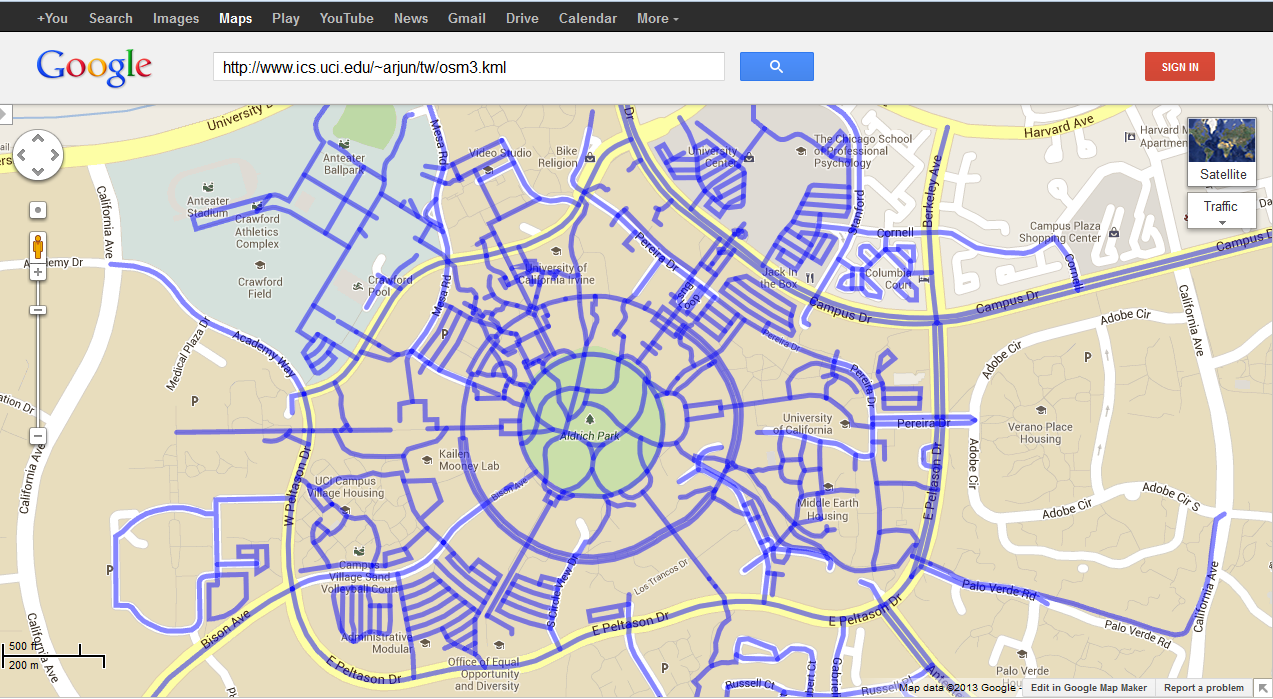
\includegraphics[width=0.9\textwidth]{media/chapter5/perf/map-locations.png}
\caption{Roadmap containing places where events could occur.}
\label{fig:osm-roadmap-uci}
\end{figure}

A large number of road network databases are available online. Instead of designing a generative model for places, it is advisable to use one of these real world databases and select a sample of it to obtain a list of places where events can occur. Some commonly used databases are shapefiles \cite{esri:tigerline} for road network information about a particular area. Stanford's SNAP database contains the entire road networks of the USA \cite{stanford:snap}. The FSU dataset available at \cite{fsu:spatial} provides detailed road networks with GPS coordinates from various parts of the country. For our work, we found the spatial database available from OpenStreetMap as the best resource. Their database provides information about road networks, as well as the places themselves. At the same time, road maps can be downloaded from their website using the download tool or maps for entire cities or states or countries can be downloaded from \cite{cloudmade:download}. The road map of UCI downloaded from their website and converted to KML format is shown in figure \ref{fig:osm-roadmap-uci}. The map data also contains information about different types of objects which can be found on these roads. Please look at their extensive taxonomy \cite{osm:taxonomy} regarding what types of objects can be found here. We select a sample of the nodes in such a network to be our place set.


\begin{figure}[t]
\centering
\includegraphics[width=0.9\textwidth]{media/chapter5/perf/gaussian-split.png}
\caption{Gaussian distribution split to generate randon events in ontology.}
\label{fig:gaussian-split}
\end{figure}


The ontology generation module provides three parameters. $O_d$, which controls the depth of subevent trees. $O_{ms}$ which is the maximum number of subevents an event can have. $D$, which is the distribution type. The distribution type decides which events are selected into a hierarchy. A distribution could be Gaussian or Poisson or Uniform distribution. Once the distribution is selected, parameters of the distribution are also provided. We will use a Gaussian distribution as an example to explain the generation of ontologies. But the ideas can be applied to any kind of distribution. 

We want to model events into three categories depending on their generate rate of occurrence. Some events are very commonly occurring, a majority of events occur average number of times, and events in the third category occur very rarely. Figure \ref{fig:gaussian-split} shows how a gaussian random value generator can be used to bucket events into these three zones. The random values are compared with the values $a$, $b$ and $c$. If the $|value|$ is between 0 and $a$, then the event falls into the first category. If it lies between $a$ and $b$, then it lies in the second category. Otherwise it is in the third category.

We consider events in the first category to be atomic events. That is, they occur independently and do not have a subevent hierarchy. An example could be a tweet event or a \texttt{photo-capture} event. We want to create two types of hierarchies. One which is short and fat, and the other which is long and tall. We choose category two to correspond to the former, and category three to contain the latter type of hierarchies. A hierarchy is generated as follows: choose an event, if it is from category 2 or 3, a hierarchy with atmost depth $O_d$ and each super event having max $O_{ms}$ subevents is generated. The events are randomly chosen based on their ``real-world'' frequency. These hierarchies are serialized into files. For events in category 3, we double the value of $O_{ms}$. This will allow us to get \textit{fatter} instance hierarchies as we will see later.

In order to generate instances, we randomly select an event based on its ``real-world'' frequency, and load the hierarchy structure from the file, and for subevent class, generate $n$ instances. Thus, if an event $x$ has a subevent $y$ in its hierarchy, then the instance $x_i$ will have subevent instances $\{y_1, y_2 ... y_{|Y|}\}$ where $|Y| < n$. The number $n$ is decided on the basis of an input metric $C$, where for events in category 2, $n = c/2$, and for events in category 3, $n = C$. It must be noted that the $n$ is the maximum number of subevents a super event can contain. The actual number of subevent instances is decided by a uniform random number generator. These hierarchies are serialized into files and stored for the merge tests.

\subsection{Procedure}
In order to understand the time and space complexity of the merge function, we load multiple networks from instance hierarchy into in-memory data structures, and perform a sequence of merges. In order to simulate the workload similar to the discovery algorithm, we select a network, and perform a sequence of merges on it. We will refer to the initially selected network as a \textbf{primary} network and the networks which are merged into it as \textbf{secondary} networks. Thus, given a primary network and a set of secondary networks, we perform the following set of experiments.

First, we fix the size of the primary networks (in terms of node count), and merge secondary networks with varying size, and measure the time taken for the merges to complete.

Second, we fix the size of the primary networks (in terms of depth), and merge secondary networks with varying depth, and measure the time taken for the merges to complete.

Third, we merge a context network with an exact replica of itself, and measure the time taken for the operation. We also change the size of the heap size, and see if there is any effect on the merge operation.

Fourth, we measure the sizes of the networks once they are in memory.

It must be noted that the event instances being used in the experiments do not have event metadata associated with the in-memory instance object. It is assumed that these are being stored separately. The networks used below are simply events with type, spatio-temporal and identification information and references to their subevents and to entities who participate in the events. Any additional information, for example the image object which constitutes the experiential aspect of an event, is stored separately.

We use the following system setup in all our experiments. We use a 8 core Intel(R) Xeon(R) E5504 processor clocking at 2.01Ghz with 8 gigabytes of main memory. We use a single thread to load networks from the file on the disk and proceeds to merge them. The memory footprints of the networks are measured by the classmexer library \cite{classmexer}. The \texttt{Xmx} and \texttt{Xms} JVM parameters were set to be 6000m and 256m respectively.

\begin{figure}[t]
\centering
\includegraphics[width=0.9\textwidth]{media/chapter5/perf/mergebignodetest.png}
\caption{Graph showing merge times for different sizes of primary networks.}
\label{fig:agg-merge-tests}
\end{figure}

\subsection{Results}
The graph shown in figure \ref{fig:agg-merge-tests} shows the time taken for merging secondary networks of increasing sizes to a primary network. The size of the primary network is increased from 10 nodes to a million nodes. For each such primary network, a number of secondary networks are merged. As we can see, the size of the primary network does not contribute to the time complexity of the algorithm. This is because the merge algorithm effectively searches the subevent structure to find the node which can best accommodate the secondary network. This is a walk down a single path of the tree. Thus, as long as small secondary networks are obtained from the sources, the merge operations will be less expensive. This is the reason why we tailor our discover queries to provide only very specific information. On the other hand, as the  size of the secondary network increases, we find that the performance increases linearly upto a point, after it which it exponentially increases. This is due to a combination of tree traversal on the secondary network, and the JVM's garbage collector removing outdated objects to accommodate the new objects being created in the primary network. In our implementation, we create new objects in the primary network, as opposed to copying them from the secondary network.

\begin{figure}[t]
\centering
\includegraphics[width=0.9\textwidth]{media/chapter5/perf/mergedepthtest.png}
\caption{Time to merge networks with varying depth.}
\label{fig:agg-depth}
\end{figure}

Similarly, in figure \ref{fig:agg-depth}, we test how merge time varies with increasing depth of the primary network. Here we fix the depth of the primary network to 3, 5 or 7 levels, and load a set of secondary networks from depth 1 to 9. The secondary networks are merged in sequence to the primary network. Each run of the algorithm corresponds to a single primary network (effectively, we reboot the JVM for each primary network). Here the exponential rise after the depth of the secondary network reaches 8 levels is more obvious. This again, shows the importance of constructing selective queries during the discover phase of the algorithm. The loading of all the secondary networks prior to the merge sequence allows us to study the cost of merges in an environment where  memory is not available, and is shared by other citizen objects of the JVM heap. 

Figures \ref{fig:1k-self-merge} and \ref{fig:1m-self-merge} show the time complexity of self merges. A self merge is merging a network with an identical copy of itself. The perforance characteristics are very similar to the merge tests seen before.

\begin{figure}[ht]
\begin{minipage}[b]{0.45\linewidth}
\centering
\includegraphics[width=\textwidth]{media/chapter5/perf/selfmerge_10K.png}
\caption{1K-10K Nodes Self Merge}
\label{fig:1k-self-merge}
\end{minipage}
\hspace{0.5cm}
\begin{minipage}[b]{0.45\linewidth}
\centering
\includegraphics[width=\textwidth]{media/chapter5/perf/selfmerge_1M.png}
\caption{100K-1M Nodes Self Merge}
\label{fig:1m-self-merge}
\end{minipage}
\end{figure}

\begin{figure}[t]
\centering
\includegraphics[width=0.9\textwidth]{media/chapter5/perf/selfmerge-increasing-xmx.png}
\caption{Time to merge networks with varying available heap space.}
\label{fig:agg-xmx}
\end{figure}


Now, we will look at how the merges behave with varying heap size (the \texttt{Xmx} runtime parameter provided to the JVM when it is initialized). In figure \ref{fig:agg-xmx}, we see 5 different curves, corresponding to \texttt{Xmx} values of 512m, 640m, 768m, 896m, and 1024m. We load a network twice, perform a merge (a \textit{self-merge}), and record the time the operation takes. The experiments is repeated 5 times for each merge on different randomly created networks. We perform these operations on networks containing 1000, 2000, 3000 nodes upto 700K, 800K, 900K and 1M nodes. As we can see in the figure, we run out of heap space when the networks contain 600K and the Xmx value is 512m. Beyond a 896m, we see that the merge operations only grow linearly, and can be considered a safe limit when self-merges of 1M node networks are to be performed. For heap spaces of less than 896m, the performance time increases exponentially when the network size exceeds 600K nodes. This is, again, because of the creation of nodes in the primary networks.

Finally, we use the Classmexer library \cite{classmexer} to measure the memory footprint of the in-memory context network. We generate random networks of size 1000, 2000 ... 10,000 nodes, and measure the size in kilobytes. The results are shown in figure \ref{fig:sizes}.

\begin{figure}[t]
\centering
\includegraphics[width=0.9\textwidth]{media/chapter5/perf/size-tree-1000.png}
\caption{Sizes of in-memory context networks contain a few thousand nodes.}
\label{fig:sizes}
\end{figure}


\subsection{Conclusion}

In analysing the above figures, we have seen that the in-memory merge algorithm performs very well for networks upto 500K nodes. Beyond this point, the performance exponentially decays, both as a combination of large graphs, and the JVM's garbage collector trying to clean up unwanted objects. And therefore it is best recommended to approach an disk based solution or partition the context networks across different machines. 

Since performing many merges (especially with large secondary networks), it is advisable to not perform the merges when the rate of incoming networks is very high. Rather, the system can cache the networks, and utilize techniques like iterative dynamic programming or \textit{batch} the merges such that the overall load on the CPU is reduced. Such an algorithm, to the best of my knowledge, does not readily exist, and can be a very fruitful future research to improve the utility of context networks in various domains.

% \begin{figure}[ht]
% \begin{minipage}[b]{0.45\linewidth}
% \centering
% \includegraphics[width=\textwidth]{media/chapter5/perf/mergebignodetest_10.png}
% \caption{10 Nodes}
% \label{fig:pic1}
% \end{minipage}
% \hspace{0.5cm}
% \begin{minipage}[b]{0.45\linewidth}
% \centering
% \includegraphics[width=\textwidth]{media/chapter5/perf/mergebignodetest_100.png}
% \caption{100 Nodes}
% \label{fig:pic2}
% \end{minipage}

% \begin{minipage}[b]{0.45\linewidth}
% \centering
% \includegraphics[width=\textwidth]{media/chapter5/perf/mergebignodetest_1000.png}
% \caption{10 Nodes}
% \label{fig:pic1}
% \end{minipage}
% \hspace{0.5cm}
% \begin{minipage}[b]{0.45\linewidth}
% \centering
% \includegraphics[width=\textwidth]{media/chapter5/perf/mergebignodetest_10K.png}
% \caption{100 Nodes}
% \label{fig:pic2}
% \end{minipage}

% \begin{minipage}[b]{0.45\linewidth}
% \centering
% \includegraphics[width=\textwidth]{media/chapter5/perf/mergebignodetest_100K.png}
% \caption{100K Nodes}
% \label{fig:pic2}
% \end{minipage}
% \hspace{0.5cm}
% \begin{minipage}[b]{0.45\linewidth}
% \centering
% \includegraphics[width=\textwidth]{media/chapter5/perf/mergebignodetest_1M.png}
% \caption{1M Nodes}
% \label{fig:pic3}
% \end{minipage}
% \end{figure}


% \begin{figure}[ht]
% \begin{minipage}[b]{0.28\linewidth}
% \centering
% \includegraphics[width=\textwidth]{media/chapter5/perf/mergedepthtest_3.png}
% \caption{depth = 3}
% \label{fig:pic1}
% \end{minipage}
% \hspace{0.5cm}
% \begin{minipage}[b]{0.28\linewidth}
% \centering
% \includegraphics[width=\textwidth]{media/chapter5/perf/mergedepthtest_5.png}
% \caption{depth = 5}
% \label{fig:pic2}
% \end{minipage}
% \hspace{0.5cm}
% \begin{minipage}[b]{0.32\linewidth}
% \centering
% \includegraphics[width=\textwidth]{media/chapter5/perf/mergedepthtest_7.png}
% \caption{depth = 7}
% \label{fig:pic3}
% \end{minipage}

% \end{figure}
\chapter{Tag Propagation}

So far, our treatment of context networks deals exclusively with context from external data sources. But similar groups of people participate in similar kinds of events. For example, attending meetings with colleagues, attending parties with friends and attending similar concerts with people who share similar musical tastes . We will explore how past participation information can be used to rank candidates for a new event.

In this chapter, we will attempt to address this problem of boosting the performance of the CueNet framework by introducing a technique to rank candidates based on their participation profile in neighboring context networks, personal interests or relation with other participants. We will present our intuition through a series of examples, and introduce a technique similar to PageRank, which is used to rank pages on the world wide web. In our case, we will rank people in the \texttt{CandidateSet} given set of context networks. Our main differences will lie in the initialization of the score matrix and the propagation of scores \textit{across} the different context networks using event semantics. We will use properties of events such as temporal, spatial and type properties to score candidates for events.

\section{Preliminaries}

Rank propagation techniques have been used to rank nodes in directed graphs. Most commonly seen versions in today's literature are the HITS algorithm invented by Jon Kleinberg \cite{kleinberg1999authoritative} and the PageRank algorithm developed by Larry Page and Sergey Brin \cite{page1999pagerank}. The idea in the latter is to assign a set of initial values to a subset of nodes, and propagate a fraction of these values to their neighbors. Each iteration of the algorithm propagates their scores to the neighboring nodes until the overall ordering of the nodes, according to their scores, does not change. In practice, a few iterations ($<$ 100) on web scale graphs is sufficient to achieve convergence.

\begin{figure}[t]
\centering
\includegraphics[width=0.65\textwidth]{media/chapter6/pr-example-graph.png}
\caption{Example graph to demonstrate the original Pagerank algorithm.}
\label{fig:pr-graph-example}
\end{figure}

The page rank \cite{page1999pagerank} algorithm, designed to rank large nodes in web graphs is an extension of this idea. The intuition behind page rank is that of the random surfer model. The rank propagation models the behavior of a random web surfer who follows a few links and then gets `bored' and jumps to a random part of the web graph. The final scores of the ranking algorithm converge to the probabilities of such a surfer spending time at a particular page. Another analogy to understand PageRank would be the following: If many surfers (where number of surfers is greater than number of nodes) uniformly choose a page to start surfing from, and move to either one of the outgoing nodes or decide to jump to another page in the graph, then after some iterations, the page rank of a node is fraction of surfers left on it. Mathematically, the page rank of a given web page $i$ at the $k^{th}$ iteration of the rank computation algorithm, denoted as $PR(i, k)$ is defined recursively according to the equation \cite{borodin2001finding}:

\begin{align}
\label{eq:pagerank}
% PR(i) = dD(i) + (1 - d) \sum_{j \rightarrow i} [PR(j)/N(j)] \\  %Equation from Borodin's paper
PR(i, k) = dD(i) + (1 - d) \sum_{j \rightarrow i} [PR(j, k - 1)/N(j)]
\end{align}

In equation \ref{eq:pagerank}, $d$ is the probability with which the random surfer will jump to a sample from the distribution $D(.)$, and with probability (1-d) jumps uniformly at random to one of the pages linked from the current page.

\restylealgo{ruled}
\SetAlgoSkip{}
\begin{algorithm}[t]
\dontprintsemicolon 
\Begin{
  
$R_0$ $\leftarrow$ S  \\
\textbf{loop}: \\
\Indp
  $R_{i+1}$ $\leftarrow$ $AR_i$ \\
  d $\leftarrow$ $||R_i||_1$ - $||R_{i+1}||_1$ \\  
  $R_{i+1}$ $\leftarrow$ $||R_i||_1$ + dE \\
  $\delta$ $\leftarrow$ $||R_{i+1} - R_i||_1$ \\
\Indm
\textbf{while $\delta > \epsilon$}
}
\caption{Original Pagerank Algorithm}
\label{alg:pr-alg}
\end{algorithm}

Let us take a look at how rank propagation works in simple graphs. Consider the directed graph in figure. Let the initial scores of all nodes be 0.25. In the first iteration of the algorithm, if we assume that the surfer will only follow links (i.e., d = 0), the score of node A would be computed as follows. Since A has two incoming edges from B and C, they will transfer a portion of their scores to A. Since B has two outgoing edges, it will transfer half of its score to A. C has only one outgoing edge, and therefore transfers all of its score to A. Thus, the value $PR(A)$ becomes $0.25/2 + .25 = 0.375$ at the end of the first iteration. Similarly, B obtains half the score of D; C obtains half of B and half of D; and D obtains the full score of A. For each node, we can rewrite \ref{eq:pagerank} as follows:

\begin{flalign}
\label{eq:p1}
&PR(A, i) = \frac{PR(B, i-1)}{2} + PR(C, i-1) & \\
&PR(B, i) = \frac{PR(D, i-1)}{2} & \\
&PR(C, i) = \frac{PR(D, i-1)}{2} + \frac{PR(B, i-1)}{2}& \\
&PR(D, i) = PR(A, i-1) & 
\end{flalign}

If the probability of jumping to a web page from the distribution D is 0.15, and we assume that the probabilities in $D$ are equally likely, the above equation to compute the new pagerank of node A becomes $PR(A, i) = \frac{d}{N} + (1-d)\frac{PR(B, i-1)}{2} + PR(C, i-1) = 0.35625$. Table \ref{tbl:prc} shows the different values of page rank for each node in our example graph per iteration until it converges. We assume that the initial ranks of each node is 0.25. The difference in ranks is computed using L1 norm of the difference of ranks in the current and previous iteration.

\begin{flalign}
\label{eq:norm}
\delta = \sum_{\forall i}{|PR(i)  - PR(i-1)|}
\end{flalign}

\begin{table}[h]
\begin{center}
\begin{tabular}{ |c|c|c|c|c|c| }
  \hline
  \texttt{k} & \texttt{A} & \texttt{B} & \texttt{C} & \texttt{D} & \texttt{$\delta$}\\
  \hline
  1  &  0.25000  &  0.25000  &  0.25000  &  0.25000  &  - \\
  1  &  0.35625  &  0.14375  &  0.25000  &  0.25000  &  0.21250 \\
  2  &  0.31109  &  0.14375  &  0.20484  &  0.34031  &  0.18062 \\
  3  &  0.27271  &  0.18213  &  0.24323  &  0.30193  &  0.15353 \\
  4  &  0.32165  &  0.16582  &  0.24323  &  0.26930  &  0.09788 \\
  5  &  0.31472  &  0.15195  &  0.22243  &  0.31090  &  0.08319 \\
  6  &  0.29114  &  0.16963  &  0.23421  &  0.30501  &  0.05893 \\
  7  &  0.30868  &  0.16713  &  0.23922  &  0.28497  &  0.04508 \\
  8  &  0.31187  &  0.15861  &  0.22964  &  0.29987  &  0.03619 \\
  9  &  0.30011  &  0.16495  &  0.23236  &  0.30259  &  0.02352 \\
  10 &  0.30511  &  0.16610  &  0.23620  &  0.29259  &  0.02000 \\
  ... &  ...  &  ...  &  ...  &  ...  &  ... \\
  34 &  0.30554  &  0.16381  &  0.23343  &  0.29721  &  0.00002 \\
  35 &  0.30554  &  0.16382  &  0.23344  &  0.29721  &  0.00002 \\
  36 &  0.30554  &  0.16381  &  0.23344  &  0.29721  &  0.00001 \\
  37 &  0.30554  &  0.16381  &  0.23343  &  0.29721  &  0.00001 \\
  38 &  0.30554  &  0.16381  &  0.23344  &  0.29721  &  0.00001 \\
  39 &  0.30554  &  0.16381  &  0.23344  &  0.29721  &  0.00000 \\
  40 &  0.30554  &  0.16381  &  0.23343  &  0.29721  &  0.00000 \\
  \hline
\end{tabular}
\caption{Page rank scores for nodes in the example graph per iteration using equation \ref{eq:pagerank} (d = 0.15). We observe convergence of node scores after iteration 39.}
\label{tbl:prc}
\end{center}
\end{table}

The page rank algorithm is shown in algorithm \ref{alg:pr-alg}. R is a vector over all the nodes in the graph. A is an adjacency matrix where each cell measures is the reciprocal of outgoing edge count. If $u$ and $v$ are two nodes, and there are $N_u$ outgoing edges from $u$ and one of them ends in $v$, then $A(u, v) = 1/N_u$. The expression $||R||_1$ is the L1 or Manhattan norm of a vector $R$, which is computed as $\sum_{\forall i} |R_i|$. The vector $S$ is the initial score assigned to the nodes. On a large scale, pagerank scores are computed using the MapReduce framework \cite{dean2008mapreduce}. Each iteration of the computation corresponds to one map reduce job. Multiple such iterations are performed to obtain the final results.

\section{Intuition}

To rank objects in context networks, we modify the random surfer model slightly to model the movement of objects between different networks. Consider a set of context networks, each of which correspond to a \texttt{photo-capture-event}. Each network consists of a set of participating objects. An object in a particular network can move to a neighboring context network depending on the differences between properties of the two networks. If the two photos were captured right next to each other, and contain very similar types of events, and object instances, then there is a high probability that this person who was tagged in one of them, will be present in the other. Time is one such axis of propagation. Other properties such as event class, object co-occurrence, place (type of place or the distance) of event occurrence or subevent patterns in context network can provide different axes to propagate tags between photos.

\begin{figure}[t]
\centering
\includegraphics[width=0.65\textwidth]{media/chapter6/time-example-2.png}
\caption{Score map for events $E_1$ to $E_7$ with candidate persons $P_1$ to $P5$. Score 1 is assigned if a person was participating in the event, and a 0 if not.}
\label{fig:time-example}
\end{figure}

Consider the context networks shown in figure \ref{fig:time-example}. Events \texttt{E1} - \texttt{E7} contain one or more persons from the candidate set \texttt{P1} - \texttt{P5}. The binary vector below event describes whether an object was present in the event or not. \texttt{P1}, for example, participates in \texttt{E1} and \texttt{E2}. \texttt{P5} participates in events \texttt{E4} through \texttt{E7}. The top row shows the time of occurrence for all events. We shall assume that other properties of an event (class, location and subevent structure) are same, and therefore do not effect the propagation. Since \texttt{E6} contains \texttt{P4}, it can be said that there is a higer chance of \texttt{P4} participating in \texttt{E7} than in \texttt{E1} for two reasons. First, the object distribution in \texttt{E1} is very different from \texttt{E6}. \texttt{P4} has never participated in any event with the \texttt{P1} and \texttt{P2}. Second, because the temporal difference is much higher, very little can be estimated about the presence of a person in an event. If we quantify the object similarity using a set similarity measure, such as the jaccard index (represented by $d_s(e_i, e_j)$, and the effect of time using a formula $1 - \frac{\Delta T}{T_{max}}$, where $\Delta T$ is the difference between occurrence times of two events in question, represented as $d_t(e_i, e_j)$, then we can say that the score of a person will appear in some Ex at the $i^{th}$ iteration, $M(Ex, p, i)$, who is known to have appeared in some other set of events $\mathcal{E}$, where $Ex \notin \mathcal{E}$ is:

\begin{align}
\label{eq:puirank}
M(Ex, p, i) \leftarrow \sum_{e \in \mathcal{E}}[ d_t (e, Ex) d_s (e, Ex) M(e, p, i-1) ]
\end{align}

Similarly, look at figure \ref{fig:location-example} where the context networks now differ in type and location of occurrence as well. We show the event class information (indicated by `C') and location information with `L' of the event above the nodes. Their timestamps are as before, but our original assumption about spatial and ontological consistency no longer holds. Here, can we need to exploit some ontological properties about event similarities to propagate scores. If we know that \texttt{L1} is a \texttt{conference}, \texttt{L2} is a \texttt{music-event} and \texttt{L3} is a party, then can we say that \texttt{L2} events are more likely to contain the untagged person than the \texttt{conference} events. Likewise, spatial relationships propagate higher scores to objects in events which occur near each other, rather than those which occur further away.

\begin{figure}[h]
\centering
\includegraphics[width=0.65\textwidth]{media/chapter6/multi-property-example.png}
\caption{Other properties of events (space, type, subevent hierarchy patterns or object co-occurrence could be used to propagate scores.}
\label{fig:location-example}
\end{figure}

In this chapter, we will modify the page rank technique (algorithm \ref{alg:pr-alg}) to rank entities on a given set of context networks, to determine who might be participating in a new events. We will initialize scores of the nodes on the basis of what is known about the new event: the type of the instantiating class, the participating objects, and propagate the scores based on a set of propagation functions which we will introduce in the next section. Since the basic propagation algorithm is an expensive one, we will look at some ways to reduce the size of the context networks, so the algorithm converges quickly, and still provides useful results.

\section{Rank Propagation in Context Networks}

In order to rank candidates for a new given photo, we go by the observation that people participate in similar kinds of types, and spend time with similar groups of people. In other words, the distribution of people in events is not random. By ranking events, we are ordering them by some metric of similarity with respect to the context network containing the new photo. Events encapsulate heterogeneous information. Thus, their similarities must be computed across the different kinds of entities they encapsulate. For example, two event instances of the same class which have no common participating object are less similar to each other than two others which are of the same type and contain same participating objects.

For our application of face tagging, computing similar similarities across time, space, type and object information of events. In order to formalize our rank propagation mechanism, we introduce the concept of a propagation function. A propagation function will transfer score from one object in a event to itself in another event through specific property of the event. For example, if we can design a propagation algorithm around two \texttt{temporal} and \texttt{spatial} properties, scores will be transferred based only on the temporal and spatial attribute values of the events respectively. We say that the propagation function contributes a \textit{transfer ratio} across an axis. We follow the steps as shwon in algorithm \ref{alg:pr-alg} with the following differences: \textbf{First}, the vector $S$ is setup based on the distribution of persons present and the attributes of the events in the new context networks. \textbf{Second}, the matrix $A$ is computed as the product of all the transfer ratios between two events. For two events, $u$ and $w$, and propagation functions $P_t$ and $P_s$ (temporal and spatial propagations), the propagation vector is $V$ = $[P_t, P_s]$, and the score transfer vector from $u$ to $w$, $V(u, w)$ = $[P_t(u, w), P_s(u, w)]$ and the value $A(u, w)$ = $\mathcal{C} \times P_t(u, w) \times P_s(u, w)$, where $\mathcal C$ is a constant scaling factor.

\subsection{Propagation Functions}

In this section we introduce the propagation functions used in our work to rank events for the face tagging application.

\begin{itemize}
\item \textbf{Temporal Propagation}: For events $u$ and $w$, the temporal propagation function $P_t (u, w)$ propagates a fraction of the score of node $u$ to $w$ proportional to the difference between \texttt{u.duration} and \texttt{v.duration}. The transfer function can be modeled using uniform gaussian or zipf distributions. The advantage with such distributions is to model high transfer of scores who occur nearby in the temporal dimension, and ignoring those which happened too far away. The distribution parameters will be constant and set by the designer.

\item \textbf{Spatial Propagation}: Similar to the temporal propagation function, this takes into consider the spatial attributes of an event while transferring scores. The distance between two coordinates can be computed through one of three ways. First, a table based scheme which allots scores based on the address information of the event. Here, high scores are given if the two events occur in the same city in comparison to those within the same country. Second, using euclidean distance between GPS coordinates of the two events. Third, compute the actual `as the crow flies' distance between the two locations. We use the formula based on the spherical law of cosines: where the distance between two pair of coordinates d(lat1, lon1, lon2), is given by (where $\mathcal R$ is the radius of the Earth (6378 kms)):


\begin{align}
\label{eq:distance}
\mathcal R \arccos(\sin(lat1) \sin(lat2) + \cos(lat1) \cos(lat2) \cos(lon2 - lon1))
\end{align}


\item \textbf{Type Propagation}: The class of the event instance is taken into consideration to compare two events. We use the concept of ontological distance to compute the type propagation score transfer. We extend the concept of \texttt{Is-A} distance given in \cite{ranwez2006ontological}. For given a subsumption hierarchy, $a$ is an ancestor of $b$ iff there is a path between $a$ and $b$. The set of concepts having a as ancestor is denoted by $desc(a)$, while its ancestors are denoted as $ansc(a)$. The set of exclusive ancestors (if a node is an ancestor of exactly one of the two nodes) of $a$ and $b$ is denoted by $exAnsc(a, b)$. The subsumption ontological distance is defined as:

$d_{IS}(a, b) = |desc(exAnsc(a, b)) \cup desc(a) \cup desc(b) - desc(a) \cap desc(b)|$.

Events also exhibit subevent relationships. Two events could have very common subevents, but might have significant subsumption distance. In this case, we want to reduce this distance. We introduce the subevent distance as the number of common subevents as the number of common descendant in the subevent hierarchy of the ontology. For a node $a$, $subdesc(a)$ is the set of all $a$'s subevents and their transitive descendants.

$d_{SE}(a, b) = |subdesc(a) \cap subdesc(b)|$

Our ontology distance is the sum of subsumption distance and the subevent distance. This number can be normalized with the number of perdurant classes present in the ontology.

$d(a, b) = D_{IS}(a, b) + D_{SE}(a, b)$

\item \textbf{Object Propagation}: If two events have the same set of participating objects, then the score transfered through object propagation is very high. If they have no common objects, then this transfer would be 0. We use Jacquard index to compute this ratio. For two sets of objects $A$ and $B$, the jacquard index is computed as:
\begin{equation}
J(A, B) = \frac{A \cap B}{A \cup B} \nonumber
\end{equation}

\item \textbf{Structural Propagation}: The last propagation function we use is the propagation from an event to its instance subevents. Here we use a function which is similar to the one used in pagerank while computing the transfer from a graph node through an outgoing edge. If event $B$ is a subevent of $A$ (we can use the web graph as an analogy where the subevent edge is an outgoing edge from $A$ to $B$), and $A$ has $n$ subevents, then the propagation ratio from $A$ to $B$ is $1/n$.

\end{itemize}

\section {Propagation Algorithm}

The final transfer ratio is the product of all the individual transfer ratios. This allows us to transfer smaller scores if the two events differ largely in any one attribute. This is particularly useful when many events occur spatiotemporally close to each other, but are instances of very different event classes. On the other hand, a sum based combination of the individual scores would propagate larger number of individuals because there is atleast one good axis.

We will compute the scores of objects using the following steps. Construct a map $M$, such that $M(V, o) = 1$, if the object $o$ was participating in $V$. Let $\mathcal P = \{P_1, P_2 $ ... $ P_n\}$ be the set of all propagation functions. The score transfer, $\Delta(x, y, o)$ for the object $o$ from a node $x$ to $y$ is given by the equation: $\prod_{1 \leq i \leq n} P_i(x, y) M(x, o, i-1)$. The score at the end of iteration $i$ for $o$ is given as the sum of all $\Delta(x, \bar{y}, o)$, where $ \bar{y} \in \bar{Y}$. $\bar{Y}$ is the set of all nodes which are within satisfy the filter function $F$, such that $F(x, \bar{y}) = true$. This function is used to limit the number of propagations between events. Unlike the web graph where each nodes points to a very tiny fraction of web pages, propagation between events is $O(|V|^2)$ where $|V|$ is the number of events per iteration. If the score of an object is 1, then we do not update its score (the object is known to be present in the event). We call such entries in the map as immutable entries. For every mutable entry, the final score of o at the end of iteration i computed as:

\begin{equation}
M(V, o, i) = \frac{\sum_{y \in \bar{Y}} \prod_{1 \leq j \leq n} P_j(y, V) M(y, o, i-1)}{|\bar{Y}|}
\end{equation}

We compute $\delta(V)$ as the difference between object scores of the event $V$ between two iterations, using L1 norm (similar to the procedure in algorithm \ref{alg:pr-alg}). The biggest difference in propagation is denoted by $\delta = max(\delta(V_1), \delta(V_2), ... )$. The iterative score computation is continued until $\delta < \epsilon$, a very small constant. At this point, the scores in each event are checked, and the objects with highest scores in each event are considered to be the next best guess. These objects can be verified using a face verification algorithm or manually. If they indeed exist, the score for this object must be updated to 1 in the $M$ map and its entry made immutable. 

\section{Experiments}

\begin{figure}[t]
\begin{minipage}[b]{0.5\linewidth}
\centering
\includegraphics[width=0.7\textwidth]{media/chapter6/sample-ontology.png}
\caption{Example of a subsumption hierarchy created as part of the ontology generation process.}
\label{fig:sample-ontology}
\end{minipage}
\hspace{0.5cm}
\begin{minipage}[b]{0.45\linewidth}

\begin{tabular}{ |c|c|c|c|c|c|c|c|c|c|c| }
  \hline
  & \texttt{A} & \texttt{B} & \texttt{C} & \texttt{D} & \texttt{E} & \texttt{F} & \texttt{G} & \texttt{H} & \texttt{I} & \texttt{J} \\
  \hline
    \texttt{A}  &  0  &  6  &  9  &  2  &  7  &  1  &  7  &  7  &  5  &  5 \\
    \texttt{B}  &  6  &  0  &  9  &  6  &  7  &  6  &  5  &  7  &  5  &  7 \\
    \texttt{C}  &  9  &  9  &  0  &  7  &  9  &  8  &  8  &  9  &  5  &  6 \\
    \texttt{D}  &  2  &  6  &  7  &  0  &  7  &  1  &  7  &  7  &  3  &  3 \\
    \texttt{E}  &  7  &  7  &  9  &  7  &  0  &  7  &  3  &  2  &  6  &  5 \\
    \texttt{F}  &  1  &  6  &  8  &  1  &  7  &  0  &  7  &  7  &  4  &  4 \\
    \texttt{G}  &  7  &  5  &  8  &  7  &  3  &  7  &  0  &  3  &  5  &  6 \\
    \texttt{H}  &  7  &  7  &  9  &  7  &  2  &  7  &  3  &  0  &  6  &  5 \\
    \texttt{I}  &  5  &  5  &  5  &  3  &  6  &  4  &  5  &  6  &  0  &  3 \\
    \texttt{J}  &  5  &  7  &  6  &  3  &  5  &  4  &  6  &  5  &  3  &  0 \\
  \hline
\end{tabular}
\caption{The \texttt{is-A} distance matrix for classes in figure \ref{fig:sample-ontology}.}
\label{tbl:semantic-distance}
\end{minipage}
\end{figure}

We investigate the convergence behavior of our propagation algorithm. To simulate this experiment, we use the generative model described in section \ref{section:generative_models}. We generate an ontology using the following steps: A random number of entities are chosen, and a subsumption hierarchy is created (similar to the one shown in \ref{fig:sample-ontology}). A fraction of these events are assigned a subevent hierarchy, which uses the step described in section \ref{section:generative_models}. For this experiment we restrict the depth of the subevent hierarchy to be 2, and each event class to contain atmost 3 subevents. Events are instantiated randomly. If the ontology specifies a subevent structure, we instantiate subevents too. For each subevent class we use a uniform random generator to decide if it should be instantiated or not. We generate 1000 events for this experiment. It must be noted that this is a fairly large number as we are propagating scores for each event to all the others one due to temporal and spatial propagations. Thus, for 1000 events, we expect a million propagations per iteration. We use a linear distribution for spatial and temporal propagation functions. For the temporal function, this means that the propagation decreases linearly until 5\% of the total timespan of the events, beyond which point no score is transferred. Similarly spatial propagation decreases 10\% of the maximum distance between two event instances in the dataset (these percentages were arbitrarily chosen).

\begin{figure}[h!]
\centering
\includegraphics[width=0.85\textwidth]{media/chapter6/convergences.png}
\caption{Rate of convergence of the propagation algorithm for varying values of $d$.}
\label{fig:convergences}
\end{figure}

Figure \ref{fig:convergences} plots the L1 norm in the rank vector for different values of the decay factor per iteration. For a higher value of the decay factor, $d$, we see a faster convergence rate. It must be noted that for this convergence is achieved within a few iterations. We also plot the rate of convergence for datasets with different number of instances. In figure \ref{fig:convergences-inreasing-nodes}, we plot the decreasing value of $\delta$ on a log scale for two datasets, one containing 1000 nodes, and the other with 1500 nodes. The plot shows the increasing number of iterations for larger datasets to converge to the same value.

\begin{figure}[h]
\centering
\includegraphics[width=0.85\textwidth]{media/chapter6/convergence-with-node-change.png}
\caption{Rate of convergence with increasing number of instances, for $d$ = 0.85.}
\label{fig:convergences-inreasing-nodes}
\end{figure}

Now, we shall apply this technique to rank objects in real world photos. We perform the propagation on a dataset obtained from users on Facebook. Albums of 430 users of Facebook were downloaded. Albums which did not contain any face tags or location information were filtered. Albums which contained less than 2 tags were removed from the collection. This left us with 198 albums and a candidate set of 526 objects. A score matrix, similar to the one shown in figure \ref{fig:location-example}, was constructed for one event corresponding to on album. The participants of an event were the union of all face tags in the contained photos. We use temporal, spatial and object propagation functions to propagate scores across events. Temporal propagation and spatial proagation was modeled using linear functions, and object propagation used jaccard similarity. The variable $T_{max}$ was set to range of all events in the collection. the spatial counterpart of $T_{max}$, $L_{max}$ was set to 50. We used equation \ref{eq:distance} to compute distances between events. We choose to test this over multiple albums to see how the algorithm performs over large time periods, and across events which contain a diverse samples of participants.

In order to test the efficacy of the algorithm, we randomly select an event, and remove one tag from it. The propagation algorithm is used to score all the objects, and the rank of the deleted tag is noted. Lower the rank, the better. This was repeated 100 hundred times, and the position of the objects within the rank vectors were noted. For example, if the 3 of the missing tags appeared at rank 2 of the final list, and 4 came at rank 5, and 3 came at rank 10. Then we, would say that rank 2 contained 3 correct tags, rank 5 contained 4 and so on. The positions for our experiment are shown in figure \ref{fig:real-world-results}. We also plot the cumulative positions in figure \ref{fig:real-world-results-cumulative}. Here our example would take the following form: upto 3 tags appear till rank 2; upto 7 ranks appear till rank 5; and so on. As it can be seen, a majority of our deleted tags appear within the first ten ranks. Precisely 57\% of these tags appeared within the first 10 rank, and 76\% of the tags appear within 10\% of the 6.8\% of the ranked list (top 36 ranks). The final 24\% of the candidates were distributed in the last 50\% of the list. This can be more conveniently in graph \ref{fig:real-world-results}, as the X axis is logarithmic scale.

\begin{figure}[t]

\begin{minipage}[b]{\linewidth}
\centering
\includegraphics[width=\textwidth]{media/chapter6/axis/ranks-simple-graph.png}
\end{minipage}
\caption{Number of deleted tags (y-axis) at a particular rank (x-axis) in the final score vector. Note: X axis is logarithmic scale.}
\label{fig:real-world-results}

\vspace{0.5cm}

\begin{minipage}[b]{\linewidth}
\centering
\includegraphics[width=\textwidth]{media/chapter6/axis/ranks-cumulative-log.png}
\end{minipage}
\caption{Number of correct tags found between before a cutoff point (x-axis) in the ranked candidate list. In our experiment, 76\% of deleted tags within the first 36 ranks. Note: X axis is logarithmic scale.}
\label{fig:real-world-results-cumulative}

\end{figure}


% Now, we shall apply this technique to ranking real-world photos. We consider a dataset containing 120 photos taken during a \texttt{social-party} event. All photos were annotated by the owner, and contain required EXIF tags. In order to test the algorithm, we construct context networks for all photos (using the ground truth information supplied by the user). We select some photos randomly, and remove all object information from them. The propagation algorithm is used to order the collection of objects for these photos. We use precision and recall to analyze the performance of the propagation algorithm. For this experiment, we only use temporal propagation with a linear transfer function which decreases linearly until 2\% of the timespan. In figures \ref{fig:good} - \ref{fig:poor}, we see different precision recall graphs drawn for different photos. The performance for ranking people in a photo can vary because of many reasons. In our experiments, we see that many personal photos contain the same set of people in sequence. This is because the photographer was capturing a specific event where these people were playing a prominent role or the photographer was not satisfied with the aesthetic quality of photo, and tried multiple captures before settling on a photo. In such cases, we see all the objects in the ground truth rank very highly from the propagation algorithm. Figure \ref{fig:good} shows the precision recall graph for two such photos. On the other extreme, the algorithm fares poorly when new people are introduced in the photo. Here, they are ranked very low as the expected people are those who were captured in nearby photos. This can be seen in the figure \ref{fig:poor}. A set of photos also displayed intermediate results (figure \ref{fig:average}), where some of the entities ranked highly but the rest were ranked very low. The distribution of people in these photos looked such that some people were present in nearby photos, but others were not. This is due to the nature of the event. Since our linear propagation function does not model the behavior of photographers in such \texttt{party} events, the algorithm sees seemingly random behavior. What is actually happening is that the photographer moves his vantage between groups of people in the party. If the propagation model can be extended to capture this event specific behavior, we can possibly boost the performance of such an algorithm. 


% \begin{figure}[t]

% \begin{minipage}[b]{0.5\linewidth}
% \centering
% \includegraphics[width=\textwidth]{media/chapter6/pr-graphs/plot-75.png}

% \end{minipage}
% \hspace{0.5cm}
% \begin{minipage}[b]{0.5\linewidth}
% \centering
% \includegraphics[width=\textwidth]{media/chapter6/pr-graphs/plot-35.png}
% \end{minipage}
% \caption{Photos where people were ranked very high.}
% \label{fig:good}

% \begin{minipage}[b]{0.5\linewidth}
% \centering
% \includegraphics[width=\textwidth]{media/chapter6/pr-graphs/plot-25.png}
% \end{minipage}
% \hspace{0.5cm}
% \begin{minipage}[b]{0.5\linewidth}
% \centering
% \includegraphics[width=\textwidth]{media/chapter6/pr-graphs/plot-55.png}
% \end{minipage}
% \caption{Photos where `random' distribution of people were seen.}
% \label{fig:average}

% \begin{minipage}[b]{0.5\linewidth}
% \centering
% \includegraphics[width=\textwidth]{media/chapter6/pr-graphs/plot-5.png}
% \end{minipage}
% \hspace{0.5cm}
% \begin{minipage}[b]{0.5\linewidth}
% \centering
% \includegraphics[width=\textwidth]{media/chapter6/pr-graphs/plot-45.png}
% \end{minipage}
% \caption{Photos where people were ranked poorly because they were not present in nearby photos.}
% \label{fig:poor}

% \end{figure}

\section{Conclusion}
In this chapter, we outlined a technique similar to \cite{page1999pagerank} to order the entities when only partial contextual information for a photo is available. There are two main advantages to such a technique. First, it can be used to tag photos which are captured after an event's duration has passed. Since the people are still participating in event, after its scheduled duration has passed, the photos taken during this interval would have \textit{missed} the contextual information available from different sources. In such cases, the tagged people from the previous photos can be propagated to these photos. Second, during long term events like conferences people will participate in different types of events such as trips to landmarks, dinner with colleagues or visit friends in the city where the conference is occurring. 

Our ontological distance measures take care of some of these cases, but there are many opportunities to explore and determine good ways of model people's behavior to propagate their scores across the different events. One way is to explicitly model such individual behavior using ontologies or similar tools. This will require many experts to work hands-on to tailor such models. On the other hand, appropriate data driven machine learning tools could be used to learn the behavior from a training set of photos, and apply them to propagate scores in a testing set. This technique requires a large amount of user data to train efficient models. But requires fewer experts to curate the models. Alternatively, a hybrid method can be devised, which utilizes the strength of both techniques, and achieves reasonable results.
\chapter{Conclusion and Future Work}

% ... and so on

% These commands fix an odd problem in which the bibliography line
% of the Table of Contents shows the wrong page number.
\clearpage
\phantomsection

% "References should be formatted in style most common in discipline",
% abbrv is only a suggestion.
\bibliographystyle{abbrv}
\bibliography{thesis}

% The Thesis Manual says not to include appendix figures and tables in
% the List of Figures and Tables, respectively, so these commands from
% the caption package turn it off from this point onwards. If needed,
% it can be re-enabled later (using list=yes argument).
\captionsetup[figure]{list=no}
\captionsetup[table]{list=no}

% If you have an appendix, it should come after the references.
% The original template (from Trevor) had a custom \appendix command,
% but I found it to break figure/table counters. I'm not sure how
% reliable my fix is, so I ended up reverting back to the standard
% latex version, and renaming the custom command to \myappendix.  You
% can try both and see how things work out:
% 1) Call \appendix once, and then make each appendix a \chapter
% 2) Call \myappendix once, and then make each appendix a \section.

\appendix
\chapter{Appendix}

\section{Source Mapping}

Following are the source descriptions of various sources used in our experiments.

\begin{enumerate}

\item Personal Data Source: Google Calendar.

\begin{verbatim}
(:source google-calendar
   (:attrs a_event a_email a_time a_location a_title a_description a_attendee)
   (:rel ev type-of dolce:event)
   (:rel owner type-of cuenet:person)
   (:rel ti type-of dolce:time-interval)
   (:rel ev occurs-during ti)
   (:rel participant type-of cuenet:person)
   (:rel owner participant-of ev)
   (:rel participant participant-of ev)
   (:io disk (:db mongodb))
   (:type personal)
   (:axioms
      (:map ev a_event)
      (:map ti a_time)
      (:map owner.email a_email B)
      (:map ev.occurs-during a_time)
      (:map ev.occurs-at a_location)
      (:map participant a_attendee)
      (:map ev.title a_title U)
      (:map ev.description a_description U)))
\end{verbatim}

\item Personal Profile from Facebook

\begin{verbatim}
(:source fb-user
   (:attrs a_id a_name a_birthday a_location a_work a_email)
   (:rel person type-of cuenet:person)
   (:rel named-place type-of cuenet:named-place)
   (:rel address type-of cuenet:address)
   (:rel person works-at named-place)
   (:rel person lives-at address)
   (:io disk (:db mongodb))
   (:type personal)
   (:axioms
      (:map person.name a_name)
      (:map person.dob a_birthday)
      (:map address.street-address a_location.name)
      (:map named-place.name a_work.name)))
\end{verbatim}

\item People on a Email's from/to/cc header fields

\begin{verbatim}
(:source email
   (:attrs a_from a_to a_cc)
   (:rel pf type-of cuenet:person)
   (:rel pt type-of cuenet:person)
   (:rel pc type-of cuenet:person)
   (:io disk (:db mongodb))
   (:type personal)
   (:axioms
      (:map pf.email a_from)
      (:map pt.email a_to)
      (:map pc.email a_cc)))
\end{verbatim}

\item Social Relations on Facebook.

\begin{verbatim}
(:source fb-relation
   (:attrs a_name1 a_name2)
   (:rel p1 type-of cuenet:person)
   (:rel p2 type-of cuenet:person)
   (:rel p1 knows p2)
   (:io disk (:db mongodb))
   (:type personal)
   (:axioms
      (:map p1.name a_name1 F)
      (:map p2.name a_name2 U)))
\end{verbatim}

\item A subset of DBLP to model co-authorship between academic as social relations

\begin{verbatim}
(:source academix
   (:attrs a_name1 a_name2)
   (:rel p1 type-of cuenet:person)
   (:rel p2 type-of cuenet:person)
   (:rel p1 knows p2)
   (:io disk (:db mongodb))
   (:type public)
   (:axioms
      (:map p1.name a_name1 F)
      (:map p2.name a_name2 U)))
\end{verbatim}

\item Conference data source

\begin{verbatim}
(:source conferences
   (:attrs a_time a_location a_ltitle a_stitle a_url)
   (:rel conf type-of dolce:event)
   (:rel time type-of dolce:time-interval)
   (:rel loc type-of dolce:location)
   (:rel conf occurs-at location)
   (:rel conf occurs-during time)
   (:axioms
      (:map time a_time)
      (:map loc a_location)
      (:map conf.title a_ltitle)
      (:map conf.name a_stitle)
      (:map conf.url a_url)))
\end{verbatim}

\item Conferences attendees

\begin{verbatim}
(:source confattendees
   (:attrs a_url a_name a_time a_location a_ltitle a_stitle)
   (:rel conf type-of cuenet:conference)
   (:rel time type-of dolce:time-interval)
   (:rel loc type-of dolce:location)
   (:rel attendee type-of cuenet:person)
   (:rel attendee participant-in conf)
   (:rel conf occurs-at location)
   (:rel conf occurs-during time)
   (:axioms
      (:map time a_time)
      (:map loc a_location)
      (:map conf.title a_ltitle)
      (:map conf.name a_stitle)
      (:map conf.url a_url)
      (:map attendee.name a_name)))
\end{verbatim}

\item Keynote event at conferences

\begin{verbatim}
(:source keynotes
   (:attrs a_url a_time a_location a_title a_name)
   (:rel conf type-of cuenet:conference)
   (:rel k type-of cuenet:keynote)
   (:rel k subevent-of conf)
   (:rel attendee participant-in k)
   (:axioms
      (:map conf.url a_url)
      (:map attendee.name a_name)
      (:map k.location a_location)
      (:map k.time a_time)
      (:map k.title a_title)))
\end{verbatim}

\item Session event at conferences

\begin{verbatim}
(:source sessions
   (:attrs a_url a_time a_location a_title a_name)
   (:rel conf type-of cuenet:conference)
   (:rel k type-of cuenet:session)
   (:rel k subevent-of conf)
   (:rel attendee participant-in k)
   (:axioms
      (:map conf.url a_url)
      (:map attendee.name a_name)
      (:map k.location a_location)
      (:map k.time a_time)
      (:map k.title a_title)))
\end{verbatim}

\item Talk event at conferences

\begin{verbatim}
(:source talks
   (:attrs a_url a_time a_location a_title a_name)
   (:rel conf type-of cuenet:conference)
   (:rel k type-of cuenet:talk)
   (:rel k subevent-of conf)
   (:rel attendee participant-in k)
   (:axioms
      (:map conf.url a_url)
      (:map attendee.name a_name)
      (:map k.location a_location)
      (:map k.time a_time)
      (:map k.title a_title)))
\end{verbatim}

\item Lunch event at conferences

\begin{verbatim}
(:source conflunches
   (:attrs a_url a_time a_location a_title a_name)
   (:rel conf type-of cuenet:conference)
   (:rel k type-of cuenet:lunch)
   (:rel k subevent-of conf)
   (:rel attendee participant-in k)
   (:axioms
      (:map conf.url a_url)
      (:map attendee.name a_name)
      (:map k.location a_location)
      (:map k.time a_time)
      (:map k.title a_title)))
\end{verbatim}

\item Twitter containing hashtags are mapped to public events.

\begin{verbatim}
(:source tweets
   (:attrs a_url a_name)
   (:rel conf type-of cuenet:conference)
   (:rel attendee type-of cuenet:person)
   (:rel attendee participant-in conf)
   (:axioms
      (:map conf.url a_url)
      (:map attendee.name a_name)))
\end{verbatim}

\item Events on Facebook

\begin{verbatim}
(:source fb-events
   (:attrs a_event a_name a_time)
   (:rel ev type-of dolce:event)
   (:rel p1 type-of cuenet:person)
   (:rel ti type-of dolce:time-interval)
   (:rel ev occurs-during ti)
   (:rel p1 participant-of ev)
   (:axioms
      (:map p1.name a_name)
      (:map ev a_event)
      (:map ev.occurs-during a_time)
      (:map ti a_time)))
\end{verbatim}


\end{enumerate}

\end{document}
